
\documentclass{jbook}
\usepackage{amsmath,latexsym,bm}



\author{坂入信之}
\title{気体の流体解析}

\usepackage{graphicx}	% required for `\includegraphics' (yatex added)
\begin{document}
\maketitle
\frontmatter
\chapter{$B$O$8$a$K(B}
$BK:$l$k$+$i=q$-Cy$a$H$/!#$$$D$N4V$K$+K\BN$N?tCM7W;;$N<jK!$h$j$b$*$^$1$N1~(B
$BMQ?t3X$,B?$/$J$C$?!#(B
\tableofcontents

\mainmatter

\part{流体力学のまとめ}
\chapter{非圧縮性流体}
\section{非圧縮性流体の構成方程式}
空気も液体も流速があまり速い領域でなければ圧縮性を無視するような近似をし
ても問題ない。その場合は、流体の運動方程式は大幅に簡略化される。

流れの中の媒体が一様な場合は、常に全領域で密度が一定と見なすことができる
ので、質量保存則は連続の式として、
\begin{equation}
 \text{div}\bm{u} = 0,
\end{equation}
と表される。

また、運動方程式も、非粘性の場合は、
\begin{equation}
 \frac{\partial \bm{u}}{\partial t}
  + \bm{u} \cdot \text{grad} \bm{u} 
  = -\frac{1}{\rho}
  \text{grad}p,
\end{equation}
と表される。

このような近似が成り立つ条件は非常に重要なので、それについて考える。圧縮
性流体では圧力と密度の間の構成則を$PV^{\gamma}=Const.$と仮定しており、ま
た、圧縮性流体の音響近似の知見から、音速は密度と圧力により関係付けられる。
その場合の圧縮性流体の微小な密度変化は、$\Delta \rho = \Delta p / c^2$で
ある。ところで、Bernoulliの定理からの次元解析によると、圧力の変化
$\Delta p$は$\rho u^2$のオーダーである。従って、
$\Delta \rho \sim \rho (u/c)^2$である。流体が非圧縮性であると見なせる条件は、
$\Delta \rho \ll \rho$ なので、それは流速が音速に比べて十分に遅いことが
圧縮性流体と見なせる条件である。
\begin{equation}
 u \ll c
\end{equation}

ただ、これは定常流についてのBernoulliの定理から出てくるオーダーの評価で
あり、非定常運動をする場合にはまた異なる指標が必要になる。このときの時間
と距離のオーダーを$\tau$、$l$とする。非圧縮性の条件は、質量保存則で密
度の時間微分の項が0に近ければ成り立ちそうである。従って、
$\Delta \rho \ll \rho u / l$がその条件である。ここで、$\Delta \rho$は
$\Delta \rho \sim \rho (u/c)^2$で評価される。そして、運動方程式の対流項
が十分に小さい場合には、$u/\tau \sim \Delta p / (l \rho)$であり、これに
次元解析からの考察を加えると、$\Delta \rho \sim \rho u l / (c^2 \tau)$で
ある。そして、質量保存則の対流項が密度の時間変化に比べて十分に大きいこと
が非圧縮性をもつことと同じなので、それにより、
\begin{equation}
 \frac{l}{c} \ll \tau,
\end{equation}
が非定常での非圧縮性が仮定できる条件になる。

非圧縮性流体では密度が変わらないため、密度と圧力間の構成則も存在せず、圧
力の項について取り除いた渦度方程式に運動方程式をすることができる。
\begin{equation}
 \frac{\partial\bm{\omega}}{\partial t}
  = \text{rot} \left(\bm{u}\times\bm{\omega}\right),
\end{equation}
また、エンタルピーが$h=p/\rho$で置き換えることができるので、Bernoulliの
定理が、
\begin{equation}
 \frac{u^2}{2} + \frac{p}{\rho} + gz = Const.
\end{equation}
と表される。更には、エネルギー流束も、
\begin{equation}
 \rho \bm{u}
  \left(\frac{u^2}{2} + \frac{p}{\rho}\right),
\end{equation}
のようになる。
これにより、内部エネルギー$d\epsilon = Tds - p/\rho^2d\rho$は、
$\rho = Const.$になるので、$d\epsilon = Tds$になる。更に、断熱の条件では、
$d\epsilon = 0$であり、$\epsilon = Const.$である。つまり、非圧縮性流体
では常に考えている領域内での内部エネルギーは一定の値を持ち、そのため、エ
ネルギー流束の中の内部エネルギーの項は無視することができる。

\subsection{Stokesの流れ関数の導入}
2次元流について、連続の式から、$\text{div}\bm{u}=0$なので、これを満たす
ようなスカラー関数を定義する。これを流れ関数と読んで、次のように定義する。
\begin{equation}
 u = \frac{\partial \psi}{\partial y},  \mspace{20mu}
  v = -\frac{\partial \psi}{\partial x}.
\end{equation}
渦度は$\bm{\omega} = \text{rot}\bm{u}$で定義されており、従って、2次元の
渦度は$\omega=-\triangle\psi$のように表されるので、
これを2次元の渦度方程式に代入すると、
\begin{equation}
 \frac{\partial \triangle\psi}{\partial t}
  +\frac{\partial \psi}{\partial y}
  \frac{\partial\triangle\psi}{\partial x}
  -\frac{\partial \psi}{\partial x}
  \frac{\partial\triangle\psi}{\partial y}
  = 0,
\end{equation}
のようになる。これにより流れ関数が特定できると流れの様子を得ることができ
る。つまり、流れ関数の定義から、
$d\psi = \partial_y\psi dx-\partial_x\psi dy = vdx - u dy$であり、
流れ関数が一定$d\psi = 0$の場合は、$u/dx = v/dy$となり、流れ関数の接線と速度
の方向が同じことを表している。すなわち、流れ関数から流線についての等高線
を得られる。

また、点$A$と$B$の間を流れる流量を求める場合、
\begin{equation}
 Q = \int_{A}^{B}d\bm{n}\cdot\bm{u} 
  = \int_{A}^{B} (udy - vdx)
  = \psi_B - \psi_A,
\end{equation}
となる。

\section{渦なし流れ}



\section{ポテンシャル流}
非圧縮性流体で、しかも渦なしを仮定できる場合について考える。
渦なし流れを仮定する場合には$\text{rot}\bm{u}=0$から速度ポテンシャル
$\phi$を$\bm{u}=\text{grad}\phi$として定義できる。従って、速度ポテンシャ
ルと流れ関数の間には、
\begin{equation}
 u = \frac{\partial \phi}{\partial x} 
  = \frac{\partial \psi}{\partial y},
\end{equation}
\begin{equation}
 v = \frac{\partial \phi}{\partial y}
  = -\frac{\partial \psi}{\partial x},
\end{equation}
の関係がある。これは取りも直さず、複素関数$w$を$w=u+iv$として定義した場
合に成立するCauchy-Riemannの定理であることから、渦なし非圧縮のポテンシャ
ル流れの場合には複素関数の知見が使えることを意味する。また、これより、流
れ関数と速度ポテンシャルは互いに共役複素関数の関係にあることから、直行性
があることがわかる。また、複素関数の様々な公式から、調和関数はLaurent展
開により$[-\infty, \infty]$の冪級数に展開できること、留数の定理から特異
点周りでも積分可能なことがわかっている。従って、ポテンシャル流は境
界条件に即した解を探すことによって解析ができる。

また、複素速度ポテンシャル$w$は、Cauchy-Riemannの定理により、
\begin{equation}
 \frac{dw}{dz} = 
  \frac{\partial \phi}{\partial x}
  + i\frac{\partial \psi}{\partial x}
  = u + iv,
\end{equation}
と表される。

また、留数の定理から、複素速度ポテンシャルの積分は、
\begin{equation}
 \oint wdz = 2\pi i\sum_{\alpha} \text{Res}_{\alpha} w
  = \oint (u-iv)(dx + idy),
  = \oint (udx +vdy) + i\oint (udy - vdx),
\end{equation}
である。

このようにポテンシャル流については調和関数の解を流体力学の境界条件に適用
することで様々な流れ場の様子を簡単にみることができるので、多くの研究がな
されてきている。特に、\cite[Lamb]{Lamb}の第4章に詳しい。一般的に調和関数
の解はLaurent級数により得られるが、かなり系統的に解を得ることができる。
何となれば、Laurent級数は複素数$z$についての負の冪も含む冪級数であり、更
に、それに対して、幾つかの周期関数が解に含まれていることが知られており、
境界条件に合わせて適当な冪関数、周期関数を選ぶことで解を構成することが可
能だからである。すなわち、ポテンシャル流の一般解は、
$w=A\log z + \sum_{n=-\infty}^{\infty}B_nz^n$のように与えられるが、境界
条件を満たすのはそのうちの幾つかの部分空間の線形和を選ぶものであり、境界
条件に合わせて発見的な手法で解を得ることができるのである。

ただし、それとは別に代表的な流れのパターンとして、一様流、湧き出し、吸い
込み、角を曲がる流れ、隅を回る流れ、ポテンシャル渦、淀み点流れのような代
表的な流れのパターンについては回答例が豊富に用意されている。そして、その
ような代表的な流れから、流れ場に対して適切な写像を施すことで特定の境界条
件を満たす流れを得ることができる。

以下、所謂代表的な問題について例を挙げることにする。

\subsection{冪関数で構成されるポテンシャル流の例}
任意の冪関数により構成される解について考える。ここで、$n$の値を変化させ
たときの挙動について考える。複素速度ポテンシャル$w$の冪関数を、
\begin{equation}
 w = Az^n,
\end{equation}
としたときに、それぞれの$n$の値にどのような流れが対応するかを考える。

\subsubsection{一様流 ($n=1$)}
$n=1$のとき、$w = A(x+iy)$であり、$\phi = Ax$、$\psi = Ay$となる。
この場合、流速$A$の一様流が$x$軸に沿って流れる一様流になる。

これに対して、$i$を掛けると、$w = -A(y - ix)$であり、$y$軸に沿った流速
$-A$の一様流になる。
$i=\cos (\pi/2) + i\sin (\pi / 2) = e^{i(\pi/2)}$であり、
これは一様流に対して90度の回転変換を施したものになる。このように複素速度
ポテンシャルに等角写像を施すと流れを変形させることができる。

\subsubsection{隅を回る流れ ($n=2$)}
$n=2$のときは、$w=z^2 = x^2+y^2 - 2ixy$となる。このとき、速度ポテンシャ
ルと流れ関数はそれぞれ$\phi = A(x^2 + y^2)$、$\psi = 2Axy$となる。これは
$\theta =0$と$\theta = \pi/2$の剛体壁で構成される境界の隅を回る流れにな
る。

\subsubsection{($n=-1$)}

\subsection{周期関数で構成されるポテンシャル流の例}
複素関数の範疇では対数関数は周期関数になる。極座標で複素関数を表すと、例
えば、$\log z = \log r + i\theta$となる。
\subsubsection{対数関数の湧き出し}
複素速度ポテンシャルを、
\begin{equation}
 w = -A\log z,
\end{equation}
とすると、$\phi = -A \log r$、$\psi = -A\theta$となる。これは原点を中心
に強さ$A$で原点から外側へ向かって流出する湧き出し流れになる。また、$r=0$
で解は収束しないので原点は特異点になる。

\subsubsection{対数関数によるポテンシャル渦}
湧き出し流れに直交する流れは、原点を中心にして流れ関数が単連結な円を描く
ポテンシャル渦である。幾何学的な直交性は複素速度ポテンシャルに虚数単位を
掛けることで写像できて、
\begin{equation}
 w = -iA\log z,
\end{equation}
である。

念のため、このときの速度ポテンシャルと流れ関数は、
$\phi = A\theta$、$\psi = -A\log r$である。

ポテンシャル渦は渦なしを仮定して得られるCauchy-Riemannの定理により得られ
る解のうちの一つだが、Cauchyの積分定理から、解の正則性が保証されているの
は特異点近傍から離れた場所であり、特異点では必ずしも正則な訳ではないの
で、そこでは渦なしの仮定は成立しなくてもよい。

\subsubsection{湧き出しと吸い込みの二重極}
複素速度ポテンシャル、
\begin{equation}
 w = -A\log \frac{z - a}{z + a},
\end{equation}
を考える。

ここで、簡単のため、$a=(a, 0)$とする。また、複素速度ポテンシャルは、
$w = -A \{\log (z-a) - \log (z+a)\}$のような、$x=a$に湧き出し、$x=-a$に
吸い込みがあるような二重極を構成することになる。調和関数は線形方程式であ
るLaplace方程式の解であり、従って、解の重ね合わせにより解を構成すること
ができる。



\begin{thebibliography}{10}
 \bibitem{Landau_Fluid_Mech1} ランダウ リフシッツ, 流体力学 I, 東京書籍
 \bibitem{Lamb} LAMB, Sir Horrace, Hydrodynamics, 6th ed.,
	 Dover publications, New York
 \bibitem{Horikawa} 堀川頴二、複素関数論の要諦、日本評論社
\end{thebibliography}

\chapter{圧縮性流体}

\section{熱力学の公式}  \label{ThermoDynamics}

気体力学を扱うときのいくつかの公式。基本的に、気体の構成則、Mayerの法則、
気体の断熱圧縮の公式から求める。
\begin{equation}
 \frac{p}{\rho}=\frac{N}{m}k_BT,
\end{equation}
\begin{equation}
 c_p - c_V = \frac{k_B}{N},
\end{equation}
\begin{equation}
 \frac{p}{\rho^\gamma}=Const.,
\end{equation}
で、ここで、$k_B$, $c_p$, $c_V$はBoltzmann定数、定圧比熱、定積比熱で、比
熱はそれぞれ、
\begin{equation}
 c_p = \left.\frac{\partial Q}{\partial T}\right|_p, 
\end{equation}
\begin{equation}
 c_V = \left.\frac{\partial Q}{\partial T}\right|_V, 
\end{equation}
で定義される。比熱比$\gamma$は定圧比熱、定積比熱の比から、
$\gamma = c_p / c_V$で定義される。

また、比熱の定義から、
\begin{equation}
 dQ|_V=\epsilon=c_VdT,
\end{equation}
\begin{equation}
 dQ|_p=h=c_pdT.
\end{equation}
比熱に関する議論は断熱でなくてもいつも成立する。

波動方程式の一般解から洞察される音速の定義は、
\begin{equation}
 c^2=\frac{\partial p}{\partial \rho},
\end{equation}
だが、これと断熱圧縮の気体の構成則から、音速は、
\begin{equation}
 c^2 = \gamma \frac{p}{\rho},
\end{equation}
で表される。当然構成則が変われば音速の形式も変化する。

全部まとめるとエンタルピーと内部エネルギーの関係式、
\begin{equation}
 \rho h = p + \rho \epsilon,
\end{equation}
が求められる。

熱力学変数同士の変換について、密変数に含まれる基本量$\rho$, $u$, $p$から
エンタルピー、エネルギーを求める。

エネルギーについて、
\[
 \frac{p}{\rho} = (c_p - c_V)T = \frac{c_p - c_V}{c_p}c_pT, 
\]
から、
\begin{equation}
 h = \frac{\gamma}{\gamma - 1}\frac{p}{\rho},
\end{equation}
\begin{equation}
 \epsilon = \frac{1}{\gamma - 1}\frac{p}{\rho},
\end{equation}

断熱圧縮を仮定したときの音速と関連づけると、
\begin{equation}
 h = \frac{c^2}{\gamma - 1},
\end{equation}
\begin{equation}
 \epsilon = \frac{c^2}{\gamma(\gamma - 1)},
\end{equation}
だけど、断熱圧縮でないときは使えない。

これにTaitの経験式を用いると、
\begin{equation}
 \frac{p + B}{p_0 + B} = \left(\frac{\rho}{\rho_0}\right)^\gamma,
\end{equation}
である。ここで、Taitの式は断熱の液体についての圧力と密度の間の構成則なの
で、断熱でない場合にも成り立つ支配方程式の形式には影響を与えない。

また、状態方程式も構成則と同様に以下のような仮定を行う。
\begin{equation}
 \frac{p + B}{\rho} = RT.
\end{equation}

これにより、音速が以下のように表される。
\begin{equation}
 c^2 = \gamma \frac{p+B}{\rho}.
\end{equation}
これらの公式により、Jacobi行列を求める場合には、断熱条件なしに導出できるので、Jacobi行
列の形式は不変である。音速について考慮する場合もエンタルピー、全エネルギー
と音速の関係は不変である。
\begin{equation}
 h = \frac{c^2}{\gamma - 1}
  =\frac{\gamma}{\gamma - 1}\frac{p + B}{\rho},
\end{equation}
\begin{equation}
 \epsilon = \frac{c^2}{\gamma(\gamma - 1)}
  =\frac{1}{\gamma - 1}\frac{p + B}{\rho},
\end{equation}
\begin{equation}
 h = \epsilon + \frac{p + B}{\rho},
\end{equation}
になる。

従って、液体の場合には音速のRoe平均は、
\begin{equation}
 \bar{c}^2 = (\gamma - 1) \left(\bar{H} - \frac{\bar{u}^2}{2}\right) + \gamma\frac{B}{\bar{\rho}},
\end{equation}
である。また、水の場合は$\gamma$=7.2, $B$=2.99$\times$10$^8$(MPa)である。

\section{衝撃波}
圧縮性流体になると音速が定義できる。音速よりも流速が速くなる場合には衝撃
波が発生する。

ある流速$\bm{u}$の中で、乱れが発生したとき、その乱れは圧縮性流体の場合は
音速で乱れが伝播する。これは音響近似が適用できる程度のに乱れの振幅が小さ
く、流速が小さい場合に適用できる。ここで、流速が大きくなった場合について
考える。乱れは流れに乗って移流していくので、乱れは流れに乗り、更に音速で
伝播していく。従って、乱れの放射する方向の単位ベクトルを$\bm{n}$とすると、
乱れの伝播速度は$\bm{u}+c\bm{n}$になる。

このとき、流速$\bm{u}$が音速よりも小さい場合には乱れはどの方向にも伝播し
ていくが、流速の方が早い場合には乱れの伝播する方向が限定される。そして、
図\ref{fig_shock}のような錐の範囲に超音速の場合の乱れの伝播範囲が限定さ
れる。すなわち、乱れの三角形の範囲の外側へは乱れは伝播しない。そして、そ
のなす角をMach数として、衝撃波の伝播範囲を表す。

\begin{figure}[htbp]
\begin{center}
 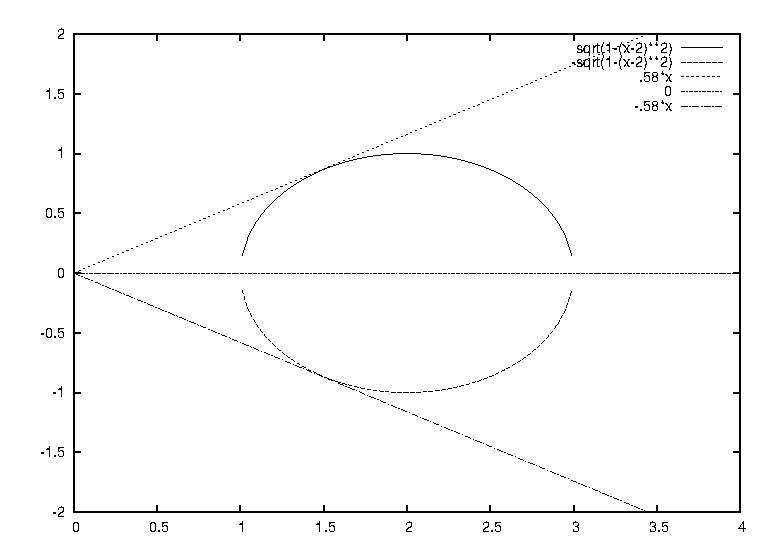
\includegraphics[width=450pt,height=450pt,angle=0]{shock.eps}
 \caption{衝撃波の伝播とMach角}
 \label{fig_shock}
 \end{center}
\end{figure}

\subsection{定常流の中の衝撃波}
最初に、定常的な流れの中の衝撃波について考える。圧縮性流体ではBernoulli
の定理が、
\begin{equation}
 h_0 = h + \frac{u^2}{2},
\end{equation}
で表される。

また、エントロピーは、エントロピーの保存則により、
\begin{equation}
 \bm{u}\cdot\text{grad}s = 0,
\end{equation}
である。そして、流れが一次源流の場合には$u ds/dl=0$なので、$s=Const.$で
ある。

圧縮性流体での質量流速は常に保存し、運動方程式とともに、
\begin{equation}
 j = \rho u,
\end{equation}
\begin{equation}
 \bm{u}\cdot\text{grad}\bm{u} = -\frac{1}{\rho}\text{grad}p,
\end{equation}
である。流線上では、運動方程式は、
\begin{equation}
 u\frac{du}{ds} = -\frac{1}{\rho}\frac{dp}{ds},
\end{equation}
となる。ここで、$s$はこの式でのみ弦長を表す。そして、これより、$udu =
-dp/\rho$が得られる。

ここで、音速の定義から$c^s = dp/d\rho$なので、$dp = c^2d\rho$で、
\begin{equation}
 d\rho u = 
  \rho\left(1-\frac{u^2}{c^2}\right),
\end{equation}
となる。この微分方程式から次のことがいえる。

\begin{enumerate}
 \item $1<u/c$の超音速のときは$d\rho u/du<0$であり、流速が大きくなると質
       量流束は小さくなり、流線が衝撃波から広がっていく
 \item $u/c<0$の亜音速のときは$0<d\rho u/du$であり、流速が大きくなると質
       量流束が大きくなり、流線が衝撃波へ集まっていく
 \item $u/c=1$のときには$d\rho u/du=0$で極大値を持つ
\end{enumerate}

このように流れの様子が亜音速から超音速へ遷移するときに大きく変わる。この
ように質量流束$j$が最大値$j_*$になる点での流速を臨界流速$u_*$と定義する。
そして、このとき$u=c$なので、$u_*=c$である。更にいえば、音速は圧力、密度
により変化する値なので、流速が変化にも影響を受ける。従って、臨界流速に対
応して、臨界音速$c_*$を定義できる。そして、このときにBernoulliの定理は、
\begin{equation}
 h_0 = h_* + \frac{c_*^2}{2},
\end{equation}
で表される。また、エントロピーも、
\begin{equation}
 s=s_*,
\end{equation}
である。そして、臨界音速は、
\begin{equation}
 c_* = c_0\sqrt{\frac{2}{\gamma - 1}},
\end{equation}
となる。

そして、熱力学の公式と、これら臨界流速のときの種々の熱力学関数の性質から、
臨界流速に達した際の圧縮性流体の性質を導くことができる。最初に、密度と、
圧力について、断熱圧縮の性質からもとめる。これは純粋に気体にだけ適用でき
る公式である。
\begin{equation}
 \rho = \rho_0
  \left(\frac{T}{T_0}\right)^{\frac{1}{\gamma - 1}},
\end{equation}
\begin{equation}
 p = p_0 \left(\frac{\rho}{\rho_0}\right)^{\gamma},
\end{equation}
が得られて、$c_PT=c^2/(\gamma - 1)$なので、これから、
\begin{equation}
 T_0 = T\left(1-\frac{\gamma - 1}{2}\frac{u^2}{c_0^2}\right)
  = T\left(1-\frac{\gamma - 1}{\gamma + 1}\frac{u^2}{c_*^2}\right),
\end{equation}
\begin{equation}
 \rho = 
  \rho_0 \left(
   1 - \frac{\gamma - 1}{2}\frac{u^2}{c_0^2}
  \right)^{\frac{1}{\gamma - 1}}
  = \rho_0 \left(
   1 - \frac{\gamma - 1}{\gamma + 1}\frac{u^2}{c_*^2}
	   \right)^{\frac{1}{\gamma - 1}},
\end{equation}
\begin{equation}
 p = p_0\left(
   1 - \frac{\gamma - 1}{2}\frac{u^2}{c_0^2}
\right)^{\frac{\gamma}{\gamma - 1}}
 = p_0\left(
   1 - \frac{\gamma - 1}{\gamma + 1}\frac{u^2}{c_*^2}
\right)^{\frac{\gamma}{\gamma - 1}}
\end{equation}
\begin{equation}
 u^2 = \frac{2c_0^2}{\gamma - 1}
  \left\{1-\left(\frac{p}{p_0}\right)^{\frac{\gamma - 1}{\gamma}}\right\}
  = \frac{2\gamma}{\gamma - 1}\frac{p_0}{\rho_0}
  \left\{1-\left(\frac{p}{p_0}\right)^{\frac{\gamma - 1}{\gamma}}\right\},
\end{equation}

\subsection{衝撃波断熱曲線}
衝撃波の一般的な性質、$p-V$曲線上での振る舞いについて考える。

最初に定常流について考える。一次元の定常流では、流速が空間的な保存量にな
る。それは衝撃波があるところ、ないところの区別なく成立するものなので、衝
撃波を挟んだ領域でも成立する。衝撃波の前縁を領域1、後縁を領域2とする。領
域1と領域2の間で各種流束は同じ値をとる。従って、
\begin{equation}
 \left[\rho u\right]^2_1 = 0, 
\end{equation}
\begin{equation}
 \left[\rho u^2 + p\right]^2_1 = 0,
\end{equation}
\begin{equation}
 \left[\rho u \left(h + \frac{u^2}{2}\right)\right]^2_1 = 0,
\end{equation}
となる。

ここで、質量流束を$j = \rho_2u_2 = \rho_1u_1$として定義すると、
\begin{equation}
 \rho_1u_1 = \rho_2u_2 = j,
\end{equation}
である。

次に、体積を比体積として、$V_1 = 1/\rho_1$、$V_2 = 1/\rho_2$と定義する。
このとき、質量流束と運動量流束の保存則から、
\begin{equation}
 u_1 = j V_1,\mspace{20mu}
  u_2 = j V_2,
\end{equation}
\begin{equation}
 p_1 + \rho_1 j^2 V_1^2 = p_2 + j^2V_2^2,
\end{equation}
が得られて、質量流束は、
\begin{equation}
 j^2 = \frac{p_1 - p_2}{V_2 - V_1},
\end{equation}
で表される。$0 < j^2$なので、$0 < p_1 - p_2$のときは$V_2 - V_1 < 0$で、
$p_1 - p_2 < 0$のときは$0 < V_2 - V_1$の関係にある。
また、流速差は、
\begin{equation}
 u_1 - u_2 
  = j \left(V_1 - V_2\right)
  = \sqrt{(P_2 - P_1) (V_1 - V_2)},
\end{equation}
で表される。

つぎに、これらの関係式をBernoulliの定理に代入する。
\begin{equation}
 h_1 - h_2 
  = \frac{1}{2}j^2 (V_2 - V_1)
  = \frac{1}{2}(p_1 - p_2) (V_1 + V_2),
\end{equation}
が得られる。これをRankine-Hunoiotの断熱曲線、または、衝撃波断熱曲線とい
う。

エンタルピーからエネルギーの形に形式をかえると、
\begin{equation}
 \epsilon_1 - \epsilon_2
  = \frac{1}{2}(p_1 + p_2) (V_2 - V_1),
\end{equation}
が得られる。

そして、このRankine-Hugoniotの断熱曲線は初期条件$p_1$、$V_1$により通る曲
線が代わる。領域1から1つめの衝撃波を超えて領域2にいき、そこから衝撃波2を
通って領域3へいく場合の変化は、$p_1\rightarrow p_2\rightarrow p_3$だが、
このときの$p_3$と、領域1から1つめの衝撃波を超え、衝撃波2を経ないで$p_3$
に至ったケースではそのときの熱力学的な状態量が変わってくる不可逆的な変化
になる。一方で、通常の断熱力線は、断熱曲線状で常に同じ経路で変化する。こ
れは衝撃波が散逸系の現象であることによるものである。

また、エントロピーは、エントロピー流束は保存しないので、保存量にはならな
い。これは衝撃波をまたぐとエントロピーが増加することを意味しており、粘性
のような散逸項のない現象の中で、ただ一つエントロピーが増加する現象である。

\subsection{弱い衝撃波}
Rankine-Hugoniotの断熱曲線の式を微小な変化量$s_1-s_2$、$p_2-p_1$の冪級数
展開で表す。この場合、$s_1-s_2$と$p_2-p_1$はそれぞれ級数展開が収束する程
度の微小な範囲で展開することになるので、ここで取り扱う現象も弱い衝撃波で
ある。
\begin{equation}
 h_2 - h_1
  = \frac{1}{2} (p_1 - p_2) (V_1 + V_2),
\end{equation}
について展開するが、エントロピーの微小変化と圧力の微小変化を求めるため、
エントロピーについては1次まで、圧力については3次の微少量まで展開する。
\begin{equation}
 h_2 - h_1 
  = \left.\frac{\partial h}{\partial s}\right|_p (s_2 - s_1)
  + \left.\frac{\partial h}{\partial p}\right|_s (p_2 - p_1)
  + \frac{1}{2}\left.\frac{\partial^2 h}{\partial p^2}\right|_s (p_2 - p_1)^2
  + \frac{1}{6}\left.\frac{\partial^3 h}{\partial p^3}\right|_s (p_2 - p_1)^3,
\end{equation}
だが、熱力学の公式から、$dh = Tds + VdP$なので、$h_s|_p=T$、
$h_p|_s=V$である。これを代入すると、
\begin{equation}
 h_2 - h_1 
  = T_1 (s_2 - s_1)
  + V_1 (p_2 - p_1)
  + \frac{1}{2}\left.\frac{\partial^2 h}{\partial p^2}\right|_s (p_2 - p_1)^2
  + \frac{1}{6}\left.\frac{\partial^3 h}{\partial p^3}\right|_s (p_2 - p_1)^3,
\end{equation}
が得られる。

また、Rankine-Hugoniotの断熱曲線の関係式から、体積について展開する。体積
はRankine-Hugoniotの関係式では圧力についての項しか含まれていない。
\begin{equation}
 V_2 - V_1 
  = \left.\frac{\partial V}{\partial p}\right|_s (p_2 - p_1)
  + \frac{1}{2} \left.\frac{\partial^2 V}{\partial p^2}\right|_s (p_2 - p_1)^2,
\end{equation}
が得られる。また、$dh=Vdp$から、$h_{pp} = V_p$が得られ、これらをまとめると、
\begin{equation}
 s_2 - s_1 = 
  \frac{V_{pp}|_s}{12T_1} (p_2 - p_1)^3,
\end{equation}
が得られる。この関係式から、衝撃波をまたいでのエントロピーの不連続は圧力
の不連続に比べて3次の微少量である。


\section{圧縮性流体の1次元流}
\section{一般的な性質}
圧縮性流体のときの、1次元流の運動方程式の空間積分。つまり、エネルギー保
存則は、上流側を$\emptyset_0$、考えている領域を$\emptyset$とすると、
\begin{equation}
 h_0 = h + \frac{u^2}{2},
\end{equation}
であり、これにエンタルピーと圧力、密度の関係を代入すると、
\begin{equation}
 u^2 = \frac{\gamma}{\gamma - 1}\left(
				 \frac{p_0}{\rho_0} - \frac{p}{\rho}\right),
\end{equation}
で、これに断熱圧縮の関係式を適用して、圧縮比により流速を評価しようとする
と、
\begin{equation}
 u^2 = \frac{2\gamma}{\gamma - 1}\frac{p_0}{\rho_0}
  \left\{1 - \left(\frac{p}{p_0}\right)^{\frac{\gamma - 1}{\gamma}}\right\},
\end{equation}
になり、$p=p^*$の地点で極大値を持つ。ここで、臨界圧力比を、
\begin{equation}
 p^* = p_0 \left(\frac{2}{\gamma - 1}\right)^{\frac{\gamma}{\gamma - 1}},
\end{equation}
で表せて、そのとき、$u=c^*$で、$\max (u) = c_0 \sqrt{2/(\gamma - 1)}$で
表される。

質量流束の保存則で考える場合、$d\rho u = \rho du + ud\rho$で、さらに、
$c^2=\gamma p/\rho$の関係式から、
\begin{equation}
 d\rho u = \rho \left(1 - \frac{u^2}{c^2}\right)du,
\end{equation}
であり、$u/c$について極大値を持つことが分る。ここで、やはり、$u=c$で臨界
値を持つ。

\section{ノズル流れ}
質量流量の定義を考える。
\begin{equation}
 Q = S \rho u,
\end{equation}
ここで、臨界流速以上に達した場合を考える。質量流束を$j$とすると、
\begin{equation}
 j = \left(\frac{p}{p_0}\right)^{\frac{1}{\gamma}}
  \sqrt{\frac{2\gamma}{\gamma - 1}\rho_0 p_0
 \left\{1-\left(\frac{p}{p_0}\right)^{\frac{\gamma-1}{\gamma}}\right\}},
\end{equation}
が得られる。この式をプロットすると図\ref{fig_flux_vs_pressure}のような関
係が得られる。横軸を膨張比、縦軸を質量流束としている。
前節で質量流束と速度の関係を求めたが、$u=c$になる場合に質量流束は極大値
を持った。従って、圧力が臨界圧力に達するときに質量流束も最大値をとる。

\begin{figure}[htbp]
 \begin{center}
  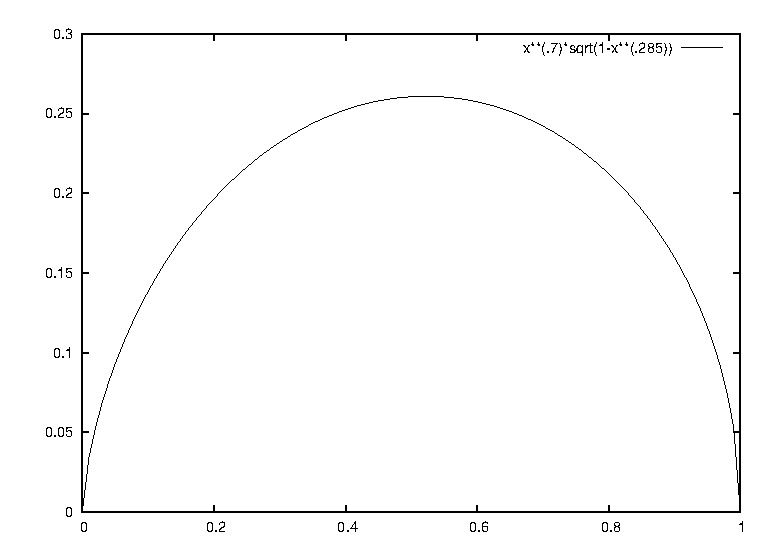
\includegraphics[width=450pt]{flux_vs_pressure.eps}
  \caption{質量流束と圧力比 (膨張比) の関係}
  \label{fig_flux_vs_pressure}
 \end{center}
\end{figure}


\section{音波}
\subsection{固有振動}
あつ閉じた境界の内部問題を考える場合は、考えている現象の方程式の境界値を
考える必要がある。それに対して、波動方程式の一般解は、開いた空間で与えら
れる。

また、有限の領域内での運動方程式はどのような振動数に対しても解を持つ訳で
はなく、固有振動数に対して解を持つ。固有振動数は容器の形に依存する。これ
を求めるために、境界条件のもとで運動方程式をとくことになる。

固有振動のオーダーは次元解析からすぐにわかり、波長$\lambda$、固有振動数
$\omega$はそれぞれ次のように与えられる。
\begin{equation}
 \lambda \sim l, \mspace{20mu}\gamma \sim \frac{l}{c},
\end{equation}
ここで、$l$は考えている領域の代表長さである。

次時、実際に速度ポテンシャルを$\phi = \phi_0(x,y,z)e^{-i\omega t}$と仮定
してみると、$\phi_0$について、
\begin{equation}
 \triangle \phi_0 + \left(\frac{\omega}{c}\right)^2\phi_0 = 0,
\end{equation}
のようなHelmholtzの方程式を得る。この方程式は一般的な、無限領域での条件
が与えられる場合は、$e^{ikr}$に比例するような解を持ち、$\phi_0=Const.$に
なるような、
\begin{equation}
 \phi = \phi_0 e^{i(\bm{k}\cdot\bm{r}-\omega t)},
\end{equation}
という一般解を持つ。

境界条件が決められている場合には、境界条件は実数で与えられているので、境
界値が実数を持つような解を選ばなければならない。また、領域内部では実数で
解が与えられるので、解$\phi_0$の共役複素数$\phi_0^*$もまた方程式の解であ
り、更に、共役複素数の公式から、$\phi_0\phi_0^*=|\phi_0|^2$なので、
\begin{equation}
 \phi_0 = f(x,y,z)e^{i\alpha},
\end{equation}
という方程式の形を取る。そして、速度ポテンシャルは、
\begin{equation}
 \phi = f(x,y,z)\cos (\omega t + \alpha),
\end{equation}
である。

このような波に対しては、特性曲線を定義することができず、明らかに伝播しな
い。このような波を定在波、定常波と呼ぶ。そして、固有振動は定在波である。

平面波を考える場合、
\begin{equation}
 \phi = a \cos\omega t cos \left(\frac{\omega x}{c}\right),
\end{equation}
となる。このとき、波数は$k=\omega /c$で、$x = n\pi c/ \omega$の点では常
に速度ポテンシャルは0になるような節を持つ。一方で、それらの中間になる点
は腹と呼ばれる。

\paragraph{直方体内部の固有振動数}
直方体の内部の速度ポテンシャルを、
\begin{equation}
 \phi = a \cos qx \cos ry \cos sz,
\end{equation}
とすると、$q^2 + r^2 + s^2 = \omega^2 / c^2$である。また、$q = m\pi /a$
のように任意の整数を定義すると、
\begin{equation}
 \omega^2 = c^2\pi^2
  \left(\frac{m^2}{a^2} + 
  \frac{n^2}{b^2} +
 \frac{p^2}{c^2}\right),
\end{equation}
が得られる。

\paragraph{Helmholtz共鳴管}
Helmholtz共鳴管の固有振動は、管の長さ$l$、断面積$S$とすると、管内の気体
の質量は$\rho S l$、管内の気体に作用する力は、$S (p_0-p)$である。これよ
り、運動方程式が、
\begin{equation}
 S\rho l u_t = S (p - p_0),
\end{equation}
として与えられる。一方で、音速の公式から、圧力変動と密度変動の関係は、
\begin{equation}
 \frac{\partial p}{\partial t} = 
  \frac{dp}{d\rho}
  \frac{\partial \rho}{\partial t},
\end{equation}
なので、これをまとめて、
\begin{equation}
 \frac{\partial^2p}{\partial t^2} = 
  -c^2\frac{\rho S u_t}{V} = 
  -c^2 \frac{S (p - p_0)}{lV},
\end{equation}
が得られる。

これより、この系の固有値が、
\begin{equation}
 \omega = c\sqrt{\frac{S}{lV}}、
\end{equation}
として得られ、これが固有振動数である。

\subsection{管内の音波}
管内を伝搬する音波の支配方程式を考える。このとき、管内の断面積は場所によっ
て変化すると仮定する。積分形式で書くと、質量保存則は、
\begin{equation}
 \int_{\Omega}dV\frac{\partial\rho}{\partial t}
  + \int_{\partial\Omega}dS\rho u = 0,
\end{equation}
であり、これを微分形式で書くと、
\begin{equation}
 S\frac{\partial\rho}{\partial t} +
  \frac{\partial\rho Su}{\partial x} = 0,
\end{equation}
が得られる。

音響近似した場合の運動方程式は、
\begin{equation}
 \frac{\partial u}{\partial t} 
  + \frac{1}{\rho}\frac{\partial p}{\partial x} = 0,
\end{equation}
で与えられる。

これらの方程式から、管内流の波動方程式を求める。

質量保存について、質量流束の項は、微小振幅波を仮定する場合には、
$u=O(\epsilon)$、$\rho_t = O(\epsilon)$のため、$(\rho u)_x = \rho u_x$と
いう近似ができる。これより、$S\rho_{tt} = \rho S u_{xt}$が得られる。これ
に運動方程式を代入すると、
\begin{equation}
 \frac{1}{S}\frac{\partial}{\partial x}
  \left(S\frac{\partial p}{\partial x}\right)
  -\frac{1}{c^2}\frac{\partial^2p}{\partial t^2} = 0,
\end{equation}
という波動方程式が得られる。

ここで、圧力について周期解を仮定すると、
\begin{equation}
  \frac{1}{S}\frac{\partial}{\partial x}
  \left(S\frac{\partial p}{\partial x}\right)
  -k^2p = 0,
\end{equation}
が得られる。

このような場合の簡単からの音の放射の強度は、
\begin{equation}
 I = \frac{\rho S^2\bar{u}_t^2}{4\pi c},
\end{equation}
で与えられる。

\subsection{音波の散逸}
音の散逸を考える。

音波の運動エネルギー$K$は、内部エネルギー$E_0$と熱の項$E(S)$から、
$K=E_0-E(S)$である。ここで、運動エネルギーの時間微分は、
$K_t =E_t(S)$である。そして、エネルギーのエントロピーによる微分は温度な
ので、$K_t = -T_0S_t$である。

熱伝導と粘性がある場合のエントロピーの保存則から、運動エネルギーの保存則
は次のように得られる。
\begin{equation}
 \frac{\partial K}{\partial t} = 
  \frac{-\kappa}{T}\int dV\left(\text{grad}T\right)^2 -
  \frac{1}{2}\mu\int dV
  \left(\frac{\partial u_k}{\partial x_i} +
   \frac{\partial u_i}{\partial x_k} -
   \frac{2}{3}\delta_{ik}\frac{\partial u_j}{\partial x_j}
  \right)^2 - 
  \Theta\int dV\left(\text{div}\bm{u}\right)^2.
\end{equation}
そして、音波が$x$方向にだけ進行するとすると、
\begin{equation}
 \frac{\partial K}{\partial t} = 
  \frac{-\kappa}{T}\int dV \left(\frac{\partial T}{\partial x}\right)^2 -
  \frac{4}{3}\mu\int dV
  \left(\frac{\partial u}{\partial x}\right)^2 - 
  \Theta\int dV\left(\frac{\partial u}{\partial x}\right)^2,
\end{equation}
が得られる。

また、このときの固有関数を$u = u_0 \cos (kx - \omega t)$とする。これによ
り、粘性の項は、
\[
   \frac{4}{3}\mu\int dV
  \left(\frac{\partial u}{\partial x}\right)^2 - 
  \Theta\int dV\left(\frac{\partial u}{\partial x}\right)^2
  = -k^2\left(\frac{4}{3}\mu + \Theta\right) u_0^2
  \int dV\mspace{5mu}\sin^2 (kx - \omega t),
\]
平均値は、$-k^2(4/3\mu + \Theta)u_0^2V_0/2$になる。

熱伝導の項は、温度と流早の関係が与えられることから求めることができる。温
度と圧力の関係は$dT=(\partial_pT)|_sdp$なので、$T_p|_s=T/c_pV_T|_p$と、
$v=p/(\rho c)$から、次のように得られる。
\[
 T_t = c\beta T\frac{u}{c_p}.
\]
ここで、$\beta$は熱膨張係数で、$\beta =V_T|_p/V$で表される。この関係から、
\[
 \frac{\partial T}{\partial x} 
 = \frac{\beta c T}{c_p}\frac{\partial u}{\partial x}
 = -\frac{\beta c T}{c_p}u_0k\sin(kx - \omega t)m,
\]
が得られる。ここで、
\[
 c_p - c_v 
 = \beta^2 T \left.\frac{\partial p}{\partial\rho}\right|_T
 = \beta^2 T \left(\frac{c_v}{c_p}\right)
 \left.\left(\frac{\partial p}{\partial \rho}\right)\right|_S
 = \beta^2Tc^2\frac{c_v}{c_p},
\]
という関係式があるので、$-k(1/c_v-1/c_p)k^2u_0^2V_0/2$となる。

これらをまとめると、
\begin{equation}
 \frac{\partial K}{\partial t}
  = -\frac{1}{2}k^2u_0^2V_0
  \left[\left(\frac{4}{3}\mu + \Theta\right)
  + \gamma\left(\frac{1}{c_v}-\frac{1}{c_p}\right)\right],
\end{equation}
のように散逸の関係式が得られる。ここで、減水係数のような形式で表そうとす
ると、$e^{-\kappa x}$のように減衰するとすると、
\begin{equation}
 \kappa = \frac{\left| K \right|}{2cE},
\end{equation}
のようになり、
\begin{equation}
 \kappa = \frac{\omega^2}{2\rho c}
  \left[\left(\frac{4}{3}\mu + \Theta\right)
  + \gamma\left(\frac{1}{c_v}-\frac{1}{c_p}\right)\right],
\end{equation}



\chapter{流体の不安定性}
Reynolds数が大きい場合の流れの安定性を考える。臨界Reynolds数$Re_c$に対し
て、$Re<Re_c$の場合は、安定なので、その場合は$\omega=\omega_r+i\omega_i$
のうち$\omega_i$は負の値を取り、中立不安定の場合は$\omega_i=0$であり、
$Re_c<Re$の場合には$\omega_i$は正の値をとる。ただ、不安定性がそれ程多く
ない領域では$\omega_i<\omega_r$のように観測的に見れる。
ここで、流速の1次の微少量の項$\bm{u}_1$について、
\begin{equation}
 \bm{u}_1 = A(t)\bm{f}(x,y,z),
\end{equation}
と表せると仮定し、更に、
\begin{equation}
 A(t) = \alpha e^{-i(\omega_r + i\omega_i)t},
\end{equation}
で表される。
ここで、$A(t)$は流れに乱れが発生し始めてすぐの時間でだけ成り立つ。
$e^{\omega_it}$は急速に増加するため、このような近似は乱れが発生してから
の短い時間でしか適用できない。$Re\simeq Re_c$で、$Re_c<Re$のような状況を
考える。
流れの乱れのパラメータとして、$|A(t)|^2$を考えて、その時間発展を考える。
\begin{equation}
 \frac{d|A|^2}{dt} = 2\omega_i |A|^2,
\end{equation}
のように、$\omega_i$が$|A|^2$の固有値として現れる。更に、高次の項まで考
えると、
\begin{equation}
  \overline{\frac{d|A|^2}{dt}} = 2\omega_i |A|^2 - \beta |A|^4,
\end{equation}
で、これを解くと、
\begin{equation}
 \frac{1}{|A|^2} = \frac{\beta}{2\omega_i} + \beta e^{-2\omega_it} ,
\end{equation}
で、$|A|^2$の漸近解が得られる。
\begin{equation}
 |A|^2\rightarrow\frac{2\omega_i}{\beta},
\end{equation}
更に、乱れの広がりがReynolds数に比例すると考えると、$\omega_i\sim
Re-Re_c$と仮定できるので、
\begin{equation}
 |A|\rightarrow \sqrt{Re-Re_c},
\end{equation}
となり、乱流の乱れはReynolds数の平方根にある程度までは比例する。更にそれ
よりも乱れが大きくなる場合は2次の微少量についても考慮することになる。

\section{境界層}
\subsection{境界層方程式}

壁面流れについて、特異摂動法による解法の1つとして、壁面近傍の境界層内部を近方場、境
界層の外側の主流を遠方場として考える。境界層外縁での境界条件を決めて解の
接合を行う。
特徴を箇条書きで書くと。
\begin{enumerate}
 \item 定常流を仮定する
 \item 境界層厚さ$\delta$は十分に薄いと仮定して、$v\ll u$
 \item 流速は$y$方向に$\delta$のオーダーの空間で急激に変化する
 \item 流速は$x$方向に$l$のオーダーで緩やかに変化する
\end{enumerate}
上記の考察から、$\partial\emptyset/\partial x = O(\emptyset/l)$であ
り、$\partial\emptyset/\partial y = O (\emptyset/\delta)$である。この仮
定から、運動方程式の各項は、
\begin{equation}
 \frac{\partial\emptyset}{\partial x} \ll
  \frac{\partial\emptyset}{\partial y}, \mspace{30mu}
 \frac{\partial^2\emptyset}{\partial x^2} \ll
  \frac{\partial^2\emptyset}{\partial y^2}, 
\end{equation}
の近似から、
\begin{equation}
 u\frac{\partial u}{\partial x}
\end{equation}
また、$x$方向と$y$方向の圧力勾配は、それぞれの方向の流速に比例するオーダー
と仮定すると、運動方程式の$x$方向と$y$方向成分から、その比率
$(\partial p/\partial y)/(\partial p/\partial x) = v / u$なので、これよ
り$y$方向の方程式は$\partial p/\partial y \simeq 0$と近似できる。

以上より、境界層内部での運動方程式と連続の式は、
\begin{equation}
 u\frac{\partial u}{\partial x}
 + v\frac{\partial u}{\partial y}
 = -\frac{1}{\rho}\frac{\partial p}{\partial x}
 + \nu \frac{\partial^2u}{\partial y^2},
\end{equation}
\begin{equation}
 \frac{\partial p}{\partial y} = 0,
\end{equation}
\begin{equation}
 \frac{\partial u}{\partial x}
  + \frac{\partial v}{\partial y}
  = 0,
\end{equation}
である。一方で、境界層外部はポテンシャル流れであるとすると、単純に
Bernoilliの定理が成り立っていると考えると、
\begin{equation}
 \frac{1}{2}\rho U^2 + P = Const.,
\end{equation}
である。

ここで、境界層外縁での方程式系の接合を考える。

境界層内部の運動方程式より、$p=p(x)$であり、これより境界層内部では$y$方
向に圧力分布がない上に、圧力は$x$方向について与えられた関数になる。これ
が境界層の内部で常に成り立っているため、当然境界層外縁でも成立する。従っ
て、境界層外縁での主流の圧力もまた流れ方向$x$に対してのみ分布を持つこと
になる。これより、境界層外部でも圧力は$y$方向に分布を持たないことから、
圧力と流速の関係が得られる。また、境界層外部の圧力が即ち境界層内部の圧力
となる。

ここで、境界層外部で成立してるBernoulliの定理を$x$方向について微分すると、
\begin{equation}
 \frac{\partial P}{\partial x} = -\rho U \frac{\partial U}{\partial x},
\end{equation}
これを境界層内部の運動方程式に代入すると、所謂境界層方程式が以下のような
形式で得られる。
\begin{equation}
 u\frac{\partial u}{\partial x} 
 +v\frac{\partial u}{\partial y} 
 -\nu\frac{\partial^2u}{\partial y^2}
 = U\frac{\partial U}{\partial x},
\end{equation}
\begin{equation}
 \frac{\partial u}{\partial x}
  +\frac{\partial v}{\partial y}
  = 0.
\end{equation}

\subsection{Reynolds相似}
境界層方程式を次のような無次元化を施す。
\begin{align}
 x'=\frac{x}{l}, & y' = \frac{\sqrt{Re}}{l}y, \\
 u' = \frac{u}{U}, & v = \sqrt{Re}\frac{v}{U}.
\end{align}
ここで、微分は次のように変数変換される。
\begin{equation}
 \frac{\partial}{\partial x} = \frac{1}{l}\frac{\partial}{\partial x'},
  \mspace{25mu}
  \frac{\partial}{\partial y} = \frac{\sqrt{Re}}{l}\frac{\partial}{\partial y},
\end{equation}
これを境界方程式に適用すると、
\begin{equation}
 u\frac{\partial u}{\partial x}
  + v\frac{\partial u}{\partial y}
  - \frac{\partial^2U}{\partial y^2}
  = U\frac{\partial U}{\partial x},
\end{equation}
\begin{equation}
 \frac{\partial u}{\partial x} 
  +\frac{\partial v}{\partial y} = 0,
\end{equation}
が得られる。

これより境界層があるような流れでは、流れ場はReynolds数に依存しないため、
Reynolds数に対して相似性がある。特に、$v$と$y$はReynolds数によりスケール
される。
また、これより無次元化された境界層方程式は全て0次の微少量なため、
$v'=\sqrt{Re}/Uv=O(1)$、$y'=\sqrt{Re}/ly=O(1)\equiv \delta$のため、
\begin{equation}
 \delta = \frac{l}{\sqrt{Re}}, \mspace{25mu}
  v = \frac{U}{\sqrt{Re}},
\end{equation}
のような関係が得られ、境界層厚さ、流れと垂直方向の流れはReynolds数の変化
に影響を受けることが分る。

次に半無限の平板上を流れる流れを考える。ここで、$U=Const.$として、
$\partial U/\partial x=0$なので、
\begin{equation}
 u\frac{\partial u}{\partial x}
  + v\frac{\partial u}{\partial y}
  - \nu\frac{\partial^2u}{\partial y^2} = 0,
\end{equation}
\begin{equation}
 \frac{\partial u}{\partial x} 
  +\frac{\partial v}{\partial y} = 0,
\end{equation}
だが、このような場合には特徴的な長さ$l$を定義できない。従って、無次元化
を$x$、$y$の組み合わせで行って、Reynolds相似になるようなものを変数に選ぶ。
無次元化にReynolds数が関わるのは$y$と$v$で、それぞれ以下のようである。
\[
 v' = \sqrt{\frac{l}{\nu U}}v, \mspace{25mu}
 y' = \sqrt{\frac{U}{\nu l}}y.
\]
これより、
\begin{equation}
 y\longrightarrow \frac{y'}{\sqrt{x'}} = \sqrt{\frac{U}{\nu x}} y,
\end{equation}
\begin{equation}
 v\longrightarrow \sqrt{x}v = \sqrt{\frac{x}{\nu x}}y,
\end{equation}
のような無次元化が仮定できる。これは$v$と$y$に$l$が入らない形式であり、
解を次のように仮定する。
\begin{equation}
 u = U f \left(\sqrt{\frac{U}{\nu x}y}\right), \mspace{25mu}
  v = \sqrt{\frac{U \nu}{x}} g \left(\sqrt{\frac{U}{\nu x}y}\right),
\end{equation}
これを連続の式に代入することで$f$と$g$の関係が得られる。
\begin{equation}
 \xi = \sqrt{\frac{U}{\nu x}}y,
\end{equation}
\begin{equation}
 f(\xi) = \phi_{\xi},
 % \frac{\partial\phi}{\partial\xi} = f(\xi),
\end{equation}
\begin{equation}
 g(\xi) = \frac{1}{2}\left(\xi \phi_{\phi} - \phi\right).
\end{equation}
 これを運動方程式に適用すると、
\begin{equation}
 \phi\phi_{\xi\xi} + 2\phi_{\xi\xi\xi} = 0,
\end{equation}
 が得られる。

 更に、$u$の変数変換は、$u = U f(\xi)$であることから、
 $0\leq f(\xi) \leq U$であり、$y = \delta$で$f(\xi) = 1$になることが特異
 摂動法の解の接合の考え方から見込まれる。従って、境界層厚さは、半無限の平
 板上では、
\begin{equation}
 \delta \simeq \sqrt{\frac{\nu x}{U}},
\end{equation}
 のようなオーダーとして与えられる。


\subsection{境界層の剥離}
無限遠までつづく平板を考えたときに、境界層は主流につられて徐々に発達して
いく。境界層内部では粘性が卓越し、有限の渦度を持ち、一方で、主流は乱れが
十分発達しているため、そのような場合は非粘性を仮定できるため、一般的に渦
度が0になる。そして、渦度が境界層内部で生成され、それが主流へ拡散してい
く。ただし、そのような状態は循環の保存則とは矛盾するためある種の特異点に
なる。また、そのような状態は平板に対する垂直方向の速度成分が発散するため、
そのような状態を仮定して、境界層方程式に適用することで検討を進める。

最初に、境界層の剥がれ点を$x_0$と仮定する。また、そこでの$v$は十分大きく、
$v(x_0,y)\rightarrow\infty$と仮定できる。更に、その微分も十分大きい数値
を取ると仮定できて、$\partial v/\partial y \rightarrow\infty$とする。
これを連続に式に適用すると、$\partial u/\partial x\rightarrow\infty$であ
る。これより、逆に$\partial x/\partial u=0$であり、剥がれ点の場所を流速
の関数として、流速で展開することができる。また、$v(x_0,y)=u_0(y)$として
剥がれ点での垂直方向の流速は$y$だけの関数である。

ここで、$x_0$を$u$で展開する。ただし、$\partial x/\partial u=0$なので、
\begin{equation}
  x_0-x = \frac{1}{2}\frac{\partial^2x}{\partial u^2} (u_0 - u)^2,
\end{equation}
である。これより、流速は逆に流れ方向の関数として与えられて。
\begin{equation}
 u = u_0(y) + \alpha (y)\sqrt{x_0-x},
\end{equation}
がえられる。一方で、連続の式から、
\[
 v = -\int dy \frac{\partial u}{\partial x},
\]
なので、
\begin{equation}
 v = \frac{\beta(y)}{2\sqrt{x_0-x}},
\end{equation}
である。

また、境界層方程式に立ち返ると、圧力項と粘性項はそれぞれ圧力勾配が有限の値を
取ること、流速の2階微分は有限の値を取ることがわかる。一方で、移流項は流
速の1階微分なので、無限大に発散する。ただし、方程式が成り立つには、これ
らが互いに相殺しなければならない。従って、$uu_x + vu_y=0$でなければなら
ない。これと連続の式$u_x+v_y=0$より、
\begin{equation}
 \frac{\partial}{\partial y}\frac{v}{u}=
  \frac{\partial}{\partial y}\frac{\beta(y)}{u_0(y)\sqrt{x_0-x}}
\end{equation}
これより、$v/u$は$x$だけの関数なので、$\beta=Au_0(y)/2$でなければならな
い。また、$\alpha=Adu_0/dy$なので、
\begin{equation}
 u = \frac{Au_0(y)}{2\sqrt{x_0-x}},
\end{equation}
\begin{equation}
 v = u_0(y)+A\left(\frac{du}{dy}\right)\sqrt{x_0-x},
\end{equation}
 である。

ここで、流れと垂直方向の方向の流速は$x_0$に近づくにつれて無限大に近づき、
更に、$x_0<x$では$u$、$v$ともに虚数解を持つため、境界層方程式は意味のあ
る解を持たなくなることがわかる。また、粘着条件から、
$u|_{x=x_0}=v|_{x=x_0}=0$であるから、
\begin{equation}
 u_0(0) = 0, \mspace{25mu} \left.\frac{du_0}{dy}\right|_{y=0} = 0,
\end{equation}
であることがわかる。これより、$A\neq 0$の場合には境界層の剥離が発生する
ことが分る。一方で、$A=0$のときには境界層の剥離は発生しない。その場合は、
$u$は流れ方向に進行するに連れて$u$は加速していくが、$x_0<x$に達した場合
に$\partial u/\partial x<0$となり、減速し、逆流が発生する。この場合は渦
度は境界層内部から主流へは拡散しては行かない。

\section{Orr-Sommerfeld方程式}
流体の不安定性を流れ関数を導入して検討する。非圧縮の2次元の運動方程式を
考えることで、流れ関数の導入が可能である。また、それにあたって運動方程式
から渦度方程式を経由して考える。

最初に、2次元での渦度と流れ関数について、
\begin{equation}
 \omega = \frac{\partial v}{\partial x} 
  - \frac{\partial u}{\partial y},
\end{equation}
\begin{equation}
 u = \frac{\partial \psi}{\partial y}, \mspace{25mu}
  v = -\frac{\partial \psi}{\partial x},
\end{equation}
のように定義する。これにより、渦度と流れ関数は、$\omega=-\triangle\psi$
で与えられる。

一方で、渦度方程式を導出する。3次元の場合の運動方程式にrotを取ることで渦
度方程式が求められるが、それは、
$\epsilon_{ijk}\partial / \partial x_j$を左から$\emptyset_i$に掛けること
で得られる。

今、粘性を考慮した場合の運動方程式は
\begin{equation}
 \frac{\partial u_i}{\partial t}
  + u_j\frac{\partial u_i}{\partial x_j}
  = -\frac{1}{\rho}\delta_{ij}\frac{\partial p}{\partial x_j}
  + \nu\frac{\partial}{\partial x_j}
  \left(\frac{\partial u_i}{\partial x_j} + \frac{\partial u_j}{\partial x_i}\right),
\end{equation}
であるが、これから、渦度方程式が、
\begin{equation}
 \frac{\partial\omega_i}{\partial t}
  + u_j\frac{\partial \omega_i}{\partial x_j}
  + \omega_j\frac{\partial u_i}{\partial x_j}
  = \nu\delta_{jk}\frac{\partial^2\omega_i}{\partial x_j\partial x_k},
\end{equation}
で得られる。これを2次元に適用する場合は、渦度による流れ場の伸長の項は消
える。また、$z$方向の渦度を$\omega$と考えることで、
\begin{equation}
 \frac{\partial\omega}{\partial t}
  + u\frac{\partial\omega}{\partial x}
  + v\frac{\partial\omega}{\partial y}
  = \nu\triangle\omega,
\end{equation}
である。

ここで、流れ方向の流速に摂動を取る。
\begin{equation}
 \psi(x,y,t) = \int_{0}^{y}dy U(y) + \tilde{\psi}(x,y,t),
\end{equation}
により、
\begin{equation}
 u = U + \frac{\partial\tilde{\psi}}{\partial y}, \mspace{25mu}
  v = -\frac{\partial\tilde{\psi}}{\partial x},
\end{equation}
が得られる。ただし、$U=O(1)$、$\tilde{¥psi}=O(\epsilon)$である。
これをもとの方程式に適用して、1次の微少量と2次の微少量にわけると、
\begin{align}
 \frac{\partial}{\partial t}\triangle\tilde{\psi}
  + U\frac{\partial}{\partial x}\triangle\tilde{\psi}
  = \frac{\partial\tilde{\psi}}{\partial x}\frac{\partial^2U}{\partial
  y^2} 
  + \nu\triangle^2\tilde{\psi}, & & O(\epsilon),  \label{proto_orr-sommerfeld}\\
  \frac{\partial\tilde{\psi}}{\partial y}
  \frac{\partial}{\partial x}\triangle\tilde{\psi}
  -  \frac{\partial\tilde{\psi}}{\partial x}
  \frac{\partial}{\partial y}\triangle\tilde{\psi} = 0, & & O(\epsilon^2) 
\end{align}
が得られる。

ここで、解を$\tilde{\psi}(x,y,t)=\phi(x)e^{i(kx-\omega t)}$と仮定して、
$y$方向の分布を考えると、
\begin{equation}
 (U-c)(\phi_{yy}-k^2\phi) = \phi U_{yy}
  + \frac{\nu}{ik}\left(k^2-\frac{\partial^2}{\partial y^2}\right)^2\phi,
\end{equation}
としてOrr-Sommerfeld方程式が得られる。ここで、$\omega = ck$として位相速
度$c$を仮定した。Orr-Sommerfeld方程式の問題では$\phi$を$y$の4階の微分方程
式として求めることで、解を$x$、$t$について級数和をとりもとの厳密解を得る
ことが出来る。この方程式は既知の$U$を使って$\phi$についての線形方程式を
解く問題になり、外部から与えられる主流$U$について$\phi$の固有値を解く問
題になる。これをOrr-Sommerfeld固有値の問題という。

今、方程式系を(\ref{proto_orr-sommerfeld})まで戻って考えたとき、
主流は$y$方向について均一とすると、$U_{yy}=0$となり、1次の項は
$\triangle\tilde{\psi}$についての移流拡
散方程式のような形式をとる。
\begin{equation}
  \frac{\partial}{\partial t}\triangle\tilde{\psi}
  + U\frac{\partial}{\partial x}\triangle\tilde{\psi}
  = \nu\triangle^2\tilde{\psi},
\end{equation}
ここで$\triangle\psi$は誤差関数を解として、更にそこから$\psi$を誤差関数
をGreen関数として計算することで少なくとも形式解を得ることが出来る。

\subsection{渦度方程式からの解法}
ここで、移流拡散方程式を解くために、$\tau = t - x/U$と仮定すると、
$\partial/\partial\tau=\partial/\partial t +U\partial/\partial x$となる。
また、境界層方程式の導出からの洞察を援用して、$\tilde{v}\simeq\tilde{u}$、
$\tilde{u}_x\ll\tilde{v}_x$、となるため、
$\triangle\tilde{\psi}\simeq\tilde{\psi}_{xx}$と仮定する。このため、
$\Psi\equiv\tilde{\psi}_xx$と置くと、
\begin{equation}
 \frac{\partial\Psi}{\partial \tau}=\nu\frac{\partial^2\Psi}{\partial x^2},
\end{equation}
となる。ここで、この移流拡散方程式を教科書的な解法に則って解いていく。変
数分離法を使うことで、この方程式の固有値を$\lambda$と仮定すると、
\begin{equation}
 \Psi = \int_{-\infty}^{\infty}\mspace{5mu}
  e^{\lambda}\left\{a(\lambda)e^{\sqrt{\frac{\lambda}{\nu}}x}+
	     b(\lambda)e^{-\sqrt{\frac{\lambda}{\nu}}x}\right\},
\end{equation}
が得られる。ここで問題にしているのは1次の微少量についてであり、更に初期
値問題を扱っているため、初期条件は全ての空間で解が穏やかであることである。
また、空間的な境界条件についてはノズル出口では0が仮定できるが無限遠、ま
たは有限区間でのある程度の擾乱について認める必要がある。仮に不安定性の議
論をする場合に、境界条件に無限大に発散する条件を認めることは数学的に不適
切である。
そこで、有限区間で有限振幅の乱れに達すると仮定する。例えば、$x=L$のとき
に$\tilde{v}=V$と仮定しておくことで後で漸近解を得ることができるかもしれ
ない。

初期条件の適用にあたっては、$\Psi|_{t=0}=0$とすると、$a(\lambda)$、
$b(\lambda)$について自明解しか選べないように見受けられる。これが非自明解
を持つ条件は、


\section{2次元直交座標系のKelvin-Helmholtz不安定}
2相流の解析を行うにあたって、相の間の界面は流体の方程式がもつ非線形性に
よりReynolds数が大きくなるに従い無限の自由度を持ってくるため非常に複雑な
形になってくる。そこで、摂動法や、線形安定解析により不安定性を評価する。
\subsection{非粘性比圧縮の場合の線形安定解析}
流速$\bm{u}$を定常流を仮定できる主流$\bm{u}_0$と非定常な乱れの成分
$\bm{u}_1$にわけて、$\bm{u}(t,x,y)=\bm{u}(x,y)+\bm{u}_1(t,x,y)$とする。
ここで、$\bm{u}_0=O(1)$、$\bm{u}_1=O(\epsilon)$とする。
まず最初に、非粘性の場合を考えるが、これを非粘性の流体の運動方程式に適用する
と、
\begin{equation}
\begin{cases}
 \bm{u}_0\cdot\text{grad}\bm{u}_0 = -\frac{1}{\rho}\text{grad}p_0, 
 &O(1), \\
 \frac{\partial\bm{u}_1}{\partial t} + \bm{u}_0\cdot\text{grad}\bm{u}_1
 = -\frac{1}{\rho}\text{grad}p_1,
 & O(\epsilon), \\
 \bm{u}_1\cdot\text{grad}\bm{u}_1 = 0,
 & O(\epsilon^2), \\
\end{cases}
\end{equation}
のように支配方程式が与えられる。

今、主流はポテンシャル流で与えられているとして、1次の微少量のみ解く。ここで、完全流体を仮定した場合に
$O(\epsilon)$の項は以下のように与えられる。
\begin{equation}
 \frac{\partial u_1}{\partial t}
  +u_0\frac{\partial u_1}{\partial x}
  = -\frac{1}{\rho}\frac{\partial p}{\partial x},
\end{equation}
\begin{equation}
 \frac{\partial v_1}{\partial t}
  +u_0\frac{\partial v_1}{\partial x}
  = -\frac{1}{\rho}\frac{\partial p}{\partial y},
\end{equation}
\begin{equation}
 \frac{\partial u_1}{\partial x}
  + \frac{\partial v_1}{\partial y} = 0,
\end{equation}
また、ここで、運動方程式の両辺にdivを掛けると、圧力については$\triangle p_1=0$
が成立する。

まず、流速の流れ方向成分は流れ方向に変化しないと仮定する。
その上で、流速、圧力ともに次のように解を仮定する。
$u_1=\tilde{u}_1e^{i(kx-\omega t)}$、
$v_1=\tilde{v}_1e^{i(kx-\omega t)}$、
$p_1=\tilde{p}_1f(y)e^{i(kx-\omega t)}$。これを方程式に代
入すると、
$p=\tilde{p}_1(e^{ky}+e^{-ky})$
がえられるが、流れと鉛直方向に解が収束しなければならないので、
\begin{equation}
 p=\tilde{p}_1e^{-ky},
\end{equation}
となる。また、流速については、
\begin{equation}
 (-i\omega + iku_0)\tilde{u}_1
  = \frac{1}{\rho}ik\tilde{p}_1,
\end{equation}
\begin{equation}
 (-i\omega + iku_0)\tilde{v}_1
  = \frac{1}{\rho}ik\tilde{p}_1,
\end{equation}
となり、
\begin{equation}
 v_1=\tilde{v}_1\frac{k\tilde{p}_1}{i\rho (ku_0-\omega)},
\end{equation}
が得られる。

ここで、界面$\zeta=\zeta(t,x)$についての境界条件を考える。

運動学の条件は、
\begin{equation}
 \frac{\partial\zeta}{\partial t}+u_0\frac{\partial\zeta}{\partial x} 
  = v_1,
\end{equation}
力学的条件は界面での応力の連続性から得られて、気体側の圧力を$p_a$とする
と、
\begin{equation}
 \frac{1}{2}\rho \bm{u}^2 + p = p_a,
\end{equation}
である。

ここで、界面の位置も固有問題で与えられると仮定して、方程式の解を代入すると、
\begin{equation}
 \omega =
  ku_0\frac{\rho\pm i\sqrt{\rho\rho_a}}{\rho+\rho_a},
\end{equation}
のような分散関係式が得られる。この関係から、$0<\Re[\omega]$が常に成り立
つため、このような流れは常に不安定である。

\subsection{非圧縮の粘性流体の安定解析の支配方程式}
粘性非圧縮の場合を考える。
\begin{equation}
 \frac{\partial u}{\partial t} 
  + u\frac{\partial u}{\partial x}
  + v\frac{\partial u}{\partial y}
  = -\frac{1}{\rho}\frac{\partial p}{\partial x}
  + \frac{1}{Re}\triangle u,
\end{equation}
\begin{equation}
 \frac{\partial v}{\partial t} 
  + u\frac{\partial v}{\partial x}
  + v\frac{\partial v}{\partial y}
  = -\frac{1}{\rho}\frac{\partial p}{\partial y}
  + \frac{1}{Re}\triangle v,
\end{equation}
\begin{equation}
 \frac{\partial u}{\partial x}
  + \frac{\partial v}{\partial y}
  = 0.
\end{equation}
摂動を考える。
\begin{equation}
 u=\left\{\left.U\right|U=Const.=O(1)\right\},
\end{equation}
\begin{equation}
 v=\left\{\left.\tilde{v}\right|\tilde{v}=\tilde{u}(x,t)=O(\epsilon)\right\},
\end{equation}
これをもとに運動方程式を整理して、1次の微少量の項を抜き出すと、
\begin{equation}
 \frac{\partial p}{\partial x} = 0,
\end{equation}
\begin{equation}
 \frac{\partial v}{\partial t} 
  + U\frac{\partial v}{\partial x}
  = -\frac{1}{\rho}\frac{\partial p}{\partial y}
  + \frac{1}{Re}\frac{\partial^2v}{\partial x^2},
\end{equation}
\begin{equation}
 \frac{\partial v}{\partial y} = 0,
\end{equation}
で、更に、運動方程式にdivを掛けることで圧力についてLaplace方程式が得られ
る。また、簡単のため$\tilde{\emptyset}$は$\emptyset$とした。
\begin{equation}
 \frac{\partial^2p}{\partial y^2}=0,
\end{equation}
これらから微少量については解を求められる。
\begin{equation}
 v=v(x,t)=\bar{v}e^{i(kx-\omega t)},
\end{equation}
\begin{equation}
 p=\left\{\left.\bar{p}_yy+\bar{p}_0\right|\bar{p}_y=\bar{p}_y(t),\bar{p}_0=\bar{p}_0(t)\right\},
\end{equation}
これを運動方程式のy方向の方程式に代入することで、圧力と流速の関係を得る。
\begin{equation}
 \left(\omega+kU-\frac{k^2}{Re}\right)\bar{v} = \frac{\bar{p}_y}{\rho}
\end{equation}
\subsection{自由表面の場合}
境界条件は、運動学の条件と、力学的な条件を考えるが、力学的な条件として、
界面での圧力の連続性を考える。また、界面の位置を$Y$とする。
\begin{equation}
 \frac{\partial Y}{\partial t}+U\frac{\partial Y}{\partial x}=v,
\end{equation}
\begin{equation}
 p=p_{\infty}
\end{equation}
また、界面について、$Y=\eta e^{i(kx - \omega t)}$と仮定すると、運動学の
条件から、
\begin{equation}
 i(kU-\omega)\bar{v}=\eta,
\end{equation}
が得られ、更に、力学的条件から、
\begin{equation}
 \bar{p}_yY+\bar{p}_0 = p_{\infty},
\end{equation}
が得られる。
\section{円筒座標系のKelvin-Helmholtz不安定}
\subsection{支配方程式}
円筒座標系の非圧縮粘性の運動方程式と連続の式。
\begin{equation}
 \frac{\partial u_r}{\partial t} + u_r\frac{\partial u_r}{\partial r}
  + \frac{u_\theta}{r}\frac{\partial u_r}{\partial\theta} +
  u_z\frac{\partial u_r}{\partial z} = 
  -\frac{1}{\rho}\frac{\partial p}{\partial r} 
  + \nu \left(\frac{\partial^2u_r}{\partial r^2}
	+\frac{1}{r}\frac{\partial u_r}{\partial r}
	+\frac{1}{r^2}\frac{\partial^2u_r}{\partial\theta^2}
	-\frac{2}{r^2}\frac{\partial^2u_{\theta}}{\partial\theta}
	-\frac{u_r}{r^2}
	+\frac{\partial^2u_r}{\partial z^2}\right),
\end{equation}
\begin{equation}
 \frac{\partial u_{\theta}}{\partial t} + \cdots,
\end{equation}
\begin{equation}
 \frac{\partial u_z}{\partial t} + u_r\frac{\partial u_z}{\partial r}
  + \frac{u_\theta}{r}\frac{\partial u_z}{\partial\theta} +
  u_z\frac{\partial u_r}{\partial z} = 
  -\frac{1}{\rho}\frac{\partial p}{\partial z} 
  + \nu \left(\frac{\partial^2u_z}{\partial r^2}
	 +\frac{1}{r}\frac{\partial u_z}{\partial r}
	+\frac{1}{r^2}\frac{\partial^2u_z}{\partial\theta^2}
	+\frac{\partial^2u_z}{\partial z^2}
	\right),
\end{equation}
\begin{equation}
 \frac{\partial u_r}{\partial r} + \frac{u_r}{r}
  +\frac{1}{r}\frac{\partial u_\theta}{\partial \theta}
	+\frac{\partial u_z}{\partial z} = 0.
\end{equation}
軸対称、周方向流速がない場合を考えて、
$\partial/\partial\theta\rightarrow 0$、$u_\theta = 0$と仮定すると、
\begin{equation}
 \frac{\partial u_r}{\partial t} + u_r\frac{\partial u_r}{\partial r}
  + u_z\frac{\partial u_r}{\partial z} = 
  -\frac{1}{\rho}\frac{\partial p}{\partial r} 
  + \nu \left(\frac{\partial^2u_r}{\partial r^2}
	+\frac{1}{r}\frac{\partial u_r}{\partial r}
	-\frac{u_r}{r^2}
	+\frac{\partial^2u_r}{\partial z^2}\right),
\end{equation}
\begin{equation}
 \frac{\partial u_z}{\partial t} + u_r\frac{\partial u_z}{\partial r}
  u_z\frac{\partial u_r}{\partial z} = 
  -\frac{1}{\rho}\frac{\partial p}{\partial z} 
  + \nu \left(\frac{\partial^2u_z}{\partial r^2}
	 +\frac{1}{r}\frac{\partial u_z}{\partial r}
	+\frac{\partial^2u_z}{\partial z^2}
	\right),
\end{equation}
\begin{equation}
 \frac{\partial u_r}{\partial r} + \frac{u_r}{r}
	+\frac{\partial u_z}{\partial z} = 0.
\end{equation}

また、界面での境界条件は、
\begin{equation}
 \frac{\partial Y}{\partial t} = v_1 - U\frac{\partial Y}{\partial z} = v_2,
\end{equation}
\begin{equation}
 \frac{1}{2}\rho_1 \left(U_1^2 + v_1^2\right) + p_1
  = \frac{1}{2} \rho_2 v_2^2 + p_2,
\end{equation}
で与えられる。ただし、ここで、下付き1と2はそれぞれ第1相と、第2相を示し、
$Y=Y(z,t)$は界面の位置を示す。
\subsection{ジェットの広がりを考えない場合}
摂動をとる。流れ方向に主流があると仮定する。噴流の広がりを考える場合は、
$\rho u_z A = Const.$になるが、ジェットの広がりがない場合を仮定する。
\begin{equation}
 u_r = V + \tilde{v},
\end{equation}
\begin{equation}
 u_z = U + \tilde{u},
\end{equation}
ここで、規格化された状態で、$U, V = O(1)$、
$\tilde{u}, \tilde{v} = O (\epsilon)$とする。更に、$V = 0$、
$\tilde{u} = 0$の仮定ができる。ここで、簡単のため$\tilde{v}=v$とする。
更に某かの無次元化を施したとする。
以上より、
\begin{equation}
 \frac{\partial v}{\partial t}
  + v\frac{\partial v}{\partial r}
  + U\frac{\partial v}{\partial z}
  = -\frac{1}{\rho}\frac{\partial p}{\partial r}
  + \frac{1}{Re}\left(
		\frac{\partial^2v}{\partial r^2}
		+\frac{1}{r}\frac{\partial v}{\partial r}
		-\frac{v}{r^2}
		+\frac{\partial^2v}{\partial z^2}\right),
\end{equation}
\begin{equation}
 \frac{\partial p}{\partial z} = 0,
\end{equation}
\begin{equation}
 \frac{\partial v}{\partial r}+\frac{v}{r} = 0.
\end{equation}
ここで、流速についての$O(\epsilon)$の項を抜き出し、更に上記の摂動を取っ
た方程式に$\nabla\cdot$を作用させて、圧力項の方程式を求めると、
\begin{equation}
 \frac{\partial v}{\partial t}
  + U\frac{\partial v}{\partial z}
  = -\frac{1}{\rho}\frac{\partial p}{\partial r}
  + \frac{1}{Re}\left(
		\frac{\partial^2v}{\partial r^2}
		+\frac{2}{r}\frac{\partial v}{\partial r}
		+\frac{\partial^2v}{\partial z^2}\right), \label{eq_motion_cyl_inst}
\end{equation}
\begin{equation}
 \frac{\partial^2 p}{\partial r^2} 
  + \frac{1}{r}\frac{\partial p}{\partial r} = 0, \label{eq_press_cyl_inst}
\end{equation}
\begin{equation}
 \frac{\partial v}{\partial r}+\frac{v}{r} = 0. \label{eq_cont_cyl_inst}
\end{equation}
式(\ref{eq_press_cyl_inst})、(\ref{eq_cont_cyl_inst})から、$v$と$p$は厳
密解が求められて、
\begin{equation}
 v = \left\{\left.\frac{A}{r}\right|A=A(z,t)\right\},
\end{equation}
\begin{equation}
 p = \left\{B_1\log r + B_2|B_1 = B_1 (z, t), B_2 = B_2 (z, t)\right\}
\end{equation}
これを式(\ref{eq_motion_cyl_inst})に代入する。
\begin{equation}
 A_t + U A_z = -\frac{B_1}{\rho}+\frac{A_{zz}}{Re},
\end{equation}
が得られる。ここで、$\emptyset_t$、$\emptyset_z$の下付き$t$、$z$はそれぞ
れ$t$と$z$についての微分である。ここで、$A=\alpha e^{i(kz - \omega t)}$
とすると、
\begin{equation}
 \omega = ikU + \frac{k^2}{Re},
\end{equation}
のような関係式が得られる。

更に

\chapter{Phase-field$BK!$K$h$k(B2$BAjN.$N2r@O(B}
\section{Cahn-Hilliard$B$NJ}Dx<0(B}
Phase-field$BK!$rMQ$$$FFsAjN.$NDj<02=$r$9$k!#Aj$N>uBV$r7hDj$9$kCa=xJQ?t(B$C$
$B$rDj5A$9$k!#(B$C$$B$OM-8B6h4V$GDj5A$5$l$k!#Nc$($P!"(B$-1\leq C \leq 1$$B$H$9$k!#(B
$B$=$7$F!"(B$C=0$$B$rAj6-3&$H2>Dj$9$k!#(B

$BFsAjN.$NAj6-3&$N;~4VH/E8$r9M$($k$K$"$?$C$F!"(BNoether$B$NDjM}$+$i!"(B
$dC=\delta\mathcal{G}/\delta C$$B$G$"$k$+$i!"Ca=xJQ?t$N(BLagrangean$B!"(B
$\mathcal{G}$$B$r9M$($k!#(B
$BG$0U$NFsAj$r9M$($k>l9g$O!"Aj$N0c$$$K$h$k2=3X%]%F%s%7%c%k(B$\Phi$$B$HAj6-3&$G(B
$B$NAj$N0c$$$K$h$kCa=xJQ?t$N8{G[$K$h$jAj$N0c$$$K$h$k(BLagrangean$B$rDj5A$G$-$k(B
$B$H$9$k!#$^$?!"$3$N(BLagrangean$B$OEyJ}@-$r$b$D$H$7$F!"Ca=xJQ?t$N8{G[$O$=$N<+(B
$B>h$G:nMQ$9$k$H9M$($k!#$=$l$i$NF6;!$K$h$j!"(B
\begin{equation}
 \mathcal{G}\left[C,\frac{\partial C}{\partial x_j}\right]
  =\Phi(C) 
  + \frac{1}{2}\alpha\frac{\partial C}{\partial x_j}\frac{\partial C}{\partial x_j},
\end{equation}
$B$,M?$($i$l$k!#$3$l$h$jCa=xJQ?t$NJQJ,$r<h$k$H!"(BEuler-Langange$B$NJ}Dx<0$NF3(B
$B=P2aDx$+$i$NF6;!$K$h$j!"(B
\begin{equation}
 \frac{\delta\mathcal{G}}{\delta C}
  = \frac{\partial\mathcal{G}}{\partial C}
%  - \frac{d}{d\frac{\partial C}{\partial x_j}}
  - \frac{d}{dx_j}\frac{\partial\mathcal{G}}{\partial\frac{\partial C}{\partial x_j}},
\end{equation}
$B$G$"$k!#$3$l$K(BLagrangean$B$N7A<0$rBeF~$9$k$H!"(B
\begin{equation}
 dC = \frac{\delta\mathcal{G}}{\delta C}
  = \frac{\partial\Phi}{\partial C} 
  - \alpha \frac{\partial C}{\partial x_j\partial x_j},
\end{equation}
$B$G$"$k!#(B

$B$3$l$h$j!"Ca=xJQ?t$N;~4VH/E8(B$dC/dt$$B$O!">l$N5-=R$K$h$k$H!"(B
\begin{equation}
 \frac{\partial C}{\partial t} + u_j\frac{\partial C}{\partial x_j}
  = \frac{\partial\Phi}{\partial C} 
  - \alpha \frac{\partial C}{\partial x_j\partial x_j},
\end{equation}
$B$GM?$($i$l$k!#$^$?!"2=3X%]%F%s%7%c%k(B$\Phi$$B$OAjE>0\$r$9$k>l9g$d!"0f8M7A%](B
$B%F%s%7%c%kEyMM!9$J%]%F%s%7%c%k$N7A<0$r2>Dj$G$-$k!#(B

$BCa=xJQ?t$N;~4VH/E8$rJ]B87A<0$G5-=R$9$k$?$a!"(B$\rho C$$B$N;~4VH/E8$r9M$($k!#(B
$B$3$l$OCa=xJQ?t$,C10L=ENL$"$?$j$N2=3X%]%F%s%7%c%k$rI=8=$9$k$3$H$r0UL#$9$k!#(B
\begin{equation}
 \frac{\partial\rho C}{\partial t} 
  + \frac{\partial \rho C u_j}{\partial x_j}
  = \rho\left(\frac{\delta\mathcal{G}}{\delta C}\right)^2.
\end{equation}

$B$3$3$G!"(B\ref{ThermoDynamics}$B>O$h$j!"(BTait$B$N7P83<0$rMQ$$$k$3$H$G!"05NO$,Dj(B
$B?t(B$B$$B$K$h$j!"(B$p\rightarrow P + B$$B$KJQ49$5$l$k$3$H$,$o$+$C$?!#Ca=xJQ?t$N(B
$B1F6A$r%(%M%k%.!<J]B8B'$KAH$_9~$`:]$K$O$3$NJQ49$r;HMQ$9$k!#$^$:!"7O$NA4%((B
$B%M%k%.!<(B$\rho e$$B!"A4%(%s%?%k%T!<(B$\rho w$$B$r:FDj5A$9$k!#(B
\begin{equation}
 \rho e = \rho 
  \left(\epsilon + \frac{u^2}{2} + \mathcal{G}\right),
\end{equation}
\begin{equation}
 \rho w = \rho 
  \left(\epsilon + \frac{p + B}{\rho} + \frac{u^2}{2} + \mathcal{G}\right),
\end{equation}
$B$G$"$j!"(B$w = h + u^2/2$$B$G$"$k!#(B

$B$3$l$r!"<ANLJ]B8B'!"1?F0NLJ]B8B'!"Ca=xJQ?t$NJ]B8B'$+$i!"(B
\begin{equation}
 \frac{\partial\rho e}{\partial t}
  + \frac{\partial}{\partial x_j}\rho u_j \left(h + \frac{u^2}{2}\right)
  = \rho\left(\frac{\partial\mathcal{G}}{\partial C}\right)^2
  + \frac{\partial u_j\sigma_{ij}}{\partial x_j}
  + \kappa \frac{\partial^2T}{\partial x_j \partial x_j}
\end{equation}

\part {レオロジーのまとめ}


\part{初歩的な数学のまとめ}
\chapter{応用数学の基本}
\section{Fourier級数からのFourier変換の導出}
有限区間$[-L, L]$で定義された任意の解析関数$f(x)$を三角関数の級数展開で表されると
する。
\begin{equation}
 f(x) = \sum_{n=0}^{\infty}\left\{a_n\cos \left(\frac{n\pi}{L}x\right)
			   + b_n\sin \left(\frac{n\pi}{L}x\right)\right\}
\end{equation}
ここで、三角関数の係数$a_n$と$b_n$を求める方法を考える。今、考えている関
数が奇関数のときは正弦関数での展開、偶関数のときは余弦関数での展開を使う
ように仮定する。たまたま余弦関数展開の場合を考えると、これに波長の異なる
関数を掛けることで求められる。$\cos(n\pi x/L)$を掛けて、このときの積分を考
える。
\begin{equation}
 \int_{-L}^{L}dx \mspace{5mu} f(x) \cos\left(\frac{m\pi}{L}x\right)
  = \int_{-L}^{L}dx \mspace{5mu}\sum_{n=0}^{\infty}
  a_n\cos\left(\frac{m\pi}{L}x\right)\cos\left(\frac{n\pi}{L}x\right)
  = a_n\delta_{mn}L
\end{equation}
が三角関数の加法定理を用いて得られる。ここで$\delta_{mn}$はKroneckerのデ
ルタであり、今後添字の計算についてはEinsteinの総和規約を用いる。
また、正弦関数での展開も同じように行うことで、
\begin{equation}
 a_n = \frac{\delta_{mn}}{L}\int_{-L}^{L}dx \mspace{5mu} f(x) \cos\left(\frac{m\pi}{L}x\right)
\end{equation}
\begin{equation}
 b_n = \frac{\delta_{mn}}{L}\int_{-L}^{L}dx \mspace{5mu} f(x) \sin\left(\frac{m\pi}{L}x\right)
\end{equation}

ここで、もとのFourier級数に立ち返って、$a_n$、$b_n$を代入すると、
\begin{equation}
 f(x) = \sum_{n=0}^{\infty}\frac{\delta_{mn}}{L}
  \left\{\cos \left(\frac{n\pi}{L}x\right)\int_{-L}^{L}d\xi \mspace{5mu} f(\xi) \cos\left(\frac{m\pi}{L}\xi\right)
   + \sin \left(\frac{n\pi}{L}x\right)\int_{-L}^{L}d\xi \mspace{5mu} f(\xi) \sin\left(\frac{m\pi}{L}\xi\right)\right\}
\end{equation}
のようになるが、ここで、不連続な波長の級数和を$L\rightarrow \infty$のよ
うに無限区間での変換の定義を行うことで連続的な波数についての積分に変換す
る。これは、$n\pi/L=k_n$で定義される不連続な波数を、$L\rightarrow\infty$
の極限を取ることで、$\Delta k=k_{n+1}-k_n\rightarrow dk$として変換が可能
である。
\begin{equation}
 f(x) = \sum_{n=0}^{\infty}\frac{\delta_{mn}\Delta k}{\pi}
  \left\{\cos \left(k_nx\right)\int_{-\infty}^{\infty}d\xi \mspace{5mu} f(\xi) \cos\left(k_m\xi\right)
   + \sin \left(k_nx\right)\int_{-L}^{L}d\xi \mspace{5mu} f(\xi) \sin\left(k_m\xi\right)\right\},
\end{equation}
が得られるが、Riemann和の性質、
$\lim_{\Delta x\rightarrow 0} \sum_nf(x_n)\Delta x =\int dx f(x)$から、
\begin{equation}
 f(x) = \frac{1}{\pi}\int_{0}^{\infty}dk\int_{-\infty}^{\infty}d\xi \mspace{5mu} f(\xi) 
  \left\{\cos \left(kx\right)\cos\left(k\xi\right)
   + \sin \left(kx\right) \sin\left(k\xi\right)\right\},
\end{equation}
が得られる。

ここで、これを三角関数の加法定理から、畳み込みの形で表すと、
\begin{equation}
 f(x) = \frac{1}{\pi}\int_{0}^{\infty}dk\int_{-\infty}^{\infty}d\xi \mspace{5mu} f(\xi) 
  \cos \left[k(x - \xi)\right],
\end{equation}
が得られる。更に、これを指数関数を使って表すと、
\begin{equation}
  f(x) = \frac{1}{2\pi}\int_{0}^{\infty}dk\int_{-\infty}^{\infty}d\xi \mspace{5mu} f(\xi) 
  \left[e^{ik(x-\xi)}+e^{-ik(x-\xi)}\right],
\end{equation}
ここで、この表式から、任意の関数は正の波数のみで定義される波数空間では正の方向へ進行する波と、負
の方向へ進行する波の和で表されることが分る。これを、$-k\rightarrow k$の
変換を施すと、$dk\rightarrow -dk$で、積分区間が$[0,-\infty]$なので、
\begin{equation}
  f(x) = \frac{1}{2\pi}
   \left(\int_{0}^{\infty}dk-\int_{0}^{-\infty}dk\right)
   \int_{-\infty}^{\infty}d\xi \mspace{5mu} f(\xi) e^{ik(x-\xi)},
\end{equation}
ここで、積分記号の公式を使うと、無限領域での波数空間で定義された基底によ
り任意の関数を表現できることがわかる。
\begin{equation}
  f(x) = \frac{1}{\sqrt{2\pi}}\int_{-\infty}^{\infty}dk\frac{1}{\sqrt{2\pi}}
   \int_{-\infty}^{\infty}d\xi \mspace{5mu} f(\xi) e^{-ik\xi}e^{ikx}.
\end{equation}
これにより、無限区間で定義される物
理空間上の解析関数が、無限区間で定義される波数空間に写像されることがわか
る。これがFourier変換であり、逆変換とともに以下のように表される。
\begin{equation}
 \mathcal{F} = \frac{1}{\sqrt{2\pi}}\int_{-\infty}^{\infty}dx\mspace{5mu} e^{ikx},
\end{equation}
\begin{equation}
 \mathcal{F}^{-1} = \frac{1}{\sqrt{2\pi}}\int_{-\infty}^{\infty}dk\mspace{5mu} e^{-ikx}.
\end{equation}

\section{拡散方程式}
\subsection{拡散方程式の初期値問題からのDiracの$\delta$関数}
拡散方程式を解いてみる。
\begin{equation}
 \frac{\partial\Psi}{\partial t} 
  = \nu\frac{\partial^2\Psi}{\partial x^2},
\end{equation}
\begin{equation}
 \Psi|_{t=0} = \Psi_0(x).
\end{equation}

普通に変数分離法で解く。$\Psi=X(x)T(t)$とする。これを拡散方程式に代入す
ると、$X_{xx}/X=T_t/(\nu T)=-k^2$である。ここで、分離された変数の塊は方
程式の解が十分時間が経った後に発散しない条件から時間微分の固有値が負の値
を取らなければならない。これより、解が波数$k$の積分で表現される。
\begin{equation}
 \Psi = \int_{-\infty}^{\infty}dk\mspace{5mu}
  e^{-k^2\nu t}\left\{a(k)e^{ikx}+b(k)e^{-ikx}\right\}.
\end{equation}

これに初期条件を適用して、積分定数がFourier積分の形で表現される。
\begin{equation}
 a(k) = \frac{1}{2\pi}\int_{-\infty}^{\infty}d\xi\mspace{5mu}\Psi_0(\xi)e^{-ik\xi},
\end{equation}
\begin{equation}
 b(k) = \frac{1}{2\pi}\int_{-\infty}^{\infty}d\xi\mspace{5mu}\Psi_0(\xi)e^{ik\xi},
\end{equation}
これを元に戻すと、
\begin{equation}
 \Psi = \frac{1}{\pi}\int_{-\infty}^{\infty}dkd\xi\mspace{5mu}
  \Psi_0(\xi)e^{-k^2\nu t}\cos (x-\xi),
\end{equation}
が得られる。これを変数変換
\footnote{$\kappa^2 = k^2\nu t$として、部分積分をする。}
を適宜施すと、以下のような正規分布の形式が得られる。
\begin{equation}
  \Psi = \int_{-\infty}^{\infty}d\xi\mspace{5mu}
  \frac{\Psi_0(\xi)}{2\sqrt{\pi\nu t}}e^{-\frac{(x-\xi)^2}{4\nu t}},
\end{equation}
ここで、この被積分関数について、ある矩形領域$2h\times \psi_0$で初期条件
が与えられていると仮定すると、
\begin{equation}
 \Psi_0(\xi) =
  \begin{cases}
   \frac{\psi_0}{2h} & (-h \leq \xi \leq h), \\
   0 & (\xi < -h, h < \xi),
  \end{cases}
\end{equation}
であるから、
\begin{equation}
  \Psi = \frac{\psi_0}{2h}\int_{-h}^{h}d\xi\mspace{5mu}
  \frac{1}{2\sqrt{\pi\nu t}}e^{-\frac{(x-\xi)^2}{4\nu t}},
\end{equation}
が得られ、更に積分についての平均値の定理から、積分領域内での$\xi$の平均
値を$\bar{x}$として、
\begin{equation}
   \Psi \xrightarrow[h\to 0]{}
  \frac{\psi_0}{2\sqrt{\pi\nu t}}e^{-\frac{(x-\bar{x})^2}{4\nu t}},
\end{equation}
が得られる。これは$t\rightarrow 0$の極限を取るとDiracの$\delta$関数が定
義される。
\begin{equation}
 \delta(x-\bar{x})=
  \lim_{t\rightarrow 0}-\frac{e^{\frac{(x-\bar{x})^2}{t}}}{t}=
  \begin{cases}
   \infty & (x=\bar{x}), \\
   0 & (x\neq \bar(x)),
  \end{cases}
\end{equation}
また、これは以下のような便利な畳み込み積分の性質を持つ。
\begin{equation}
 \int_{-\infty}^{\infty}d\xi\mspace{5mu} f(\xi)\delta(\xi-x)=f(x),
\end{equation}
\begin{equation}
  \int_{-\infty}^{\infty}d\xi\mspace{5mu} \delta(\xi)=1
\end{equation}
\begin{equation}
  \int_{-\infty}^{\infty}d\xi\mspace{5mu} \delta(\xi-x)=H(x)=
   \begin{cases}
    1 & (0 \leq x), \\
    0 & (x < 0),
   \end{cases}
\end{equation}
ここで$H(x)$はHeavisiteの階段関数であり、また、Delta関数は可積分だが、微
分が定義できないため超函数と呼ばれることもある。

\subsection{半無限領域での拡散方程式の初期境界値値問題}
半無限領域$0\leq x$での拡散方程式$\Psi_t=\nu\Psi$に対して、初期条件と境
界条件が以下のように与えられている場合を考える。
\begin{equation}
 \begin{cases}
  \Psi|_{t=0} = \psi (x) & (0\leq x) \\
  \Psi|_{x=0} = \varphi (t) & (0\leq x) \\
 \end{cases}
\end{equation}
ここで、拡散方程式が線形であることから、これらの初期境界値問題は、初期値
問題の解$\Psi_i$と境界値問題の解$\Psi_b$の重ね合わせとして
$\Psi=\Psi_b+\Psi_i$のように与えられる。
個別に$\Psi_b$と$\Psi_i$を求めて、その和で求める。

最初に、半無限領域での初期値問題を求める。無限領域での拡散方程式の初期値問題は、初期
条件に対するGau\ss の正規分布の畳み込みで与えられることが分っている。そ
こで、
\begin{equation}
 \Psi = \int_{-\infty}^{\infty}d\xi\mspace{5mu}
  \frac{\psi(\xi)}{2\sqrt{\pi\nu t}}e^{-\frac{(x-\xi)^2}{4\nu t}}
  = \left(\int_{-\infty}^{0} + \int_{0}^{\infty}\right)d\xi\mspace{5mu}
  \frac{\psi(\xi)}{2\sqrt{\pi\nu t}}e^{-\frac{(x-\xi)^2}{4\nu t}},
\end{equation}
となるが、負の領域で変数変換$\xi\rightarrow -\xi$とすると、
\begin{equation}
 \Psi = \frac{1}{2\sqrt{\pi\nu t}}\int_{0}^{\infty}d\xi\mspace{5mu}
  \left\{\psi(\xi)e^{-\frac{(x-\xi)^2}{4\nu t}}+\psi(-\xi)e^{-\frac{(x+\xi)^2}{4\nu t}}\right\},
\end{equation}
が得られる。ここで、境界条件として、$\Psi|_{x=0}=0$とすると、
$\psi(\xi)+\psi(-\xi)=0$が条件になる。これにより、初期条件は奇関数である
ことが条件となる。今、問題にしているのは初期値問題であり、初期値が
$\Psi|_{x=0}=0$となる条件を満たしていれば問題ない。これにより、
\begin{equation}
  \Psi = \frac{1}{2\sqrt{\pi\nu t}}\int_{0}^{\infty}d\xi\mspace{5mu}
  \psi(\xi)\left\{e^{-\frac{(x-\xi)^2}{4\nu t}}-e^{-\frac{(x+\xi)^2}{4\nu t}}\right\},
\end{equation}
が得られる。

ここで、更に特定の条件として、$\psi(x)=\psi_0$という場合を考える。まず、
変数変換$\eta^2=(\xi-x)^2/(4\nu t)$と$\eta=(\xi+x)^2/(4\nu t)$を仮定し、
それぞれの積分核へ適用する。すると、
\begin{equation}
 \Psi = \frac{\psi_0}{\sqrt{\pi}}
  \left(\int_{-\frac{x}{\sqrt{4\nu t}}}^{\infty}-\int_{\frac{x}{\sqrt{4\nu t}}}^{\infty}\right)d\eta\mspace{5mu}
  e^{-\eta^2}
  = \frac{\psi_0}{\sqrt{\pi}}
  \int_{-\frac{x}{\sqrt{4\nu t}}}^{\frac{x}{\sqrt{4\nu t}}}d\eta\mspace{5mu}
  e^{-\eta^2}
  = \frac{2\psi_0}{\sqrt{\pi}}
  \int_{0}^{\frac{x}{\sqrt{4\nu t}}}d\eta\mspace{5mu}
  e^{-\eta^2}
\end{equation}
として、誤差関数を解として得られる。また、誤差関数は以下のように定義する。
\begin{equation}
  \text{erf}\left(\frac{x}{\sqrt{4\nu t}}\right) 
  = \frac{2}{\sqrt{\pi}}
  \int_{0}^{\frac{x}{\sqrt{4\nu t}}}d\eta\mspace{5mu}
  e^{-\eta^2}
\end{equation}


更に、境界値問題について考える。
初期値問題の解を境界条件を満たすように適用することで解析を進める。今、境
界条件が、$\Psi_{x=0}=\varphi_0H(t-t')$で与えられているとする。また、こ
こで、$H(t-t')$はHeavisiteの階段関数である。この場合は、
\begin{equation}
 \Psi = \varphi_0H(t-t')
  \left\{1-\text{erf}\left(\frac{x}{2\sqrt{\nu t}}\right)\right\},
\end{equation}
である。

更に、$\varphi$が時間により任意の値を取る場合は、上記の解を拡張する。最
初に境界条件が$t'<t<t'+\Delta t$の間だけ0ではない値をとるとすると、その
場合は次のような関係が成り立つ。
\begin{equation}
 \Psi (t'+\Delta t) - \Psi (t') = \frac{\partial \Psi}{\partial t}\Delta t,
\end{equation}
これを、$t'$をずらして適用していくと任意の時間に任意の値をとる境界条件に
拡張することが出来る。そして、上式は時間についての積分の形式をとっている
ため、
\begin{equation}
 \Psi = -\int_{0}^{t}dt' \varphi(t')\frac{\partial \Psi}{\partial t},
\end{equation}
と表される。ここで、これに拡散方程式の一般解を適用すると、
\begin{equation}
 \Psi = \frac{x}{2\sqrt{\pi\nu}} \int_{0}^{t}dt'\mspace{5mu}
  \frac{\varphi(t')}{(t-t')^{3/2}}e^{-\frac{x^2}{4\nu(t-t')}},
\end{equation}
だが、ここで、変数変換$\xi=x/(2\sqrt{\nu(t-t')})$とすると、
\begin{equation}
 \Psi = \frac{2}{\sqrt{\pi}}\int_{\frac{x}{2\sqrt{\nu t}}}^{\infty}dt'\mspace{5mu}
  \varphi\left(t-\frac{x^2}{4\nu t'^2}\right)e^{-t'^2},
\end{equation}
が得られる。

\section{Green関数法}
最初にGau\ss の定理からGreenの定理を導出する。Gau\ss の定理は、
\begin{equation}
 \int_{\Omega}dV\mspace{5mu}\text{div}\bm{u}
  =  \int_{\partial\Omega}d\bm{s}\cdot\bm{u}
\end{equation}
で与えられているが、ここで、$\bm{u}=p\text{grad}q$と、$\bm{u}=q\text{grad}p$とすると、
\begin{equation}
  \int_{\Omega}dV\mspace{5mu}
   \left(\frac{\partial p}{\partial x_i}\frac{\partial q}{\partial x_i}+p\frac{\partial^2q}{\partial x_i\partial x_i}\right)
  =  \int_{\partial\Omega}ds_i\frac{\partial q}{\partial n_i}p,
\end{equation}
\begin{equation}
  \int_{\Omega}dV\mspace{5mu}
   \left(\frac{\partial p}{\partial x_i}\frac{\partial q}{\partial x_i}+q\frac{\partial^2p}{\partial x_i\partial x_i}\right)
  =  \int_{\partial\Omega}ds_i\frac{\partial p}{\partial n_i}q,
\end{equation}
が得られて、これを引き算すると、Greenの定理が得られる。
\begin{equation}
  \int_{\Omega}dV\mspace{5mu}\left(p\triangle q - q\triangle p\right)
  =  \int_{\partial\Omega}d\bm{s}\cdot
  \left(p\frac{\partial q}{\partial \bm{n}}-q\frac{\partial p}{\partial \bm{n}}\right)
\end{equation}
となる。

ここで、ある楕円形の方程式の非同次問題を考える。
\begin{equation}
 \triangle \psi = f(\bm{x}),
\end{equation}
\begin{equation}
 \psi|_{\partial\Omega} = \psi_0,
\end{equation}
\begin{equation}
 \left.\frac{\partial \psi}{\partial \bm{n}}\right|_{\partial \Omega} = \psi_1,
\end{equation}
のような方程式が与えられていたときに、$\psi$に対するGreen関数が以下のよ
うに定義される。
\begin{equation}
 \triangle G = -\delta (\bm{x}-\bm{x}),
\end{equation}
\begin{equation}
 G|_{\partial\Omega} = 0,
\end{equation}
\begin{equation}
 \left.\frac{\partial G}{\partial \bm{n}}\right|_{\partial \Omega} = 0.
\end{equation}
Greenの定理に、$\psi$と$G$を適用することで、次のような形式解が得られる。
\begin{equation}
 \psi = \int_{\Omega}dV\mspace{5mu}
  \psi(\bm{x})G(\bm{x}-\bm{x}') 
  + \int_{\partial \Omega}d\bm{s}\cdot
  G\frac{\partial \psi}{\partial \bm{n}},
\end{equation}

\section{円筒座標系の熱伝導方程式}
軸対称円筒座標系の熱伝導方程式、
\begin{equation}
 \frac{\partial T}{\partial t}
  + \frac{1}{r}\frac{\partial}{\partial r}
  r\frac{\partial T}{\partial r}
  = 0,
\end{equation}
を解く。普通に変数分離をして解いていくと、空間方向の変数を$R$、方程式の
固有値を$k$とすると、$R_{rr}+R_r/r+k2R=0$となる。これは0次のBessel方程式
であり、Bessel関数とHankel関数の線形和で一般解が与えられる。これと時間方
向の方程式の解と合わせることで、円筒座標系の解は次のようなBessel関数のFourier積分の
形で表される。
\begin{equation}
 T = \int_{-\infty}^{\infty}dk\mspace{5mu}
  e^{-k^2¥nu t}
  ¥left¥{A(k)J_0(kr) + B(k)Y_0(kr)¥right¥}.
\end{equation}


\section{球座標系の熱伝導方程式}
1次元と3次元は共に奇数次元の方程式であることから類似性がある。球
座標系の方程式、
\begin{equation}
 \frac{\partial T}{\partial t}
  + \frac{1}{r^2}\frac{\partial}{\partial r}r^2
  \frac{\partial T}{\partial r}
  = 0,
\end{equation}
の変数$T$を$T/r$と変数変換をすることで、普通の1次元直交座標系の熱伝導方
程式に変換できて、結局のところは、 解はある種の湯川型ポテンシャルになる。


\begin{thebibliography}{10}
 \bibitem{Kanbe} 神部勉, 偏微分方程式, 講談社
 \bibitem{Ince} INCE, E. L., Ordinary Differential Equations, Dover
	 publishing inc., New York
 \bibitem{Tsuboi} 坪井俊, 微分幾何とベクトル解析, 朝倉書店
\end{thebibliography}

\chapter{簡単な複素関数}
\section{複素関数の微分と調和関数}
複素数は実部と虚部に分かれていて、複素平面上では空間的に分布しているので、
ある複素数で構成される関数$f(z)$を複素平面上のある点$z_0$で微分しようと
したときに、実軸上から微分する場合と、虚軸上で微分する場合が考えられる。

微分を考える前に、極限について確認する。$f(z)$が$z=a$で極限値$b$をもつと
き、
\begin{equation}
 \forall \epsilon > 0, \exists \delta > 0, 0<|z-a|<\delta
  \Rightarrow |f(z)-b| < \epsilon,
\end{equation}
という形で極限が定義される。また、複素平面上での場合は、半径$\delta$の円
の中での関数の値を評価することになる。

無限大の定義も同じようにできて、
\begin{equation}
 \forall R > 0, \exists \delta > 0, 0<|z-a|<\delta
  \Rightarrow |f(z)| > R,
\end{equation}
として、半径$\delta$の円の外側で値を評価することになる。複素関数を考える
ときはこのように複素平面に空間が拡張されることにより、経路、半径で物事を
考えることになる。

複素関数の連続性と極限が定義できるようになったので、微分を定義する。極限
$\lim_{z\to a}f(z)$が存在するとき$f(z)$は$z=a$で微分可能で、その際の極限
操作をする。ただ、複素関数の微分は複素平面上での微分になり、$z=a$につい
て極限をとる方向が一意に定まらない。

実軸上から微分する場合は、
\begin{equation}
 \lim_{h\to 0} \frac{f(a+h,b) - f(a,b)}{a+h+ib - (a+ib)}
  = \lim_{h\to 0} \frac{f(a+h,b) - f(a,b)}{h} 
  = \frac{\partial f}{\partial x},
\end{equation}
であり、虚軸上で微分する場合は、
\begin{equation}
 \lim_{h\to 0} \frac{f(a,b+h) - f(a,b)}{h} 
  = -i\frac{\partial f}{\partial y},
\end{equation}
になる。

微分の定義から微分値は一意に決まらなければならないので、
Cauchy-Riemannの方程式が成立する。
\begin{equation}
 \frac{\partial f}{\partial x} = -i\frac{\partial f}{\partial y},
\end{equation}
また、$f=\{u+iv|u, v\in \mathbf{C}\}$とすると、
\[
 \frac{\partial u}{\partial x} + i\frac{\partial v}{\partial y}
 = \frac{\partial v}{\partial x} -i\frac{\partial u}{\partial y},
\]
なので、
\begin{equation}
  \frac{\partial u}{\partial x} = = \frac{\partial v}{\partial x},
  \mspace{10mu}
   \frac{\partial v}{\partial y} = -\frac{\partial u}{\partial y},
\end{equation}
とも表される。

また、複素関数の微分は$df/dz$と表記されて、その絶対値は$(x,y)$から
$(u,v)$へのJacobianの標識になっている。
\begin{equation}
 \left|\frac{df}{dz}\right|^2 
  = \frac{\partial u}{\partial x}\frac{\partial v}{\partial y}
  - \frac{\partial u}{\partial y}\frac{\partial v}{\partial x}
  =\left|\frac{\partial (u,v)}{\partial (x,y)}\right|.
\end{equation}

Cauchy-Riemannの方程式が成り立っているとき、
\[
 \frac{\partial^2u}{\partial x^2}  
 = \frac{\partial}{\partial x}\frac{\partial v}{\partial y}
 = \frac{\partial}{\partial y}\frac{\partial v}{\partial x}
 = -\frac{\partial}{\partial y}\frac{\partial u}{\partial y}
\]
で、$v_{yy}$についでも同様の計算から$\triangle v$が導かれるので、
Cauchy-Riemannの方程式から、Laplace方程式が導出される。
\begin{equation}
 \triangle f = 0,
\end{equation}
従って、Cauchy-Riemannの公式を満たすような、微分可能な複素関数は調和関数
である。すなわち、調和関数は、複素平面上で微分可能な関数を選ぶことで得ら
れるといえる。また、$v$は$u$によって決まる共役調和関数と呼ばれる。

\section{冪級数}
ある複素関数で構成される冪級数を考える。任意の係数について収束性を考える。
収束するとは、$z-a$の冪で表される級数の$a$近傍の$z_0$が有限の値を持つこ
とで、そのとき$z=z_0$で級数が収束するという。
\begin{equation}
 \sum_{n=0}^{\infty}a_n(z-a)^n,
\end{equation}

ここで、簡単のために、変数変換$w=z-a$を導入する。これによって、$w$の
$w=0$周りでの級数の収束性を考えることと同じになる。

\subsection{級数の絶対収束}
級数の収束を各項の絶対値$|a_nw^n|$で考える。この級数和が収束するとき、そ
れを絶対収束と呼ぶ。各項の絶対値が収束するときは級数自体も収束する。

級数自身の絶対値収束のCauchy条件は、
\begin{equation}
 \forall\epsilon >0, \exists N, k>m\geq N
  \Rightarrow \left|\sum_{n=0}^k a_nz_0^n - \sum_{n=0}^m a_nz_0^n\right| 
  = \left|\sum_{n=m+1}^{k} a_nz_0^n\right|
  <\epsilon,
\end{equation}
であり、級数の各項の収束条件は、
\begin{equation}
  \forall\epsilon >0, \exists N, k>m\geq N
  \Rightarrow \left|\sum_{n=m+1}^{k} \left|a_nz_0^n\right|\right|
  <\epsilon,
\end{equation}
である。

これと、三角不等式から、
\begin{equation}
 \left|\sum_{n=m+1}^{k} a_nz_0^n\right| 
  < \left|\sum_{n=m+1}^{k} \left|a_nz_0^n\right|\right|
  <\epsilon,
\end{equation}
である。

また、$z=z_0$で絶対収束していれば、$|z_1|<|z_0|$になるような$z_1$につい
ても$z=z_1$で絶対収束している。

\subsection{級数の一様収束}
冪級数の$N_0$までの部分級数が級数展開する領域によらず収束する場合級数が
一様収束するという。ある空間$K$を
\begin{equation}
 K=\left\{z\in\mathbf{C}\left|\right.|z|\leq |z_0|\right\},
\end{equation}
で定義する。これにより関数$f(z)$を次のように定義
する。
\begin{equation}
 \forall z\in K, \exists\epsilon>0, \exists N_0, N>N_0
  \Rightarrow 
  \left|f(z)-\sum_{n=0}^Na_nz^n\right| < \epsilon,
\end{equation}
これを更に拡張して、級数の拡張により定義する。すなわち、$N_0$が級数和を
定義する空間によらず決められることを一様収束と呼ぶ。
\begin{equation}
  \forall\epsilon > 0, \exists N_0, \forall z\in K, \exists\epsilon>0, N>N_0
  \Rightarrow 
  \left|f(z)-\sum_{n=0}^Na_nz^n\right| < \epsilon,
\end{equation}

級数が$z_0$で絶対収束しているとすると、
\begin{equation}
 \forall\epsilon>0, \exists N_0, N \geq N_0
  \Rightarrow
  \sum_{n=N+1}^{\infty}\left|a_n\right|\left|z_0\right|^n < \epsilon,
\end{equation}
が成り立つ。更に、$z<z_0$で、$N\geq N_0$なら、
\begin{equation}
 \sum_{n=N+1}^{\infty}\left|a_n\right|\left|z\right|^n
  < \sum_{n=N+1}^{\infty}\left|a_n\right|\left|z_0\right|^n
  < \epsilon
\end{equation}
これと一様収束する級数の定義から、
\begin{equation}
 \left|f(z) - \sum_{n=0}^N a_nz^n\right| 
  \leq \left|\sum_{n=0}^{\infty} a_nz^n - \sum_{n=0}^N a_nz^n\right|
  = \left|\sum_{n=N+1}^{\infty} a_nz^n\right|
\end{equation}
これと、絶対収束の補題から、
\begin{equation}
 \left|\sum_{n=N+1}^{\infty} a_nz^n\right|
  \leq \sum_{n=N+1}^{\infty} \left|a_n\right|\left|z^n\right| < \epsilon.
\end{equation}


\subsection{級数の収束半径}
ある実数$R$を複素平面上点列の上界の値として$R\sup (z_n)$とする。このとき
$R$を収束半径といって、Cauchy-Hadamardの公式から、
\begin{equation}
 R = \frac{1}{\rho},
\end{equation}
\begin{equation}
 \rho = \overline{\lim}\sqrt[n]{\left|a_n\right|},
\end{equation}
により求められる。が、上極限$\overline{\lim}$の計算が面倒なので、別の簡
単な方法で収束半径を評価する。ある級数$\sum_{n=0}^{\infty}a_nz^n$につい
て、
\begin{equation}
 \rho = \lim_{n\to\infty}\frac{\left|a_{n+1}\right|}{\left|a_n\right|},
\end{equation}
が存在するとき、$R=1/\rho$を収束半径と評価できる。

\section{複素積分}
\subsection{線積分と積分経路}
複素数の積分を考える。実数のときの積分と同じようにRiemann和から考えてみ
る。積分値を$I$、被積分関数を$f(z)$、積分区間を$[a ,b]$とする。ただし、
複素関数の積分は複素平面上での積分になるので、積分区間上の任意の経路を媒
介変数$t$で表して、それで積分する。つまり、複素関数の積分では線積
分を考えることになる。
\begin{equation}
 I = \int_{a}^{b} f(t) dt,
\end{equation}
になるが、これを分割する。そのときに媒介変数$t$と積分区間$[a, b]$の関係
は、
\begin{equation}
 a = t_0 < t_1 < \cdots < t_{n-1} < t_n = b,
\end{equation}
で、これのRiemann和は、$t_n < \xi_n < t_{n+1}$として、
\begin{equation}
 S = \sum_{n=0}^{n-1} f(\xi_n) (t_{n+1} - t_n),
\end{equation}
で表される。

ここで、分割の仕方を小さくしていくと極限値が積分値に収束すれば積分は
Riemann和の極限で表されることになる。収束の条件は、
\begin{equation}
 \forall\epsilon > 0, \exists\delta > 0, 
  \max_{0\leq k\leq n-1} (t_{k+1} - t_k) < \delta, 
  \forall \xi_k \in [t_k, t_{k+1}]
  \Rightarrow
  \left|I - \sum_{n=0}^{n-1} f(\xi_n) (t_{n+1} - t_n) \right| < \epsilon,
\end{equation}
である。ここで、$\delta$を十分に小さい適当な値をとれば$\xi_k$の位置はど
こでも問題ないことが上記の収束条件からわかる。

また、三角不等式が積分についても成り立つ。
\begin{equation}
 \left|\int_{a}^{b}f(t)dt\right| < \int_{a}^{b}\left|f(t)\right|dt.
\end{equation}

\subsection{複素平面上での面積積分とGreenの定理}
ここで、経路の決め方を考える。

最初に、複素平面上での積分経路として$\gamma$を$\gamma (\phi (t), \psi (t))$のように媒介変数を
使って定義する。実関数の積分と同じように、複素平面上での積分も媒介変数で
積分することでRiemann和が積分値に収束する。
\begin{equation}
 \forall\epsilon >0, \exists\delta>0, 
  \max_{0\leq k\leq n-1} (t_k - t_{k-1}) < \delta
  \Rightarrow\left|I - S\right| < \epsilon.
\end{equation}

ここで、$\gamma$が連続だとすると、複素平面上での座標と媒介変数の間の関係
が、平均値の定理から、
\begin{equation}
 \phi (t_{k+1}) - \phi (t_k) = \phi_t (\xi_k) (t_{k+1} - t_k),
\end{equation}
\begin{equation}
 \psi (t_{k+1}) - \phi (t_k) = \psi_t (\eta_k) (t_{k+1} - t_k),
\end{equation}
\begin{equation}
 \xi_k, \eta_k \in [t_k, t_{k+1}],
\end{equation}
のように表される。これをRiemann和に代入することで、
\begin{equation}
 S = \sum_{k=0}^{n-1} f (\xi_k, \eta_k) 
  \left\{\phi_t (\xi_k) + i\psi_t (\eta_k)\right\})(t_{k+1} - t_k),
\end{equation}
で定義できる。

微分幾何での方法から、一般的に、平面上の積分は一次微分形式で表される。
これに上記の媒介変数と座標の関係性から、
\begin{equation}
 \int_{\gamma}(pdx + qdy) 
  = \int_{a}^{b}dt
  \left\{p\left(\phi(t), \psi(t)\right)\frac{d\phi}{dt} 
   + q\left(\phi(t), \psi(t)\right)\frac{d\psi}{dt}\right\},
\end{equation}
のように表される。ここで、$p=p(x, y)$、$q=q(x,y)$、$\gamma\in\mathbf{C}$、
$\gamma(t) = \phi (t) + i \psi (t)$である。

このような一次微分形式からどのような表式が得られるか考える。

まず、$n$から$n+1$までの部分和で積分した場合を考える。そのときの積分値の
増分は以下の通りである。
\begin{align}
 &(x_n, y_n) \rightarrow (x_{n+1}, y_n) & p\Delta x, \\
 &(x_n, y_n) \rightarrow (x_n, y_{n+1}) & q\Delta y, \\
 &(x_n, y_n) \rightarrow (x_{n+1}, y_{n+1}) & p\Delta x + q \Delta y, \\
 &(x_{n+1}, y_n) \rightarrow (x_n, y_n) & -p\Delta x,
\end{align}

次に、$(x_0, y_0)$から矩形の経路で積分した場合を考える。
\[
 E = p(x_0, y_0) \Delta x + q (x_0+\Delta x, y_0) \Delta y
  - p(x_0 + \Delta x, y_0 + \Delta y) \Delta x 
  - q(x_0, y_0 + \Delta y) \Delta y 
\]
で、これをまとめると、
\[
  E = \left\{p (x_0, y_0) - p (x_0 + \Delta x, y_0)\right\} \Delta x
  - \left\{q (x_0, y_0) - q (x_0, y_0 + \Delta y)\right\} \Delta y,
 \]
だが、更に単位面積あたりの形式でかいて、
\[
 \frac{E}{\Delta x\Delta y} =
 \frac{p (x_0, y_0) - p (x_0 + \Delta x, y_0)}{\Delta y}
 - \frac{q (x_0, y_0) - q (x_0, y_0 + \Delta y)}{\Delta x} 
 \rightarrow -\frac{\partial q}{\partial x} + \frac{\partial p}{\partial y},
\]
が得られる。これによりGreenの定理が、
\begin{equation}
 \int_{\partial\Omega} (pdx + qdy)
  = \int_{\Omega} dxdy 
  \left(\frac{\partial q}{\partial x} - \frac{\partial p}{\partial y}\right),
\end{equation}
として得られる。

これは円環領域には適用できないので、領域を円環を横切るように分割して、再
度組み合わせることで、外周から内周を差し引くことでGreenの定理を適用でき
る。今、円環領域$D$を$D=\{r < |z-a| < R|(x,y)\in\mathbf{R}^2\}$で定義す
ると、
\begin{equation}
 \int_{D}dxdy\left(
	      \frac{\partial q}{\partial x} 
	      - \frac{\partial p}{\partial y}
	     \right)
 = \left(\int_{|z|=R} - \int_{|z|=r}\right)
 (pdx + qdy),
\end{equation}
という形で適用できる。

\subsection{積分経路の変更}
次に、積分経路の形状、位相を考える。積分経路が必ずしも滑らかだったり、交
差したり、複数回集会していないとも限らず、そういう場合には媒介変数を使っ
た積分経路の定義の仕方はあまりよくないので、とりあえず積分区間$[a, b]$か
ら二次元空間上への写像として積分経路$\gamma$を考える。
\begin{equation}
 \gamma \gamma[a, b] \rightarrow \mathbf{R}^2.
\end{equation}
その次に、この積分経路から別の積分経路$\delta$への経路の変更について考え
る。変更先の積分経路への写像を$h$とすると、
\begin{equation}
 h : [a, b] \rightarrow [c, d],
\end{equation}
のように表される。そして、
\begin{equation}
 \delta = \gamma \circ h,
\end{equation}
である。ここで、$h$が一対一の写像で、また、上への写像のときは$\gamma$と
$\delta$の間の積分の方向は保たれたままの変換になる。

実際に積分経路の変更をしてみる。媒介変数$t$を使って、$p$の積分は、
\begin{equation}
 \int_{\gamma}p(x, y) dx 
  = \int_{a}^{b}dt\mspace{5mu}p(\phi(t), \psi(t))\frac{d\phi}{dt},
\end{equation}
と書かれる。ここで、媒介変数$t$は積分経路$\gamma$上でのものだが、これと
積分経路$\delta$上の媒介変数$s$の間の関係が写像$h$で与えられているので、
$t=h(s)$である。これより媒介変数の変数変換ができて、$dt = (dh/ds) ds$で、
媒介変数$s$と座標はそれぞれ$x=\Phi(s)$、$y=\Psi(s)$のように関係付けられ
ている。従って、$\Phi$は$\Phi=\phi\circ h$のような合成写像になっているの
で、合成関数の微分の公式から、$d\Phi/ds=d\Phi/dt dt/ds$になる。$\Psi$に
ついても同じような変換ができるので、
\begin{equation}
 \int_{a}^{b}dt\mspace{5mu}p(\phi(t), \psi(t))\frac{d\phi}{dt}
 = \int_{c}^{d}ds\mspace{5mu}p(\Phi(s), \Psi(s))\frac{d\Psi}{ds} 
 = \int_{\delta}(pdx + qdy),
\end{equation}
となる。これにより任意の写像により積分経路の変更ができることがわかる。

ちなみに、$h$が減少関数のときには、
\begin{equation}
 \int_{\gamma} = -\int_{\delta},
\end{equation}
のようになる。

同じように、ある積分経路$\gamma$を幾つかの区間に分けて、
$\gamma=\gamma_1 + \gamma_2 + \cdots + \gamma_m$のときには積分経路も分離
できて、
\begin{equation}
 \int_{\gamma}(pdx+qdy) 
  = \int_{\gamma_1 + \gamma_2 + \cdots + \gamma_m}(pdx+qdy) 
  = \left(\sum_{j=1}^m\int_{\gamma_j}\right)(pdx+qdy) ,
\end{equation}
の用にできる。

また、二つの積分経路をつなぐときも同じ要領である。

\subsection{Cauchyの積分定理}
ある閉じた領域で正則な複素関数$f(z)$について考える。このとき、
$\gamma(t) = \phi (t) + i\psi(t)$、$t\in[a,b]$のような定義を積分経路につ
いてしておく。すると、
\begin{equation}
 \int_{\gamma}f(z)dz 
  = \int_{a}^{b}dt\mspace{5mu}
  f(\gamma(t)) \left(\frac{d\phi}{dt} + i\frac{d\psi}{dt}\right),
\end{equation}
である。ここで、座標と媒介変数の関係が、$dx=(d\phi/dt) dt$、
$dy = (d\psi/dt)dt$で与えられるので、Greenの定理から、
\begin{equation}
 \int_{\gamma}f(z)dz 
  = \int_{\gamma}
  \left(f(x+iy) dx + i f(x+iy) dy\right)
  = \int_{D}dxdy\mspace{5mu}
  \left(i\frac{\partial f}{\partial x} - 
  \frac{\partial f}{\partial y}\right),
\end{equation}
が得られる。

一方で、$f(z)$は正則な関数なので、Cauchy-Riemannの定理が成り立っているの
で、$i(\partial f/\partial x) = \partial f/\partial y$なので、積分値が0
になる。従って、領域$D$で正則な関数$f(z)$については、積分値が0になる
Cauchyの積分定理が成り立つ。
\begin{equation}
 \int_{\gamma} f(z)dz = 0,
\end{equation}

\subsection{Cauchyの積分公式}
上記のCauchyの積分定理から積分領域の内部に特異点を含むような関数について
も積分ができるようになる。今、領域$D$で正則な$f(z)$の定義域を
$\bar{D}=\left\{\left|z-a\right|\leq r\left|\right.z\in\mathbf{C}\right\}$
とする。また、その領域の内部に任意の場所$\zeta$に特異点を置くことにする。
$\zeta$は領域$D$の内部に
$D=\left\{\left|z-a\right|< r\left|\right.z\in\mathbf{C}\right\}$のどこ
かにあるとする。

ここで、領域$D$で正則な関数$f(z)$を使って、内部に特異点を含むような関数
$f(z)/(z-\zeta)$を定義して、その積分を考える。

まず、点$\zeta$近傍の領域を$E$として、それを半径$s$の領域とする、そうす
ると、$D-E$は$D$の内部から特異点を取り除いた領域になるので、そこでは
Cauchyの積分定理が成立するので、
\begin{equation}
 \left(\int_{D}-\int_{E}\right)\frac{f(z)}{z-\zeta}dz = 0,
\end{equation}
が得られる。

次に領域$E$での$f(\zeta)/(z-\zeta)$積分の値を考える。
$z-\zeta = s e^{i\theta}$とすると、
$z=\zeta + s e^{i\theta}$で、$dz/d\theta = ise^{i\theta}$が得られて、
\begin{equation}
 \int_{E}\frac{f(\zeta)}{z-\zeta}dz
  = \int_{0}^{2\pi}d\theta\mspace{5mu}
  \frac{f(\zeta)}{se^{i\theta}}ise^{i\theta}
  = 2\pi i f(\zeta),
\end{equation}
である。

このとき、$0<s$は十分に小さい数を仮定しているため、
\begin{equation}
 \left|f(z) - f(\zeta)\right| < \epsilon
\end{equation}
であり、
\begin{equation}
 \left|\int_E\frac{f(z) - f(\zeta)}{z - \zeta}\right| 
  \leq \int_{0}^{2\pi}\epsilon dz
  = 2\pi \epsilon,
\end{equation}
なので、$s\to 0$のときに
\begin{equation}
 \lim_{s\to 0}\int_E\frac{f(z)}{z - \zeta} = 2\pi i f(\zeta),
\end{equation}
 となる。

また、$s$が変化する場合について考える。$0<s'<s$になるような$s'$を考える
と、$E-E'$も同じようにCauchyの積分定理が適用できる領域だから、
\begin{equation}
 \left(\int_{E}-\int_{E'}\right)\frac{f(z)}{z-\zeta}dz = 0,
\end{equation}
が得られる。これにより、$E$の領域の積分では$s$の半径によらず積分値は一定
なので、結局$s\to 0$の場合にも成立するので、
\begin{equation}
 2\pi i f(\zeta) = \int_{\delta} \frac{f(z)}{z - \zeta}dz,
\end{equation}
のCauchyの積分公式が得られる。

\subsection{Cauchyの積分定理から導かれる系}
\subsubsection{正則関数の零点}
複素関数$f(a)=0$のとき$a$を零点と呼ぶ。ここで、$a$の周りでの級数展開は
$f(z)=\sum_{n=0}^{\infty}a_n (z-a)^n$であり、$f(z)$が非自明な零点をもっ
ていないときは係数$a_n$のうち少なくとも一つは0ではない
\footnote{自明な零点を持つときは全領域で関数の値が0になる。}。
そのうちの最小のものを$a_m$とすると、
\begin{equation}
 a_0 = a_1 = \cdots = a_{m-1}, \mspace{10mu} a_m \ne 0,
\end{equation}
である。このときのTaylor展開は、
\begin{equation}
 a_m (z - a)^m + a_{m+1} (z-a)^{m+1} + \cdots,
\end{equation}
になり、このとき$f(a)$は$m$位の零点と呼ぶ。

ここで、あらたに補助的な係数$g(z)$を、
\begin{equation}
 g (z) = \sum_{n=0}^{\infty}a_n (z-a)^{n-m},
\end{equation}
を定義すると、
\begin{equation}
 f(z) = g(z) (z - a)^{n-m},
\end{equation}
のように表される。そして、$f(z)$が$z=a$に零点を持つとき、$z=a$の近傍には
ほかの零点はなく孤立している。

\subsubsection{平均値の定理}
複素関数$f(z)$が$D$で正則で、$|z-a| = r \in D$で定義されているとき、
\begin{equation}
 f(a) = \frac{1}{2\pi}\int_{0}^{2\pi}f(a+re^{i\theta})d\theta,
\end{equation}
であり、
\begin{equation}
 f(a) = \frac{1}{2\pi i}\int_{r=|r-a|}\frac{f(z)}{z-a}dz,
\end{equation}
である。

\subsubsection{調和関数の平均値の定理}
$u$が調和関数のときは
\begin{equation}
 u (a) =\frac{1}{2\pi}\int_{0}^{2\pi}u(a+re^{i\theta})d\theta,
\end{equation}
である。

\subsection{Taylor展開と項別積分}
Cauchyの積分定理から複素関数でのTaylor展開が実関数でのものと同じように使
えるか考察する。Taylor展開を経て特異点を含む領域でも級数展開できる
Laurent展開へと展開していく。
Cauchyの積分公式から、
\[
 \frac{f(z)}{z - \zeta}  
 = \frac{f(z)}{z - a}\frac{1}{1-\frac{\zeta - a}{z - a}}, 
\]
が得られる。

ここで、等差数列$x_n$の総和公式が$\sum_{n=0}^N = (1 - x^n)/(1 - x)$で与
えられている。今、$x \ll 1$とすると、$x^n \to 0$なので、
$\sum_{n=0}^N \to 1/(1-x)$である。これより、
\[
  \frac{f(z)}{z - \zeta}  
 = \frac{f(z)}{z - a}\sum_{n=0}^{\infty}
 \left(\frac{\zeta - a}{z - a}\right)^n
\]
が得られる。これをもとの積分に戻すと、
\[
   \int_{\gamma}\frac{f(z)}{z - \zeta}  dz
 = \int_{\gamma}\frac{f(z)}{z - a}\sum_{n=0}^{\infty}
 \left(\frac{\zeta - a}{z - a}\right)^n dz
\]
である。このときこの積分に対して項別積分が適用できると大変便利である。こ
の数列の総和を、
\[
 S (z) = f (z) \sum_{n=0}^{\infty} 
 \left(\frac{\zeta - a}{z - a}\right)^n,
\]
として、部分和$S_N(z)$は、
\[
 S_N (z) = f (z) \sum_{n=0}^N
 \left(\frac{\zeta - a}{z - a}\right)^n,
\]
で定義する。数列の総和と部分和の差を評価することで項別積分が可能か考える
ことにする。
\[
 \left|S(z) - S_N (z)\right| 
 \leq \left|f(z)\right|\sum_{n=N+1}^{\infty}
 \left|\frac{\zeta - a}{z - a}\right|^n,
\]
である。これに対して積分すると、$f(z)$は有界な関数なので、その最大値が見
つけられる性質のものなので、$|f(z)| < M$という最大値で評価ができる。一方
で、三角不等式と、級数の収束性から、
\[
 \left|\int \frac{S(z) - S_N (z)}{z - a}\right|
 \leq \int_{0}^{2\pi}dz\mspace{5mu}
 \left|\frac{S (z) - S_N (z)}{z - a}\right|
 \leq 2\pi M \epsilon,
\]
が得られる。これにより、
\[
 \int \frac{S(z)}{z - a}dz
 = \lim_{n\to \infty}
 \int \frac{S_N(z)}{z - a}dz
\]
が得られる。

\section{Laurent展開}
これまでTaylor展開で正則な複素関数が級数展開できることを学んだ。次に、
Cauchyの積分公式を通して特異点周りでの積分値をえることができるようになっ
たので、その性質を利用して特異点を含む領域での級数展開をえることにする。

領域$D$で正則な関数$f(z)$、$g(z)$を考える。
これらの関数から新しく$h(z)$という特異点を持つであろう関数を
定義する。
\begin{equation}
 f(z) = f_1 (z) (z - a)^m,
\end{equation}
\begin{equation}
 g(z) = g_1 (z) (z - a)^n,
\end{equation}
であり、$f_1(z)$、$g_1(z)$はともに$z=a$で零点
を持たない。これより新しい関数$h(z)$を、
\begin{equation}
 h(z) = \frac{g (z)}{f (z) }
  = \frac{g_1(z)}{f_1(z)}(z - a)^{n-m},
\end{equation}
と定義する。この関数は$n$と$m$の関係により性質が場合分けできて、

\begin{enumerate}
 \item $m < n$のときは$h(a)=0$であり、$z=a$に$n-m$位の零点を持つ
 \item $m=n$のとき$h(a)=g_1(a)/f_1(a)$のとき$h(a)\ne 0$
 \item $n < m$のとき$z=a$で発散するので正則にならず、$z=a$を$h(z)$の極と
       いい、それを$m-n$位の極と呼ぶ
\end{enumerate}
のような特徴を持つ。そして、$D$から$a$を除いた領域で正則な関数は$z-a$の
負の冪級数で展開できる。
\begin{equation}
 f(z) = \sum_{n=-\infty}^{\infty}
  a_n (z - a)^n,
\end{equation}
で、その収束条件は、
\begin{equation}
 \lim_{N\to \infty\\M\to \infty}
  \left|f(z) - \sum_{n=-M}^Na_n(z-a)^n\right| < 0,
\end{equation}
である。

具体的なLaurent展開の形式を得ることにする。

今、特異点が$z=a$にあったとするが、これを変数変換して、$z=0$にある場合を
考える。そして、もう一つの特異点の近傍ではないてんに位置する$w\in D-O$を1
つの定数として定義する。ここで、$D-E_1$は$D$から特異点を取り除いた領域で
あり、$E_2$は特異点のない領域近傍として、
\begin{equation}
 D = \left\{z\left|\right.|z| < r\right\},
\end{equation}
\begin{equation}
 E_1 = \left\{z\left|\right.|z| < s\right\},
\end{equation}
\begin{equation}
 E_2 = \left\{z\left|\right.|z-w| < \delta\right\},
\end{equation}
のように定義する。

Cauchyの積分定理から、
\begin{equation}
 \left(\int_D - \int_{E_1} - \int_{E_2}\right)
  \frac{f(z)}{z - w}dz = 0,
\end{equation}
が得られ、更に、$E_2$の領域での積分はCauchyの積分公式から、
\begin{equation}
 \int_{E_2}   \frac{f(z)}{z - w}dz = 2\pi i f(w),
\end{equation}
となる。これにより、
\begin{equation}
 \left(\int_{|z| = r} - \int_{|z| = s}\right)
  \frac{f(z)}{z - w} dz
  = 2\pi i f(w),
\end{equation}
となる。

ここで、更に、$D$については、
\begin{equation}
 \int_{|z| = r}  \frac{f(z)}{z - w} dz
  =  \int_{|z| = r}  \frac{f(z)}{1 - \frac{w}{z}} \frac{dz}{z}
  =  \int_{|z| = r}  \frac{f(z)}{z} 
  \sum_n=0^{\infty} \left(\frac{w}{z}\right)^n,
\end{equation}
である。このとき、$w$は$z$に大して十分小さい値であることから、等差数列の
総和公式を適用した。また、それにより項別積分が可能なことがわかっているの
で、
\begin{equation}
  \int_{|z| = r}  \frac{f(z)}{z - w} dz
  = \sum_{n=0}^{\infty} \int_{|z| = r}  \frac{f(z)}{z} 
  \left(\frac{w}{z}\right)^n,
\end{equation}
となる。

$E_1$では、$|z| = s < |w|$になる程度の遠い場所に$w$を定義しているので、
$z/w$で展開することにする。
\begin{equation}
 \int_{|z| = s} \frac{f(z)}{z - w} dz
  = -  \int_{|z| = s} dz \frac{f(z)}{w} \frac{dz}{1 - \frac{z}{w}}
  = -  \int_{|z| = s} dz \frac{f(z)}{w} 
  \sum_{n=0}^{\infty} \left(\frac{z}{w}\right)^n,
\end{equation}
となり、
\begin{equation}
  \int_{|z| = s} \frac{f(z)}{z - w} dz
  = - \sum_{n=0}^{\infty} 
  \frac{\int_{|z| = s} dz \frac{f(z)z^n}{w}}{w^{n+1}}
\end{equation}
となる。これらをまとめると、
\begin{equation}
 f(w) 
  = \frac{1}{2 \pi i}\sum_{n=0}^{\infty}
  \left\{
   \int_{|z|=r} \frac{f(z)}{z^{n+1}}w^n dz
   - \int_{|z|=s} \frac{f(z)z^n}{w^{n+1}}dz
  \right\},
\end{equation}
となる。

これを更に右辺の第二項を$n\rightarrow -n$と変換することで、
\begin{equation}
 f(w) 
  = \frac{1}{2 \pi i}
  \left\{
   \sum_{n=0}^{\infty}
   \int_{|z|=r} \frac{f(z)}{z^{n+1}} dz
   + \sum_{n=-\infty}^{-1}
   \int_{|z|=s} f(z)z^{n-1}dz
  \right\}w^n.
\end{equation}
が得られる。

\subsubsection{除去可能な特異点}
ここで、改めて$z=a$周りでのLaurent展開にすると、
\begin{equation}
 f(z) = \sum_{n=0}^{\infty}
  a_n (z-a)^n,
\end{equation}
\begin{equation}
 a_n = \frac{1}{2\pi i}\oint \frac{f(z)}{(z - a)^{n+1}},
\end{equation}
が得られる。ここで、$a_n$が$1\leq n$で0の場合は$z=a$までは正則な関数に
Laurent展開によって拡張することができる。このように、有理関数に分解して
正則な関数に拡張することができる特異点をRiemannの除去可能な特異点という。一方で、
有理関数に分解できないような関数の場合はLaurent展開によっても正則な関数
には拡張できない。

\subsubsection{極と真性特異点}
Laurent展開の係数について、
\begin{enumerate}
 \item 有限の$a_n$以外は$a_n=0$
 \item 無限の$a_n$が$a_n\ne 0$
\end{enumerate}
の場合に分けられる。

このうち、有限の$a_n$が0になるような場合には負の冪の下限$-m$を決めること
ができて、
\begin{equation}
 \frac{a_{-m}}{(z-a)^{m}}
  + \frac{a_{-m+1}}{(z-a)^{m+1}}
  + \frac{a_{-m+2}}{(z-a)^{m+2}}
  + \cdots 
  + \frac{a_{-1}}{z-a}
  + a_0
  + a_1 (z-a) + \cdots,
\end{equation}
のように$m$位の極に展開できる。

一方で、2の場合にはWierstrau\ss の定理から、$z=a$の値は高々それに近い値
しか決めることができない真性特異点という。

\subsection{留数定理}
複素関数$f(z)$が$z=0$で$m$位の極を持つときのLaurent展開は、
\begin{equation}
 f(z) = \frac{b_m}{z^m} + \frac{b_{m-1}}{z^{m-1}}
   + \cdots + \frac{b_1}{z} 
   + \sum_{n=0}^{\infty} a_n z^n,
\end{equation}
であり、これを$|z|=r$の周上で積分すると、
\begin{equation}
 \int_{|z|=r} f(z) dz 
  = \sum_{n=1}^{m} \int_{|z|=r}dz \frac{b_n}{z^n}
  + \sum_{n=0}^{m} \int_{|z|=r}dz a_nz^n,
\end{equation}
である。

このうち、第二項はCauchyの積分定理から0になり、第一項は、
\begin{equation}
 \sum_{n=1}^{m} \int_{|z|=r}dz \frac{b_n}{z^n}
  = \int_{0}^{2\pi}\frac{re^{i\theta}d\theta}{r^ne^{in\theta}}
  =
  \begin{cases}
   2\pi & (n=1) \\
   0 & (1 < n)
  \end{cases},
\end{equation}
なので、
\begin{equation}
 \int_{|z|=r}^{f(z)dz} = 2\pi i b_1,
\end{equation}
であり、このとき$b_1$を留数と呼ぶ。これは留数定理として、留数$Res$によ
り、
\begin{equation}
  \int_{|z|=r}^{f(z)dz} = 2\pi i \sum_{a\in S}Res_{a} f(z),
\end{equation}
のように表される。
\chapter{$B>oHyJ,J}Dx<0(B}
\section{$B>oHyJ,J}Dx<0$N0lHL7A(B}
$B>oHyJ,J}Dx<0$H$O!"FHN)JQ?t$,(B1$B$D$NHyJ,J}Dx<0$G!"(B$n$$B3,$N0lHLE*$JHyJ,J}Dx<0(B
$B$O!"<!$N$h$&$K=q$1$k!#(B
\begin{equation}
 a_1\frac{du}{dx} + a_2\frac{d^2u}{dx^2} + \cdot + a_n\frac{d^nu}{dx^n}
  = f(x).
\end{equation}

$B0l3,$NF1<!J}Dx<0$K$D$$$F$OJQ?tJ,N%K!$r;H$C$F4JC1$K2r$1$k!#:#!"HyJ,J}Dx<0(B
$B$,0l<!$N6a;w$K$h$C$F@.N)$7$F$$$k$H$$$&2>Dj$r$9$k$H!"(B$du/dx=f(x)$$B$O<!$N$h(B
$B$&$K=q$-49$($i$l$k!#(B
\begin{equation}
 du = f(x)dx.
\end{equation}
$B$3$l$O!"(B$u$$B$N(B$x$$B$K$h$kHyJ,$O5i?tE83+$K$h$j<!$N$h$&$KI=$5$l$k$H$-!"(B
\begin{equation}
 \phi(x+dx) = \phi(x) + \left.\frac{d\phi}{dx}\right|_{x}dx + O(dx^2),
\end{equation}
$BFs<!0J9_$N9`$rL5;k$7$F!"(B$x$$B$G$N(B$\phi$$B$NHyJ,$O!"(B$\phi$$B$NL58B>.JQ2=$O(B
$d\phi=\phi(d+dx)-\phi(x)$$B$G$"$k$H2>Dj$9$k$H!"(B
\begin{equation}
 d\phi = \frac{d\phi}{dx}dx,
\end{equation}
$B$G$"$k$H$$$&2>Dj$K$h$k!#$3$l$K$h$j!"0l3,$NF1<!J}Dx<0$O!"<!$N$h$&$J@QJ,$K(B
$B$h$j2r$rF@$i$l$k!#(B
\begin{equation}
 u = \int dx\mspace{5mu}f(x).
\end{equation}

$B<!$K!"0l3,$N8GM-CMLdBj$K$D$$$F9M$($k!#0lHV4JC1$J7A$H$7$F!"(B
\begin{equation}
 u_x + au = 0,
\end{equation}
$B$r9M$($k!#$3$N$H$-!"(B$a$$B$OG$0U$N?t$@$,!"(B$u$$B$N4X?t$G$O$J$$$H$9$k!#$3$l$rJQ(B
$B?tJ,N%$9$k$H!"@QJ,Dj?t(B$C$$B$rMQ$$$F!"(B
\begin{equation}
 u = Ce^{-\int dx\mspace{5mu}a},
\end{equation}
$B$,F@$i$l$k!#(B

$B<!$K!"HsF1<!$N>l9g$N0l3,$NJ}Dx<0$r9M$($k!#(B
\begin{equation}
 u_x + au = f(x).
\end{equation}
$B$3$3$G!"$3$NJ}Dx<0$NFC2r$O!"F1<!<0$N2r$G$"$k!#HsF1<!9`(B$f(x)$$B$,(B0$B$N$h$&$J(B
$B>l9g$K$O!"J}Dx<0$N2r$OF1<!J}Dx<0$N2r$H$J$k!#$=$3$G!"HsF1<!9`$,(B0$B$G$J$$$H(B
$B$-$O!"F1<!J}Dx<0$N@QJ,Dj?t$O(B$x$$B$N4X?t$G$"$k$H$$$&F6;!$+$i!"0lHL2r$r(B
$C(x)\exp(\int dx\mspace{5mu}\phi(x))$$B$H$9$k!#$3$l$rHsF1<!J}Dx<0$KBeF~$9(B
$B$k$3$H$G!":G=*E*$K$O(B$C$$B$K$D$$$F$NHyJ,J}Dx<0$,F@$i$l$k!#$3$l$K$h$j!"HsF1(B
$B<!J}Dx<0$N0lHL2r$O!"(B
\begin{equation}
 u = 
  \left(\int dx\mspace{5mu}f(x)e^{-\int dx\mspace{5mu}a} + b\right)
  e^{-\int dx\mspace{5mu}a}
\end{equation}
$B$H$J$k!#(B

$B<!$K!"(B$n$$B<!$NJ}Dx<0$r9M$($k!#(B$n$$B<!$NHyJ,J}Dx<0$O(B$n$$B$3$N3,$r$b$A!"$=$N0l(B
$BHL2r$O$=$l$i$N3,$N@~7AOB$G!"(B
\begin{equation}
 u = \sum_{i=1}^n a_iu_i,
\end{equation}
$B$N$h$&$KM?$($i$l$k!#(B

$B:#!"$3$N3,$N@~7AFHN)@-$r9M$($k$?$a$K!"$3$l$i$N2r$,@~7A=>B0$J>l9g$r9M$($k!#(B
$B$=$N>l9g$O!"(B
\begin{equation}
  \sum_{i=1}^n a_iu_i = 0,
\end{equation}
$B$N$h$&$K!"(B$n$$BHVL\$N2r$,$=$NB>$N3,$N@~7AOB$GI=$5$l$k!#$=$7$F!"$3$l$O(B$n-1$
$B2q$OHyJ,$G$-$k$O$:$G$"$j!"(B
\begin{equation}
 \sum_{i=1}^n a_iu^{(i)}_i = 0,
\end{equation}
$B$G$"$k!#(B

$B$3$N4X78$K$h$j!"78?t(B$a_i$$B$O!"<!$N$h$&$J9TNsJ}Dx<0$N2r$H$7$F5a$a$k$3$H$,(B
$B=PMh$k!#(B
\begin{equation}
 \begin{pmatrix}
  u_1 &  u_2  & \cdots & u_n \\
  u'_1 & u'_2 & \cdots & u'_n \\ 
  \vdots & \vdots & \ddots& \vdots \\
  u^{(n-1)}_1 & u^{(n-1)}_2 & \cdots & u^{(n-1)}_n
 \end{pmatrix}
 \begin{pmatrix}
  a_1 \\ a_2 \\ \vdots \\ a_n
 \end{pmatrix}
 = 0.
\end{equation}
$B$3$N$H$-!"$3$N9TNs$N9TNs<0$,(B0$B$N$H$-$K$OJ}Dx<0$N2r$,0l0U$K$O7h$^$i$J$$$?(B
$B$a!"J}Dx<0$O@~7A=>B0$G$"$k!#=>$C$F!"9TNs<0$,(B0$B$G$O$J$3$H$,J}Dx<0$N0lHL2r(B
$B$N0l<!FHN)@-$NI,MW>r7o$G$"$k!#$^$?!"$3$N$H$-!"$3$N9TNs$r(BWronski$B9TNs(B$W(u_1,\cdots,u_n)$$B$H8F(B
$B$S!"$=$N9TNs<0$r(BWronski$B9TNs<0(B(Wronskian)$B$H8F$S!"(B$\Delta(u_1,\cdots,u_n)$
$B$HI=5-$9$k!#(B
\begin{equation}
 W(u_1, u_2, \cdots, u_n) =
\begin{vmatrix}
  u_1 &  u_2  & \cdots & u_n \\
  u'_1 & u'_2 & \cdots & u'_n \\ 
  \vdots & \vdots & \ddots& \vdots \\
  u^{(n-1)}_1 & u^{(n-1)}_2 & \cdots & u^{(n-1)}_n
\end{vmatrix}
\end{equation}

$B$^$?!"$3$N(BWronski$B9TNs<0$K$h$k@QJ,Dj?t$K4X$9$k9TNsJ}Dx<0$N2r$O!"(BCramer$B$N(B
$BDjM}$r;H$C$FF@$i$l$F!"(B
\begin{equation}
 C_i = \frac{|W_i|}{|W|},
\end{equation}
$B$G$"$k!#$3$N$H$-!"(B$|W_i|$$B$O(B$i$$B9TL\$NNs$H:G8e$N$r=|$$$?(BWronski$B9TNs<0$N>.9TNs<0$G(B
$B$"$k!#(B

\section{$BHs@F<!J}Dx<0$N0lHL2r(B}
$B$"$k(B$n$$B3,$N>oHyJ,J}Dx<0$N:nMQAG$,(B$L$$B$GM?$($i$l$F$$$k$H$9$k!#Nc$($P!"(B
\[
 L = a_n\frac{d^n}{dt^n} + a_{n-1}\frac{d^{n-1}}{dt^{n-1}} + \cdots + a_n.
\]
$B$=$7$F!"$3$N$H$-!"Hs@F<!J}Dx<0$,<!$N$h$&$KDj5A$5$l$F$$$?$H$9$k!#(B
\begin{equation}
 L(y) = f(x).
\end{equation}
$B$3$N$h$&$J>l9g$N(B1$B3,$NJ}Dx<0$K$D$$$F$ODj?tJQ2=K!$H$7$F!"A0@a$G07$C$?$,!"(B
$B0lHLE*$P$"$$$K$D$$$F9M$($k!#0l3,$NJ}Dx<0$N>l9g$HF1$8$h$&$K!"4pK\7O(B$u$$B$O(B
$L(u)=0$$B$rK~$?$9$H$7$F!"(B
\begin{equation}
 u = C_1u_1 + C_2 u_2 + \cdots + C_nu_n,
\end{equation}
$B$N$h$&$KI=$5$l$k$H$9$k!#$=$7$F!"$3$l$r0lHL2r$K$D$$$F3HD%$9$k$H$-!"0lHL2r(B
$y$$B$O(B$x$$B$K$D$$$F$N4X?t(B$V=V(x)$$B$K$h$j!"(B
\begin{equation}
 y = V_1u1_ + V_2u_2 + \cdots + V_nu_n,
\end{equation}
$B$HI=$5$l$k!#$3$3$G!"(B$V_i$$B$O(B$L(y)=f(x)$$B$rK~$?$9$h$&$J4X?t$G$"$k$,!"(B$n$$B$N(B
$B4pK\2r$r;}$D(B$V_i$$B$H(B$f(x)$$B$N4V$K$OHyJ,J}Dx<0$K$h$k(B1$B$D$N4X78@-$7$+5,Dj$5$l(B
$B$F$$$J$$$?$a!";D$j$N(B$n-1$$B$K$D$$$F$OG$0U$N4X78@-$r5,Dj$G$-$k!#(B

$B:#!"J}Dx<0$r4JC1$K2r$/$?$a$K!"<!$N$h$&$K2>Dj$9$k!#(B
\begin{equation}
 \begin{cases}
  V_1u_1' + V_2u_2' + \cdots + V_nu_n' = 0, \\
  V_1'u_1' + V_2'u_2' + \cdots + V_n'u_n' = 0, \\
  \cdots \\
  V_1'u_1^{(n-2)} + V_2'u_2^{(n-2)}  + \cdots + V_n'u_n^{(n-2)} = 0,
 \end{cases}
 \label{variation_constant_method_suppose1}
\end{equation}

$B$3$l$r$b$H$K$7$F!"HyJ,J}Dx<0$K(B$y$$B$rBeF~$7$F$$$/!#(B$y$$B$NHyJ,$K$D$$$F$O!">e(B
$B5-$N2>Dj$K$h$j!"(B
\begin{equation}
 \begin{cases}
  y' = V_1u_1' + V_2u_2' + \cdots + V_nu_n', \\
  \cdots \\
  y^{(n-1)} = V_1u_1^{(n-1)} + V_2u_2^{(n-1)} + \cdots +
  V_nu_n^{(n-1)}, \\
  y^{(n)} =  V_1u_1^{(n)} + V_2u_2^{(n)} + \cdots +
  V_nu_n^{(n)} +
  V_1u_1^{(n-1)} + V_2u_2^{(n-1)} + \cdots +
  V_nu_n^{(n-1)},
 \end{cases}
\end{equation}
$B$G$"$k!#$3$l$rHyJ,J}Dx<0$KBeF~$9$k!#$3$N$H$-!"(B$L(u_i)=0$$B$OHyJ,J}Dx<0$N4p(B
$BK\7OA4$F$K@.N)$7$F$*$j!"$?$H$($P!"(B$u_1$$B$K$D$$$F$O!"(B
$V_1L(u_1)+V_1'u_1^{(n-1)}$$B$K$J$j!"99$K!"(B$L(u_1)=0$$B$J$N$G!"(B
$V_1'u_1^{(n-1)}$$B$,;D$k!#=>$C$F!"(B
\begin{equation}
 V_1'u_1^{(n-1)} + V_2'u_2^{(n-1)} + \cdots + V_n'u_n^{(n-1)}
 = f(x),
\end{equation}
$B$,F@$i$l$k!#$3$l$H!"<0(B(\ref{variation_constant_method_suppose1})$B$+$i!"<!(B
$B$N$h$&$JBe?tJ}Dx<0$,F@$i$l$k!#(B
\begin{equation}
 \begin{pmatrix}
  u_1 & u_2 & \cdots & u_n \\
  u_1' & u_2' & \cdots & u_n' \\
  \vdots & \vdots & \ddots & \vdots \\
  u_1^{(n-1)} & u_2^{(n-1)} & \cdots & u_n^{(n-1)}
 \end{pmatrix}
 \begin{pmatrix}
  V_1' \\ V_2' \\ \vdots \\ V_n'
 \end{pmatrix}
 =
 \begin{pmatrix}
  0 \\ 0 \\ \vdots \\ f(x)
 \end{pmatrix}.
\end{equation}

$B$3$l$O(BCramer$B$N8x<0$K$h$j!"(B
\begin{equation}
 V_i' = \frac{W_i}{W},
\end{equation}
$B$K$h$j2r$,5a$a$i$l!"<!$N$h$&$J@QJ,$K$h$j0lHL2r$,5a$a$i$l$k!#(B
\begin{equation}
 y = \left(\sum_{i=0}^n\int dx \frac{|W_i|}{|W|}\right)u_i.
\end{equation}

$B$^$?!"$3$N$H$-!"(BWronski$B9TNs<0$N$&$A!"(B$W_i$$B$O(B$W$$B$NItJ,9TNs<0$@$,!"FC$K!"(B
\begin{equation}
 W_i =
  \begin{pmatrix}
   u_1 & u_2 & \cdots & u_{i-1} & 0 & \cdot & u_n \\
   u_1' & u_2' & \cdots & u_{i-1}' & 0 & \cdot & u_n' \\
   \vdots & & &\ddots & \ddots& & \vdots \\
   u_1^{(n-1)} & u_2^{(n-1)} & \cdots & u_{i-1}^{(n-1)} & 0 & \cdot & u_n^{(n-1)} \\
  \end{pmatrix}
\end{equation}
$B$N$h$&$KDj5A$5$l$k9TNs<0$G$"$k!#(B

$B$^$?!"FC$K!"(B2$B3,$NJ}Dx<0$K$D$$$F$O!"(B
\begin{equation}
 V_1 = -\int dx \frac{u_2}{W}f(x),
\end{equation}
\begin{equation}
 V_2 = \int dx \frac{u_1}{W}f(x),
\end{equation}
$B$G$"$k!#(B

\begin{thebibliography}{10}
 \bibitem{Ince} INCE, E. L., Ordinary Differential Equations, Dover
	 publishing inc., New York
\end{thebibliography}
\chapter{$B$4$/$4$/=iJbE*$JHyJ44v2?(B}
2$BAjN.$N7W;;$G$O3&LL$N7A>u$r<h$j07$&$,!"$=$N?t3XE*$J5-=R$KHyJ,4v2?$NCN8+(B
$B$,7g$+$;$J$$$N$G=iJbE*$J5-=R$r$^$H$a$H$/!#(B

\section{$B6J@~$NHyJ,4v2?(B}
$B$"$k6J@~$,$"$C$?$H$7$F!"$=$N6J@~>e$NE@$,%Y%/%H%k(B$\bm{r}$$B$GI=$5$l$k$N$rA0(B
$BDs$H$9$k!#$3$3$G!"D>8r:BI87O$G$N$3$H$H9M$($F!"(B$\bm{r}=(x, y)$$B$G$"$k!#(B

$B:G=i$K!"6J@~>u$N8LD9(B$s$$B$r9M$($k!#8LD9$NHyJQ2=(B$ds$$B$O!";0J?J}$NDjM}$+$i!"(B
$ds=\sqrt{dx^2+dy^2}$$B$GM?$($i$l$k!#$3$l$r@QJ,$9$k$H!"8LD9$,F@$i$l$k!#Nc(B
$B$($P!"6J@~$,!"(B$y=f(x)$$B$GM?$($i$l$F$$$?$H$9$k$H!"(B$s=s(x)$$B$G!"(B
\begin{equation}
 s(x) = \int_{x_0}^{x}dx\sqrt{1+\left(\frac{df}{dx}\right)^2},
\end{equation}
$B$GI=$5$l$k!#(B

$B$^$?!"6J@~>u$NE@$,!"G^2pJQ?t(B$t$$B$GI=$5$l$F$$$k$H$9$k$H!"8LD9(B$s$$B$O!"(B
\begin{equation}
 s(t) = \int_{0}^{t}dt\sqrt{x_t^2 + y_t^2},
\end{equation}
$B$GI=$5$l$k!#$3$3$G!"2<IU$-J8;z$OHyJ,$r0UL#$7$F!"Nc$($P!"(B$\emptyset_x$$B$O(B
$\emptyset$$B$N(B$x$$B$K$D$$$F$NHyJ,$G$"$k!#(B

$B$3$N$h$&$J8L$ND9$5$K$D$$$F$N9M;!$+$i!"8LD9(B$s$$B$r6u4V>e$NE@$rI=$9G^2pJQ?t(B
$B$H$7$F:NMQ$9$k$3$H$K$9$k!#(B

$B<!$K!"$"$k6J@~>e$N@\%Y%/%H%k$K$D$$$F9M$($k!#@\%Y%/%H%k$H$O!"@\@~$KJ?9T$J(B
$BC10L%Y%/%H%k$G$"$k!#$"$k6J@~$N@\@~$N79$-$O%Y%/%H%k(B$\bm{r}$$B$N8L$K1h$C$FHy(B
$BJ,$9$l$PD>$A$KF@$i$l$k$H$$$&D>46$O@5$7$/!"@\%Y%/%H%k(B$\bm{p}$$B$O!"(B
\begin{equation}
 \bm{p} = \frac{\partial\bm{r}}{\partial s},
\end{equation}
$B$G$"$k!#$3$3$G!"(B$\bm{p}$$B$,C10L%Y%/%H%k$G$"$k$3$H$O!"8LD9$HG^2pJQ?t$N4X78(B
$B$+$i$b$o$+$k!#B($A8LD9$K$h$kHyJ,$O>o$K5,3J2=$5$l$F$$$k!#(B

$BK!@~%Y%/%H%k$O!"@\%Y%/%H%k$KD>8r$9$k%Y%/%H%k$G$"$k$+$i!"K!@~%Y%/%H%k(B
$\bm{n}$$B$O!"(B$\bm{n}\cdot\bm{p}=0$$B$G$"$k!#$3$N@-<A$+$iK!@~%Y%/%H%k$NI=8=(B
$B$r5a$a$k!#(B

$B$3$3$G!"(B$\|\bm{p}\|=1$$B$G!"$"$k$+$i!"$^$?!"(B$\bm{p}\cdot\bm{p}=1$$B$b@.$jN)(B
$B$D!#$3$l$r8LD9(B$s$$B$GHyJ,$9$k$H!"(B
\begin{equation}
 \bm{p}\cdot\frac{d\bm{p}}{ds} = 0,
\end{equation}
$B$G$"$j!"$3$l$h$j!"K!@~%Y%/%H%k$,@\%Y%/%H%k$HD>8r$9$k$H$$$&@-<A$+$i!"(B
\begin{equation}
 \bm{n}\left\|\frac{d^2\bm{r}}{ds^2}\right\| = \frac{d^2\bm{r}}{ds^2},
\end{equation}
$B$,F@$i$l$k!#$3$3$G!"K!@~%Y%/%H%k$N5,3J2=78?t$r(B$\kappa$$B$H$7$F6JN($H8F$V!#(B
$B0J>e$N9M;!$+$i!"6JN($O!"0J2<$N$h$&$KDj5A$5$l$k!#(B
\begin{equation}
 \kappa = \left\|\frac{d^2\bm{r}}{ds^2}\right\|.
\end{equation}
$B6J@~$N>uBV$,4{CN$G$"$k$H$-!"K!@~%Y%/%H%k$K$D$$$FM[E*$KI=$9$H!"(B
\begin{equation}
 \bm{n} = \frac{\frac{d^s\bm{r}}{ds^2}}{\left\|\frac{d^2\bm{r}}{ds^2}\right\|},
\end{equation}
$B$N$h$&$K%Y%/%H%k2r@O$G$h$/=P$F$/$k7A<0$,F@$i$l$k!#(B

$B$3$l$i$N<jB3$-$HF1$8$h$&$K!"@\%Y%/%H%k!"K!@~%Y%/%H%k$H$bD>8r$9$k%Y%/%H%k(B
$\bm{b}$$B$rDj5A$7$FF1$8$h$&$K5,3J2=Dj?t$r5a$a$k$H!"$=$l$r(B$\tau$$B$H$7$F!"Y`(B
$BN($H8F$V!#(B
$B99$K!"$3$l$i(B3$B$D$N6u4V$rDj5A$9$k%Y%/%H%k$r(B1$B$D$N9TNs$K$^$H$a$F!"0J2<$N$h$&(B
$B$J(BFrenet-Serret$B$N8x<0$,8GM-CMLdBj$H$7$FF@$i$l$k!#(B
\begin{equation}
 \frac{d}{dt}
  \begin{pmatrix}
   \bm{p} \\ \bm{n} \\ \bm{b}
  \end{pmatrix}
  =
  \begin{pmatrix}
   0 & \kappa & 0 \\
   -\kappa & 0 & \tau \\
   0 & -\tau & 0
  \end{pmatrix}
  \begin{pmatrix}
   \bm{p} \\ \bm{n} \\ \bm{b}
  \end{pmatrix}
\end{equation}


\part{基本的な物理のまとめ}
\chapter{$BNO3X(B}
\section{$B1?F0J}Dx<0(B}
$B0lHV4JC1$J<AE@7O$N1?F0J}Dx<0$r9M$($k!#(B

$B1?F0J}Dx<0$O(BNewton$B$NBhFsK!B'$H$7$F!"30NO(B$f$$B$KBP$7$F!"<ANL(B$m$$B$N<AE@$N2CB.(B
$BEY(B$du/dt$$B$O!"(B
\begin{equation}
 m\frac{du}{dt} = f,
\end{equation}
$B$H$7$FI=$5$l$k!#$3$l$O!"(BNewton$B$K$h$kH/8+E*J}K!$K$h$j7P83E*$KF3$+$l$?$b$N(B
$B$G$"$k!#$3$l$h$j!"1?F0NL$NJ]B8B'$,4JC1$KF3$+$l$k!#1?F0J}Dx<0$r4JC1$K1?F0(B
$BNLJ]B8$KJQ49$G$-$k$N$O!"<AE@$N<ANL$OJ]B8$9$k$3$H$,A0Ds$H$J$C$F$$$k!#$3$3(B
$B$K!":#9M$($F$$$kJ]B8NL$O<AE@$N<ANL$H1?F0NL$G$"$k!#$=$l$i$O4JC1$K<!$N$h$&(B
$B$K<ANL$d1?F0NL$N;~4VJQ2=$O30It$+$i$N1F6A$r<u$1$k$H$$$&7A$GI=$5$l$k!#(B
\begin{equation}
 \frac{dm}{dt} = 0,
\end{equation}
\begin{equation}
 \frac{dmu}{dt} = f.
\end{equation}

$B$3$l$+$i@h!">l$NNL$r07$C$F$$$/$h$&$J>l9g$K$OJ]B8B'$r8+$D$1$k$3$H$OHs>o$K(B
$B=EMW$J$3$H$G$"$j!"(BLagrange$B!"(BEuler$B!"(BHamilton$B!"(BJacobi$B!"(BNoether$B$N$h$&$J@h?M(B
$B$K$h$kJ*M}3X$N?JJb$K$h$j!"7A<0E*$KJ]B8B'$rC5$9<jK!$,C55a$5$l$F$-$?!#$3$l(B
$B$i$N<jK!$O:#F|$K1w$$$F$bHs>o$K=EMW$J<jK!$G$"$k$3$H$+$i!"$3$l$i$N<jK!$K$h(B
$B$jJ]B8B'$r5a$a$kJ}K!$r$^$H$a$k!#(B

$B$^$::G=i$K!"1?F0J}Dx<0$r5a$a$k!#(B

$B<AE@$N1?F0J}Dx<0$H$O!"<AE@$N1?F0!"B($A!"0\F0B.EY$,=>$&K!B'$G$"$k!#$3$l$O(B
$B2?$i$+$NNL$,J]B8$7$F$$$k$H9M$k!#30NO$K$h$k%]%F%s%7%c%k$H1?F0$N7c$7$5$rI=(B
$B$9$b$N$,J]B8NL$G$"$k$H$$$&F6;!$+$i!"9M$($k!#30NO$H$O>l=j$K0MB8$9$kNL$G$"(B
$B$k$H2>Dj$9$k!#$=$N<!$K!"<AE@$N1?F0$K$h$kJ]B8NL$O!">l=j!";~4V$K$h$i$:>o$K(B
$B0lDj$G$"$k$H9M$($i$l!"<AE@$N1?F0$r5-=R$9$kMWAG$N$&$A!";~4V$G$b>l=j$G$b$J(B
$B$$$b$N$OB.EY$G$"$k$3$H$+$i!"B.EY$K$h$j<AE@$N1?F0$K$h$kJ]B8NL$r2>Dj$9$k!#(B
$B$?$@!"B.EY$bJ}8~@-$r;}$A!"<AE@$N1?F0$OB.EY$KBP$7$FEyJ}E*$G$"$k$H$$$&F6;!(B
$B$+$i!"B.EY$N<+>h$K$h$jI=$5$l$k$H2>Dj$9$k!#$3$l$HFC$K(BLagrangean$B$H8F$S!"(B
\begin{equation}
 \mathcal{L}(q, q_t) = V (q) + \alpha u^2,
\end{equation}
$B$N$h$&$KI=$5$l$k!#$3$3$G!"(B$q$$B!"(B$q_t$$B$O$=$l$>$l0lHL2=$5$l$?:BI8$H!"B.EY$G(B
$B$"$k!#(B

$B$3$3$G!"$3$N(BLagrangean$B$O!";~4V(B$t_1$$B$+$i(B$t_2$$B$^$G$N<AE@$N1?F0$K1w$$$F!"(B
$(q, q_t)$$B$N50@W$rDL$k$,!"$=$l$O>o$K6K>.CM$r$H$k$H9M$($i$l$k!#$3$l$O:G>.(B
$B:nMQ$N86M}$H8F$P$l$k!#$3$3$G!"$=$N$h$&$JDdN1E@$rDL$kI,MW>r7o$H$7$F$O!"(B
$(q, q_t)$$B$N50@W$NJQJ,$KBP$7$F(BLagrangean$B$NJQJ,$OITJQ$G$"$k$3$H$G$"$k(B\footnote{$BDdN1E@$rDL$kI,MW>r7o$O(BLagrangean$B$NJQJ,$,(B0$B$G$"$k$3$H$@$,!"$3$l$O==J,>r7o$rK~$?$7$F$O$$$J$$!#$3$l$O>o$K(BLagrangean$B$,6K>.$r;}$D$H$$$&2>Dj$H!"$?$^$?$^8+$D$1$?DdN1E@$,6KBgE@$G$O$J$$$H$$$&9,1?$K$h$k$b$N$G$"$k!#(B}$B!#(B
$B$3$3$G!"(BLagrangean$B$N1?F0$N50@W$K1h$C$?@QJ,$r:nMQ@QJ,(B$S$$B$H$9$k!#$=$7$F!"(B
$B<AE@$N1?F0$O!"50@W$NJQJ,(B$\delta q$$B$K$h$k:nMQ@QJ,$NJQJ,$O(B0$B$G$"$k$+$i!"(B
\begin{equation}
 S = \int_{t_1}^{t_2}dt \mspace{5mu} \mathcal{L},
\end{equation}
$B$NJQJ,$O<!$N$h$&$K$J$k!#(B
\begin{equation}
 \delta S = \int_{t_1}^{t_2}dt \mspace{5mu} \delta\mathcal{L}
  = \int_{t_1}^{t_2}dt \mspace{5mu} 
  \left\{\frac{\partial\mathcal{L}}{\partial q}\delta q
  + \frac{\partial\mathcal{L}}{\partial q_t}\delta q_t\right\}.
\end{equation}
$B$3$3$G!":BI8$K$D$$$F$NJQJ,$r<h$C$F$$$k$N$G!"1&JUBhFs9`$rItJ,@QJ,$9$k$H!"(B
\begin{equation}
 \int_{t_1}^{t_2}dt \mspace{5mu}
  \frac{\partial \mathcal{L}}{\partial q_t}\delta q_t
  = \left[\frac{\partial \mathcal{L}}{\partial q}\delta q\right]^{t_2}_{t_1}
  \int_{t_1}^{t_2}dt \mspace{5mu}
  + \left(\frac{d}{dt}\frac{\partial \mathcal{L}}{\partial q}\right)\delta q
\end{equation}
$B$3$N$H$-!"1&JUBh0l9`$K$D$$$F$O!"50@W$N;OE@$H=*E@$O>o$KF1$8$G$J$N$G!"(B0$B$K(B
$B$J$k!#(B

$B$3$l$r85$KLa$9$H!":nMQ@QJ,$,(B0$B$K$J$k$?$a$NHs<+L@$J>r7o$H$7$F!"0J2<$N$h$&(B
$B$K(BEuler-Lagrange$B$N1?F0J}Dx<0$,5a$a$i$l$k!#(B
\begin{equation}
 \frac{\partial\mathcal{L}}{\partial q} - 
  \frac{d}{dt}\frac{\partial \mathcal{L}}{\partial q}
  = 0.
\end{equation}

$B$3$l$K$b$H$b$H9M$($F$$$?(BLagrangean$B$rBeF~$9$k$H!"(B
\begin{equation}
 \frac{dV}{dx} - 2\alpha \frac{du}{dt} = 0,
\end{equation}
$B$H$J$j!"$3$l$r(BNewton$B$N1?F0J}Dx<0$HHf$Y$k$H!"(B$2\alpha$$B$O<ANL!"(B$dV/dx$$B$O%](B
$B%F%s%7%c%k$N6u4VHyJ,$G$"$j!"30NO$KAjEv$9$k!#(B

$B$3$N$h$&$J1?F0J}Dx<0$N5a$aJ}$O!"6u4V$NJB?J$N<+M3EY$KBP$7$F1?F0NL$,J]B8$9(B
$B$k$H8@$$49$($k$3$H$,$G$-$k!#$3$N$h$&$K$"$k(BLagrangean$B$KBP$7$F<+M3EY$,B8:_(B
$B$9$k$H!"$=$l$KBP$9$kJ]B8NL$,B8:_$9$k$G$"$m$&$3$H$,F6;!$5$l$k$,!"$3$l$O(B
Noehter$B$NDjM}$H$7$F!"7O$NBP>N@-$KBP$7$FJ]B8B'$,B8:_$9$k$H$7$FDj<02=$5$l(B
$B$F$$$k!#(B

\section{$B8EE5E*$JJ]B8B'$N5a$aJ}(B}
Lagrangean$B$r$b$H$K3F<o1?F0$N<+M3EY$r9M;!$9$k$3$H$GMM!9$JJ]B8B'$,5a$a$i$l(B
$B$k!#;~4V!"6u4V!"2sE>$N<+M3EY$KBP$7$F:nMQ@QJ,$,ITJQ$G$"$k$3$H$+$i!"%(%M%k(B
$B%.!<J]B8B'!"1?F0NLJ]B8B'!"3Q1?F0NL$NJ]B8B'$,$=$l$>$lF@$i$l$k!#$3$l$r0lHL(B
$B2=$9$k$H!"$"$k<+M3EY$KBP$9$kBP>N@-$,$"$k>l9g$K$OJ]B8NL$,7h$^$k$3$H$r0UL#(B
$B$7!"$=$l$OBN7OE*$K$O(BNoether$B$NDjM}$K<}ZL$7$F$$$/!#$3$N$h$&$J$d$jJ}$O0l8+(B
$B$7$?=j!"2a5n$N7P83B'$+$iF@$i$l$F$$$kNO3X$K$D$$$F$NJ]B8NL$N:FH/8+$K$7$+2a(B
$B$.$J$$$h$&$K8+$($k$,!"?7$?$JJ]B8B'$rC5$9:]$K$OM-NO$J<jCJ$H$J$k!#(B
$B$=$3$G!"$3$l$+$i$=$l$>$l8DJL$N<+M3EY$KBP$7$F$NJ]B8NL$r5a$a$F$$$/!#(B

\subsection{$B%(%M%k%.!<J]B8B'(B}
$B:nMQ@QJ,$,G$0U$N0LCV$HB.EY$KBP$7$FDj5A$5$l$F$$$F!"(B$s$$B$NN3;R$+$i$J$k7O$r(B
$B9M$($k!#$=$7$F!";~4V$KBP$9$kBP>N@-$r9M$($?>l9g!"(BLagrangean$B$N;~4V$K$D$$$F(B
$B$NA4HyJ,$r9M$($k$3$H$K$J$k!#:#!"7O$G$O(B$2s$$B$N<+M3EY$,$"$k$?$a!"$=$N(B
Legendre$BJQ49$K$h$j<!$N$h$&$K=q$/$3$H$,=PMh$k!#(B
\begin{equation}
 \frac{dL}{dt} = \frac{\partial\mathcal{L}}{\partial q_i}\frac{dq_i}{dt}
  + \frac{\partial\mathcal{L}}{\partial \dot{q}_i}\frac{d\dot{q}_i}{dt},
\end{equation}
$B$3$3$G!"(BEuler-Lagrange$B$N1?F0J}Dx<0$O!"(B$L_q - dL_{q_t}/dt=0$$B$GM?$($i$l$F(B
$B$$$?$N$G!"(B$L_qq_t=dq_t/dt$$B$J$N$G!"(B
\begin{equation}
 \frac{dL}{dt} = \dot{q}_i\frac{d}{dt}\frac{\partial\mathcal{L}}{\partial \dot{q}_i}
  + \frac{\partial\mathcal{L}}{\partial \dot{q}_i}\frac{d\dot{q}_i}{dt}$B!!(B
 = \frac{d}{dt}\left(\frac{\partial\mathcal{L}}{\partial \dot{q}_i}\dot{q}_i\right),
\end{equation}
$B$N$h$&$K$J$j!"$3$l$r$^$H$a$k$H!"(B
\begin{equation}
 \frac{d}{dt}
  \left(\frac{\partial\mathcal{L}}{\partial \dot{q}_i}\dot{q}_i -\mathcal{L}\right) = 0,
\end{equation}
$B$H$J$j!";~4V$KBP$7$FJQ2=$7$J$$NL!"B($A!"J]B8NL$rF@$k$3$H$,$G$-$k!#$3$N(B
$BJ]B8NL$r%(%M%k%.!<$H$7$F!"(B
\begin{equation}
 E = \frac{\partial\mathcal{L}}{\partial \dot{q}_i}\dot{q}_i -\mathcal{L},
\end{equation}
$B$H$7$FDj5A$9$k!#$$$&$^$G$b$J$/!"%(%M%k%.!<$O>o$K0lDj$NCM$r<h$k!#$^$?!"$3(B
$B$l$K<AE@7O$N(BLagrangean$B$rBeF~$9$k$H!"(B
\begin{equation}
 E = \frac{1}{2}mq_t^2 + U,
\end{equation}
$B$H$$$&Iw$J!"%(%M%k%.!<$N7A<0$,F@$i$l$k!#(B

\subsection{$B1?F0NLJ]B8B'(B}
$BL58B>.$NJB?JJQ49$r9M$($k!#$3$l$O(BLagrangean$B$NJB?JBP>N@-$K$D$$$F$N5DO@$KB>(B
$B$J$i$J$$!#$3$N$H$-$K!"$=$l$>$l$N<!85$K$D$$$FG$0U$NHy>.NL(B$\epsilon$$B$NBg$-(B
$B$5$r;}$DHy>.$J%Y%/%H%k(B$\bm{\epsilon}$$B$rDj5A$7$F!"$=$l$K$h$jJB?JJQ49$9$k!#(B
$B$3$l$OA4$F$N6u4VJ}8~$K$D$$$FEyJ}E*$JJB?JJQ49$r;\$9$3$H$r0UL#$7$F$*$j!"6u(B
$B4VEyJ}@-$r2>Dj$7$F$$$k!#(B
\begin{equation}
 \bm{x}' = \bm{x} + \bm{\epsilon}.
\end{equation}

$B$3$l$K$h$k(BLagrangean$B$NHy>.JQ2=$O!"(B
\begin{equation}
 \delta\mathcal{L} = \bm{\epsilon}\sum\frac{\partial\mathcal{L}}{\partial x_i},
\end{equation}
$B$G$"$k!#$3$3$G!"JB?JJQ49$KBP$7$F(BLagrangean$B$,BP>N@-$r;}$D>l9g$NHs<+L@$J>r(B
$B7o$O!"(B
\begin{equation}
 \frac{\partial\mathcal{L}}{\partial x_i} = 0,
\end{equation}
$B$G$"$j!"(BEuler-Lagrange$B$N1?F0J}Dx<0$+$i!"(B
\begin{equation}
 \frac{d}{dt}\frac{\partial\mathcal{L}}{\partial \dot{x}_i} = 0,
\end{equation}
$B$G$"$k$3$H$,$o$+$k!#$3$l$+$i!"J]B8NL$O(B$\partial\mathcal{L}/\partial x$$B$G(B
$B$"$k$3$H$,$o$+$k!#8EE5NO3X$N(BLagrangean$B$NDj5A$+$i!">e$NJ]B8B'$O!"1?F0NL(B
$\bm{p}$$B$H$7$F!"(B
\begin{equation}
 \bm{p} = \frac{\partial\mathcal{L}}{\partial \bm{\dot{x}}} = m\bm{u} = Const.,
\end{equation}
$B$G$"$k!#$3$l$O!"7P83E*$KF@$i$l$?(BNewton$B$NBhFsK!B'$N47@-$NK!B'$H0lCW$9$k!#(B

$B$^$?!"IU?oE*$K!"$3$N1?F0NLJ]B8$NF3=P$N2aDx$+$i!"$"$k%Y%/%H%kNL(B$\bm{F}$$B$,(B
$B7OA4BN$G$NAmOB$H$7$F!"(B
\begin{equation}
 \sum\bm{F} = \sum\frac{\partial\mathcal{L}}{\partial x_i} = 0,
\end{equation}
$B$H$7$FF@$i$l$k!#$3$l$O!"(BLagrangean$B$NDj5A$+$i!"%]%F%s%7%c%k$N6u4VHyJ,$H$7(B
$B$FF@$i$l$k30NO$G$"$j!"7OA4BN$G$NNO$NAmOB$O(B0$B$G$"$k$H$$$&NO$ND`$j9g$$$H0l(B
$BCW$9$k!#$^$?!"30NO$NAmOB$O(B0$B$@$,!"8DJL$N30NO$OI,$:$7$b$=$&$G$O$J$$$3$H$,(B
$B$o$+$j!"<!$N$h$&$KI=$5$l$k!#(B
\begin{equation}
 \bm{F} = \frac{\partial\mathcal{L}}{\partial x_i}.
\end{equation}

$B$5$i$K$3$N7kO@$r(BEuler-Lagrange$B$N1?F0J}Dx<0$KBeF~$9$k$H!"(B
\begin{equation}
 \bm{F} = \frac{d\bm{p}}{dt},
\end{equation}
$B$H$$$&4X78$,F@$i$l$k!#$^$?!"30NO$O(BLagrangean$B$N6u4VHyJ,$GF@$i$l$k$N$G!"(B
\begin{equation}
 \frac{\partial \bm{p}}{\partial t} = \frac{\partial L}{\partial \bm{q}},
\end{equation}
$B$N$h$&$KI=$5$l$k!#(B

\section{$B@5=`J}Dx<0(B}
\subsection{Hamilton$B$N1?F0J}Dx<0(B}
Euler-Lagrange$B$N1?F0J}Dx<0$O!"7O$N:nMQ@QJ,$r0LCV$HB.EY$GDj5A$7$F$$$?!#$3(B
$B$N>l9g$O!"F@$i$l$k1?F0J}Dx<0$O!":nMQ@QJ,$NHyJ,$N:G9b<!$,!"(B
$B$,0LCV$N0l3,HyJ,$GDj5A$5$l$F$$$?$N$G!"Fs3,$NHyJ,$GI=$5$l$k$3$H$K$J$k!#$D(B
$B$^$j!"(BEuler-Lagrange$B$N1?F0J}Dx<0$G$O!"(B1$B$D$NFHN)JQ?t$KBP$7$F!"(B2$B2r$NJ}Dx<0(B
$B7O$K$J$k!#(B

$B0lJ}$G!"HyJ,$N3,?t$O(B1$B$G!"<+M3EY$,(B2$B$D$N>l9g$N1?F0J}Dx<0$K$D$$$F9M$($k!#$=(B
$B$N$h$&$J5-=R$r$7$?$$>l9g$K$O!"B.EY$r1?F0NL$XJQ49$9$k$3$H$GBP1~$,2DG=$G$"(B
$B$k!#$$$&$^$G$b$J$/!"0LCV$H1?F0NL$O8_$$$KFHN)$G$"$j!"$=$l$@$1$G8GM-$N6u4V(B
$B$rD%$k$3$H$,=PMh$k!#(B

$B:#!"(BLagrangean$B$NA4HyJ,$O!"(B
\begin{equation}
 dL = L_qdq + L_{\dot{q}}d\dot{q},
\end{equation}
$B$GI=$5$l$k!#$3$3$G!"(BEuler-Langange$B$N1?F0J}Dx<0$H1?F0NL$NDj5A$+$i!"(B
$p_t=L_q$$B!"(B$q_t=L_{\dot{q}}$$B$J$N$G!"(B
\begin{equation}
 dL = \dot{p}dq + pd\dot{q},
\end{equation}
$B$G$"$j!"$3$3$G!"(B$pd\dot{q}=d(p\dot{q})-\dot{q}dp$$B$J$N$G!"$3$l$rBeF~$9$k(B
$B$H!"(B
\begin{equation}
 d(L - p\dot{q}) = \dot{p}dq - \dot{q}dp,
\end{equation}
$B$N$h$&$KJQ49$,=PMh$k!#$3$l$K$h$j!"(B$L-p\dot{q}$$B$O!"0LCV$H1?F0NL$N4X?t$KJQ(B
$B49$,=PMh$F!"1?F0J}Dx<0$r0LCV$H1?F0NL$K$h$j5-=R$9$k$3$H$,=PMh$k!#$^$?!"$3(B
$B$3$G!"$3$NJQ?t$NI=<0$O!"(BEuler-Lagrange$B$N1?F0J}Dx<0$H!";~4V$K$D$$$F$N(B
Lagrangean$B$NBP>N@-$+$iF@$i$l$k%(%M%k%.!<(B$E=p\dot{q}-L$$B$H;w$?I=<0$G$"$j!"(B
$B4{$KF@$i$l$F$$$k%(%M%k%.!<$NJ]B8B'$+$i!"(B$d(L-p\dot{q})=0$$B$G$"$k$3$H$+$i!"(B
$H$$B$r(BHamiltonian$B$H$7$F!"(B$H=p\dot{q}-L$$B$HDj5A$9$k!#$^$?!"(BHamiltonian$B$O1?(B
$BF0NL$H0LCV$K$h$jI=$5$l$k%(%M%k%.!<$G$"$k!#$^$?!"$3$l$K$h$j!"(B$dH=0$$B$NHs(B
$B<+L@$J>r7o$+$i!"<!$N$h$&$J4X78;lCeBX$($i$l$k!#(B
\begin{equation}
 \frac{\partial q}{\partial t} = \frac{\partial H}{\partial p},
\end{equation}
\begin{equation}
 \frac{\partial p}{\partial t} = -\frac{\partial H}{\partial q}.
\end{equation}
$B$^$?!"$3$N1?F0J}Dx<0$r(BHamilton$B$N1?F0J}Dx<0$H$$$&!#(B

Hamiltonian$B$N;~4V$K$D$$$F$NA4HyJ,$r<h$k$H!"(B
\begin{equation}
 \frac{dH}{dt} = \frac{\partial H}{\partial t}
  + \frac{\partial H}{\partial q}\frac{dq}{dt}
  + \frac{\partial H}{\partial p}\frac{dp}{dt},
\end{equation}
$B$G$"$j!"(BHamiltonian$B$,;~4V$K$h$i$:0lDj$N$H$-$K$O!"(BHamilton$B$N1?F0J}Dx<0$+(B
$B$i!"(B$dH/dt = 0$$B$,F@$i$l$k$N$G!"$d$O$j(BHamilton$B$N1?F0J}Dx<0$+$i$b%(%M%k%.!<(B
$BJ]B8$,>ZL@$5$l$k!#(B

\subsection{Rauss$B4X?t(B}
$B$"$k$1$$$N1?F0$,!"(B$(q,\xi, \dot{q}, \dot{\xi})$$B$GM?$($i$l$F$$$k$H$-!"$3(B
$B$l$r!"(B$q$$B$N$_0LCV$H1?F0NL$K$D$$$F$N5-=R$KJQ49$9$k>l9g$r9M$($k!#(B
Haminton$B$N1?F0J}Dx<0$rF3=P$7$?$H$-$HF1$89M$(J}$+$i!"(B$L=L(q,\dot{q,
\xi,\dot{\xi}})$$B$H$9$k$H!"(B
\begin{equation}
 dL = L_qdq + L_{\xi}d\xi +
  L_{\dot{q}}d\dot{q} + L_{\dot{\xi}}d\dot{\xi}
  = \dot{p}dq + pd\dot{q} + L_{\xi}d\xi + L_{\dot{\xi}}d\dot{\xi},
\end{equation}
$B$3$l$+$i!"(B$(p, q)$$B$GI=$5$l$kItJ,$@$1$G(BHamiltonian$B$GI=$5$l$k$h$&$K$9$k$H!"(B
\begin{equation}
 d(L-p\dot{q}) = L_{\xi}d\xi + L_{\dot{\xi}}d\dot{\xi},
\end{equation}
$B$G$"$k!#(B

$B$3$3$G!"(BRauss$B4X?t$r!"(B$R=R(q,p,\xi\dot{\xi})$$B$H$7$FI=$9$H!"(B$R=p\dot{q}-L$
$B$G$"$j!"$=$NA4HyJ,$O!"(B
\begin{equation}
 dR = \dot{q}dp-\dot{p}dq
  -L_{\xi}d\xi - L_{\dot{\xi}}d\dot{\xi},
\end{equation}
$B$GM?$($i$l$F!"$3$l$h$j!"1?F0J}Dx<0$O<!$N$h$&$KM?$($i$l$k!#(B
\begin{equation}
 \dot{q} = \frac{\partial R}{\partial p},
\end{equation}
\begin{equation}
 \dot{p} = -\frac{\partial R}{\partial q},
\end{equation}
\begin{equation}
 \frac{\partial R}{\partial \xi} - 
  \frac{d}{dt}\frac{\partial R}{\partial \dot{\xi}} = 0,
\end{equation}
$B$N$h$&$K!"(B$(p,q)$$B$K$D$$$F$O(BHamilton$B$N1?F0J}Dx<0!"(B$(\xi, \dot{\xi})$$B$K$D(B
$B$$$F$O(BEuler-Lagrange$B$N1?F0J}Dx<0$NI=<0$G1?F0J}Dx<0$,M?$($i$l$k!#(B
$B$D$^$j!"(BHamilton$B$N1?F0J}Dx<0$G1?F0J}Dx<0$r5-=R$9$k$,!";~4V$K$D$$$F(B2$B3,$N(B
$B9`$,M[E*$K8=$l$kJQ?t$K$D$$$F$O(BEuler-Lagrange$B$N1?F0J}Dx<0$rE,MQ2DG=$G$"$k!#(B

\subsection{Poisson$B3g8L(B}
$B$"$k4X?t(B$f$$B$,$"$C$?$H$7$F!"$=$l$,(B$f=f(q,p,t)$$B$GI=$5$l$F$$$k$H2>Dj$9$k!#(B
$B$=$N>l9g$N;~4V$K$D$$$F$NA4HyJ,$O!"(B
\begin{equation}
 \frac{df}{dt} = \frac{\partial f}{\partial t}
  + \frac{\partial f}{\partial p}\frac{dp}{dt}
  + \frac{\partial f}{\partial q}\frac{dq}{dt},
\end{equation}
$BI=$5$l$k!#$3$3$G!"$3$N$H$-NO3X7O$,@.$jN)$C$F$$$k$H$9$k$H!"(BHamilton$B$N1?F0(B
$BJ}Dx<0$+$i!"(B$f$$B$,!"(B
\begin{equation}
 \frac{df}{dt} = \frac{\partial f}{\partial t}
  - \frac{\partial f}{\partial p}\frac{\partial H}{\partial q}
  + \frac{\partial f}{\partial q}\frac{\partial H}{\partial p},
\end{equation}
$B$GI=$5$l$k!#$3$N$H$-$3$N4X78<0$NH?BP>N@-$r!"(B
\begin{equation}
 \frac{df}{dt} = \frac{\partial f}{\partial t}
  + \left\{H \mspace{5mu} f\right\}
\end{equation}
$B$HI=$9!#$3$3$G!"(B$\{\}$$B$r(BPoisson$B$N3g8L$H8F$S!"(B
\begin{equation}
 \{f \mspace{5mu} H\} 
  =  \frac{\partial f}{\partial q}\frac{\partial H}{\partial p}
  - \frac{\partial f}{\partial p}\frac{\partial H}{\partial q},
\end{equation}
$B$N$h$&$KDj5A$9$k!#:nMQ@QJ,$O;~4V$K$D$$$F(B$dS/dt=0$$B$H$$$&J]B8NL$J$N$G!"(B
$f_t+\{f\mspace{5mu}H\}=0$$B$G$"$k>l9g$O(B$f$$B$O$=$N7O$N:nMQ@QJ,$K$J$k!#(B

Poisson$B$N3g8L$N@-<A$O<!$N$h$&$K$J$k!#(B
\begin{equation}
 \{f\mspace{5mu}g\} = -\{g\mspace{5mu}f\},
\end{equation}
\begin{equation}
 \{f\mspace{5mu}c\} = \{0|c=Const.\}
\end{equation}
\begin{equation}
 \{f_1+f_2\mspace{5mu}g\} = \{f_1\mspace{5mu}g\} + \{f_2\mspace{5mu}g\},
\end{equation}
\begin{equation}
 \{f_1f_2\mspace{5mu}g\} = f_1\{f_2\mspace{5mu}g\}
  + f_2\{f_1\mspace{5mu}g\},
\end{equation}
\begin{equation}
 \frac{\partial}{\partial t}\{f\mspace{5mu}g\}
  = \left\{\frac{\partial f}{\partial t}\mspace{5mu}g\right\}
  +\left\{f\mspace{5mu}\frac{\partial g}{\partial t}\right\},
\end{equation}
\begin{equation}
 \{f\mspace{5mu}q_i\} = 
  \frac{\partial f}{\partial p_k}\frac{\partial q_i}{q_k}
  - \frac{\partial f}{\partial q_k}\frac{\partial q_i}{p_k}
  = \frac{\partial f}{\partial p_k}\delta_{ik},
\end{equation}
\begin{equation}
 \{f\mspace{5mu}p_i\}  
  = -\frac{\partial f}{\partial q_k}\delta_{ik},
\end{equation}
\begin{equation}
 \{q_i\mspace{5mu}q_k\} = 0,
\end{equation}
\begin{equation}
 \{p_i\mspace{5mu}p_k\} = 0,
\end{equation}
\begin{equation}
 \{q_i\mspace{5mu}p_k\} = \delta_{ik},
\end{equation}
\begin{equation}
 \{f\mspace{5mu}\{g\mspace{5mu}h\}\}
  =  \{g\mspace{5mu}\{h\mspace{5mu}f\}\}
  =  \{h\mspace{5mu}\{f\mspace{5mu}g\}\}.
\end{equation}

\subsection{$B:nMQ@QJ,$N@-<A(B}
$B:nMQ@QJ,$K$D$$$F!"JQJ,(B$\delta q$$B$,(B0$B$G$J$$$h$&$J!"0lHLE*$J$H$-$r9M$($k!#(B
$B$3$N>l9g$O!"(B$q(t_2)$$B$,G$0U$N0LCV$K$"$j!"J#?t$N;X8~$KBP$7$F0[$J$k50@W$,$"(B
$B$k$H$-$N2aEO>uBV$G$N:nMQ@QJ,$K$D$$$F9M$($k!#$=$l$>$l$N>uBV$G$N:nMQ@QJ,$N(B
$BJQJ,$O!"(B
\begin{equation}
 \delta S
  = \left[\frac{\partial L}{\partial \dot{q}}\delta q\right]^{t_2}_{t_1}
  + \int_{t_1}^{t_2}dt\mspace{5mu}
  \left\{\frac{\partial L}{\partial q} - \frac{d}{dt}\frac{\partial L}{\partial \dot{q}}\right\}\delta q
\end{equation}
$B$K$J$k!#(B

$B$3$N$H$-!"4{$K(BEuler-Lagrange$B$NJ}Dx<0$rK~$?$7$F$$$k$H$9$k$H!"(B
\begin{equation}
 \delta S 
  = \left[\frac{\partial L}{\partial \dot{q}}\delta q\right]^{t_2}_{t_1},
\end{equation}
$B$G$"$k!#(B$\partial L/\partial \dot{q}=p$$B$J$N$G!"$3$l$h$j!"G$0U$N<+M3EY$,(B
$B$"$k7O$G$O!"(B$ \delta S = p_i \delta q_i$$B$G!"$3$l$+$i!"(B
\begin{equation}
 p_i = \frac{\partial S}{\partial q},
\end{equation}
$B$H$$$&4X78$,F@$i$l$k!#(B

$B:nMQ@QJ,$N;~4V$KBP$9$k0MB8@-$r9M$($k!#$^$:!":nMQ@QJ,$O!"$=$NDj5A$+$i!"(B
$dS/dt = L$$B$G$"$k!#$^$?!":nMQ@QJ,$r;~4V$H6u4V$N4X?t$H9M$($k$H!"(B
\begin{equation}
 \frac{dS}{dt} = \frac{\partial S}{\partial t}
  + \frac{\partial S}{\partial q_i}\frac{dq_i}{dt},
  = \frac{\partial S}{\partial t} + p_i\dot{q}_i,
\end{equation}
$B$,F@$i$l$F!"$3$l$h$j!":nMQ@QJ,$N;~4V$KBP$9$kJPHyJ,$O!"(B
\begin{equation}
 \frac{\partial S}{\partial t} = L - p_i\dot{q}_i,
\end{equation}
\begin{equation}
 \frac{\partial S}{\partial t} = -H,
\end{equation}
$B$N$h$&$KF@$i$l$k!#$3$l$h$j!":nMQ@QJ,$O2~$a$F%(%M%k%.!<$N;~4V$K$D$$$F$N@Q(B
$BJ,$G$"$k$3$H$,$o$+$k!#(B

$B$3$3$G!":nMQ@QJ,$NA4HyJ,$O!"(B
\begin{equation}
 dS = p_idq_i - Hdt,
\end{equation}
$B$N$h$&$KI=$5$l$k!#$3$l$h$j!"(BHamilton$B$N1?F0J}Dx<0$r7A<0E*$K5a$a$k$3$H$,=P(B
$BMh$k!#B($A!":nMQ@QJ,$O(BHamiltonian$B$K$h$j!"(B
\begin{equation}
 S = \int\left(p_idq_i - Hdt\right),
\end{equation}
$B$N$h$&$K$J$k!#$3$l$KBP$7$FJQJ,$r<h$k$H!"(B
\begin{equation}
 \delta S = \int
  \left(p_i\delta dq_i + dq_i \delta p_i -
  \frac{\partial H}{\partial p_i}\delta p_i dt
  \frac{\partial H}{\partial q_i}\delta q_i dt\right),
\end{equation}
$B$K$J$k$,!"(B$p_i\delta dq_i$$B$N9`$,<YKb$J$N$G!"$3$l$rItJ,@QJ,$7$F!"(B
$p_i\delta dq_i = d(p_i\delta q_i) - \delta q_i dp_i$$B$H$9$k$H!"(B
\begin{equation}
 \delta S = 
  \left[p_i\delta q_i\right]
  + \int
  \left(\frac{\partial H}{\partial q_i}dt - dp_i\right)\delta q_i +
  \left(\frac{\partial H}{\partial p_i}dt + dq_i\right)\delta p_i,
\end{equation}
$B$N$h$&$J4X78$K$J$k!#$3$3$G!"Dj?t9`$O(B0$B$K$J$j!"G$0U$N(B$\delta p$$B!"(B$\delta
q$$B$K$D$$$F:nMQ@QJ,$NJQJ,$,(B0$B$K$J$k$K$O!"(B
\begin{equation}
 \frac{\partial H}{\partial q_i}dt - dp_i = 0,
\end{equation}
\begin{equation}
\frac{\partial H}{\partial p_i}dt + dq_i = 0,
\end{equation}
$B$H$J$kI,MW$,$"$k!#(B


\subsection{$B@5=`JQ49(B}
$B:BI87O(B$(q, p)$$B$+$i(B$(Q, P)$$B$X$NJQ49$r9M$($k!#(BHamiltonian$B$bJQ$o$k!#(B

$B$"$k=PH/E@$+$i(BLagrangean$B$r@QJ,$7$F$$$C$?$H$-$K!"$=$NESCf$G0[$J$k7PO)$r$H$C(B
$B$F$$$k:GCf$N:nMQ@QJ,$NJQJ,$r9M$($k!#$3$N$H$-!"(BEuler-Lagrange$B$N1?F0J}Dx<0(B
$B$,@.N)$7$F$$$k$H$9$k$H!"(B
\begin{equation}
 \delta S = 
  \left[\frac{\partial L}{\partial \dot{q}}\delta q\right]_{t_1}^{t_2},
\end{equation}
$B$,F@$i$l$k!#(B

$B$3$3$G!"<!$N$h$&$JJQ?tJQ49$r9M$($k!#(B$q(t_1)\rightarrow 0$$B!"(B
$q(t_2) \rightarrow \delta q$$B!#$3$l$K$h$j!":nMQ@QJ,$NJQJ,$O!"(B
\begin{equation}
 \delta S = \frac{\partial L}{\partial\dot{q}}\delta q,
\end{equation}
$B$H$J$k!#(B


\chapter{$BG.(B $BE}7WNO3X(B}
\section{$BE}7WE*$J@-<A$K$D$$$F(B}
$BNO3X$G07$&LdBj$K$*$$$F!"B?BN7O$rO@$:$k>l9g$O!"2r$/$Y$-J}Dx<0$N?t$,KDBg$K(B
$B$J$k$?$a!"BgJQ$@$+$i!"7O$N?6$kIq$$$rE}7WE*$K<h$j07$&!#$=$N$h$&$J>l9g$K$O(B
$B$=$l$>$l$NN3;R$K$D$$$F$N87L)$J2r$O5a$a$i$l$J$$$,!"$=$l$H$OJL$K2?$i$+$NK!(B
$BB'@-$r8+$$$@$;$=$&$J$3$H$,4|BT$G$-$k!#$=$N$h$&$JK!B'@-$rE}7WE*$J@-<A$H$$(B
$B$&!#$^$?!"E}7WE*$J@-<A$ON3;R$N?t$,==J,$KBg$-$$>l9g$O@.N)$9$k$,!"N3;R$N?t(B
$B$,>/$J$/$J$C$F$/$k$H8DJL$NN3;R$N1?F0$,Bn1[$7$F$-$F!"E}7WE*$J@-<A$O8+$($J(B
$B$/$J$C$F$7$^$&@-<A$r;}$C$F$$$k!#(B

$BE}7WE*$KNO3X$N8=>]$r07$&>l9g$K$O!">l=j(B$q$$B$H1?F0NL(B$p$$B$K$h$C$FDj5A$5$l$k0LAj6u4V(B
$B$G5DO@$9$k$3$H$,B?$$!#$3$3$G!"$"$kN3;R$,0LAj6u4VFb$N(B$\delta p\delta q$$B$N(B
$BCf$K$$$k;~4V(B$\Delta t$$B$r9M$($k$H!"(B
\begin{equation}
 w = \lim_{T\rightarrow\infty}\frac{\Delta t}{T},
\end{equation}
$B$G$"$k!#$3$l$OE}7WE*$JJ?6Q$OB($A;~4VJ?6Q$G$"$k$3$H$r0UL#$7$F$$$k!#(B

$B99$K$3$3$+$i!"7O(B$\mathcal{s}$$B$O(B$s$$B$NN3;R$G9=@.$5$l$F$$$k$H$9$k$H$-$K$O!"(B
$B7O$O(B$s2$$B$N<+M3EY$r;}$A!"$=$N>l9g$N0LAj6u4VFb$NBN@QMWAG(B$dpdq$$B$r<!$N$h$&$KDj5A$9$k!#(B
\begin{equation}
 dpdq = dp_1dp_2\cdots dp_sdq_1dq_2\cdots dq_s,
\end{equation}
$B$3$l$h$j!"7O$,BN@QMWAGFb$K$"$k3NN($r9M$($k$3$H$K$h$C$F!"<!$N$h$&$JE}7WL)(B
$BEY4X?t$,Dj5A$G$-$k!#(B
\begin{equation}
 dw = \rho (p_1,p_2,\cdots,p_s,q_1,q_2,\cdots,q_s)dpdq.
\end{equation}
$B$^$?!"E}7WL)EY4X?t$O!"3NN($NDj5A$+$i!"<!$N$h$&$J5,3J2=$,;\$5$l$F$$$k!#(B
\begin{equation}
 \int_{-\infty}^{\infty}dpdq\mspace{5mu}\rho = 1.
\end{equation}
$B$3$3$G!"(B$\rho$$B$OE}7WL)EY4X?t$G$"$j!"$3$l$K$h$jG$0U$NNL(B$f$$B$N3NN($,!"(B
\begin{equation}
 \bar{f} = \int dpdq\mspace{5mu}\rho (p, q) f (p, q),
\end{equation}
$B$H$7$FF@$i$l$k!#$3$NJ}K!$O!";~4VJ?6Q$N7W;;$+$i$H!"E}7WL)EY4X?t$,5,3J2=$5(B
$B$l$?$b$N$G$"$k$3$H$+$i$b!"(B
\begin{equation}
 \bar{f} = \lim_{T\rightarrow\infty}\frac{1}{T}\int_{0}^{T}dt\mspace{5mu}f(t),
\end{equation}
$B$N$h$&$J;~4VJ?6Q$H0lCW$9$k!#$^$?$3$N$3$H$+$i!"E}7WJ?6Q$O;~4VJ?6Q$H0lCW$9(B
$B$k$3$H$b$o$+$k!#$^$?$3$3$G!"(B$T$$B$O7O$,E}7WE*J?9U$K;j$k$^$G$N;~4V$r<($7$F(B
$B$$$F!"4KOB;~4V$H8F$P$l$k!#(B

\section{$BE}7WE*$JFHN)@-(B}
$BD6B?N3;R7O$r5p;kE*$K8+$k>l9g$K$O!"N3;RAj8_$NAj8_:nMQ$,$J$/$O$J$$$,!"<e$$(B
$B$N$G!"0[$J$k7O$N4V$NAj8_:nMQ$,$J$$$H8+$J$9$h$&$J2>Dj$,$G$-$F!"E}7WE*$KFH(B
$BN)$G$"$k$H$$$($k!#7O(B$\mathcal{s}_1$$B$H(B$\mathcal{s}_2$$B$G9=@.$5$l$kJ#9gE*$J(B
$B7O$r9M$($?$H$-$NE}7WE*$J=tNL$N?6$kIq$$$r9M$($k!#(B

$B$3$3$G$b7O(B$\mathcal{s}_1$$B$H(B$\mathcal{s}_2$$B$NE}7WL)EY4X?t$K$D$$$F:G=i$K9M(B
$B$($k!#7O(B$\mathcal{s}_1$$B$H(B$\mathcal{s}_2$$B$N9g@.7O$N0LAj6u4V$G$NBN@QMWAG$O!"(B
$dp_{12}dq_{12}$$B$@$,!"$3$l$,8_$$$KFHN)$J>l9g$K$O!"(B
\begin{equation}
 dp_{12}dq_{12} = dp_1dp_2dq_1dq_2,
\end{equation}
$B$N$h$&$K$J$k!#(B

$B$^$?!"(B$\mathcal{s}_1$$B$H(B$\mathcal{s}_2$$B$NCf$KN3;R$,$$$k3NN($O!"E}7WL)EY4X(B
$B?t$r;H$C$FI=8=$5$l$k!#7O(B$\mathcal{s}_1$$B$H(B$\mathcal{s}_2$$B$,8_$$$KFHN)$G$"(B
$B$k$H$$$&$3$H$+$i!"(B
\begin{equation}
  \rho_{12}dp_{12}dq_{12} = \rho_1dp_1dq_1\rho_2dp_2dq_2,
\end{equation}
\begin{equation}
 \rho_{12} = \rho_1\rho_2,
\end{equation}
$B$H$$$&@-<A$r;}$D!#$=$7$F!"$3$l$i$N@-<A$+$i!"$"$kNL(B$f$$B$N9g@.7O$G$NJ?6Q$O!"(B
$\overline{f_1f_2}$$B$GI=$5$l$k$,!"$3$l$OE}7WE*$JFHN)@-$+$i!"(B
\begin{equation}
 \overline{f_1f_2} = \int dp_{12}dq_{12} \rho_{12} f_1f_2 = 
  \int dp_1dq_1 \rho_1 f_1 dp_2dq_2 \rho_2 f_2 = \bar{f}_1\bar{f}_2,
\end{equation}
$B$N$h$&$K8_$$$KFHN)$G$"$k$3$H$,$$$($k!#(B

$B<!$K!"$"$kNL$N$"$k;~4V$G$NJ?6QCM$+$i$NJQF0@.J,!"MI$i$.$K$D$$$F9M$($k!#MI(B
$B$i$.$O(B$\Delta f = f - \bar{f}$$B$GDj5A$5$l$k$,!"$3$NJ?6Q$O$$$&$^$G$b$J$/(B0
$B$G$"$k!#=>$C$F!"MI$i$.$rI>2A$9$k>l9g$K$OJ?6QCM$OD>$A$K$O;HMQ$G$-$J$$!#$7(B
$B$+$7!"$3$l$^$G9M;!$7$?E}7WE*FHN)@-$,$"$k$3$H$+$i!"<+>hJ?6Q$r9M$($k>l9g$O(B
$B$=$N8B$j$G$O$J$$!#(B
\begin{equation}
 \sqrt{\overline{(\Delta f)^2}} = \sqrt{\overline{(f - \bar{f})^2}} 
  = \sqrt{\overline{f^2 -2f\bar{f} + \bar{f}^$B#2(B}} =\sqrt{\bar{f}^2 - \overline{f^2}},
\end{equation}
$B$N$h$&$K$"$kNL$NJ?6Q$N<+>h$H!"<+>h$NJ?6Q$OE}7WE*FHN)@-$+$i(B0$B$K$J$k5$$,$9(B
$B$k$,!"$"$k7O$G<+8JAj4X$,$"$k>l9g$K$O(B0$B$K8B$j$J$/6a$/$J$k$,!"(B0$B$G$O$J$$CM$r(B
$B$H$k!#(B

\section{Liouville$B$NDjM}(B}
$B$"$k0LAj6u4V$N;~4VH/E8$r9M$($k!#8EE5E*$J<ANLJ]B8B'$+$i$NN`?d$K$h$j!"E}7W(B
$BL)EY4X?t$r!"N.BN$NL)EY$H2>Dj$7$F9M;!$9$k!#0lHLE*$JN.BN$N<ANLJ]B8B'$O!"(B
\begin{equation}
 \frac{\partial \rho}{\partial t}
  + \text{div}\rho\bm{u} = 0,
\end{equation}
$B$N$h$&$KI=$5$l$k!#(B

$B$3$3$G!"0LAj6u4V$r9=@.$9$k1?F0NL$H!"0LCV$O$=$l$>$l8EE5NO3X$G$N0LCV%Y%/%H(B
$B%k$KAjEv$7!"(B
\begin{equation}
 \begin{pmatrix}
  x \\ y
 \end{pmatrix}
 \longrightarrow
 \begin{pmatrix}
  p \\ q
 \end{pmatrix},
\end{equation}
$B$G$"$j!"B.EY$,$O0LCV$N;~4VHyJ,$G$"$k$3$H$+$i!"0LAj6u4V>e$N1?F0NL$H0LCV$N(B
$B;~4VHyJ,$H$7$F!"(B
\begin{equation}
\begin{pmatrix}
 u \\ v
\end{pmatrix} 
\longrightarrow
\begin{pmatrix}
 \dot{p} \\ \dot{q}
\end{pmatrix},
\end{equation}
$B$GI=$5$l$k!#$3$l$K$h$j!"<ANLJ]B8B'$O3NN(L)EYJQ?t$NJ]B8B'$H$7$F!"(B
\begin{equation}
 \frac{\partial \rho}{\partial t}
  + 
  \begin{pmatrix}
   \frac{\partial}{\partial p} & \frac{\partial}{\partial q}
  \end{pmatrix}
  \begin{pmatrix}
   \rho\dot{p} \\ \rho\dot{q}
  \end{pmatrix}
  =  \frac{\partial \rho}{\partial t}
  + \frac{\partial \rho\dot{p}}{\partial p}
  + \frac{\partial \rho\dot{q}}{\partial q} = 0,
\end{equation}
$B$HJQ7A$G$-$k!#(B

$B$3$3$G!"(BHaminton$B$N1?F0J}Dx<0$,!"(B
\begin{equation}
 \frac{\partial q}{\partial t} 
  = \frac{\partial \mathcal{H}}{\partial p}, \mspace{15mu}
 \frac{\partial p}{\partial t} 
  = -\frac{\partial \mathcal{H}}{\partial q},
\end{equation}
$B$GI=$5$l$F$$$k$3$H$+$i!"(B
\begin{equation}
 \frac{\partial\dot{q}}{\partial q} =
  \frac{\partial^2\mathcal{H}}{\partial q\partial p}
  = -\frac{\partial\dot{p}}{\partial p},
\end{equation}
$B$H$J$j!"$3$l$K$h$j!"(B
\begin{equation}
 \frac{\partial\rho}{\partial t}
  - \left(\frac{\partial p}{\partial t}\frac{\partial\rho}{\partial q}
    + \frac{\partial q}{\partial t}\frac{\partial\rho}{\partial p}\right)
\end{equation}


\begin{thebibliography}{}
 \bibitem{Landau} $B%i%s%@%&!&%j%U%7%C%D!"NO3X!"El5~=q@R(B
 \bibitem{LandauStatisticalPhysicsUp} $B%i%s%@%&!&%j%U%7%C%D!"E}7WJ*M}3XBh(B2$BHG(B $B>e!"El5~=q@R(B
 \bibitem{LandauStatisticalPhysicsDown} $B%i%s%@%&!&%j%U%7%C%D!"E}7WJ*M}3X(B
	 $BBh(B2$BHG(B $B2<!"El5~=q@R(B
\end{thebibliography}


\part{数値解析の手法}
\chapter{$BA0?J:9J,(B}
$B5$BN$N7W;;$r9T$&$N$G!"J]B87A<0$rJ]$C$??tCM7W;;%9%-!<%`$r;H$&!#N.BN$N1?F0(B
$BJ}Dx<0$rJ]B87A<0$G=q$/$H!"HsG4@-$N(B1$B<!85$N>l9g$O<ANLJ]B8!"1?F0NLJ]B8!"%(%M%k%.!<J]B8$O$=$l$>$l!"(B
\begin{equation}
 \frac{\partial\rho}{\partial t} + \frac{\partial \rho u}{\partial x} =
  0,   \label{conservertive_low_of_mass}
\end{equation}
\begin{equation}
 \frac{\partial \rho u}{\partial t} + 
  \frac{\partial}{\partial x}\left(\rho u^2 + p\right) = 0,
   \label{conservertive_low_of_momentum}
\end{equation}
\begin{equation}
 \frac{\partial \rho e}{\partial t} + \frac{\partial }{\partial
  x}\rho u \left(e+\frac{p}{\rho}\right) = 0,
   \label{conservertive_low_of_energy}
\end{equation}
$B$3$3$G!"(B$e$$B$OC10L<ANL$"$?$j$NA4%(%M%k%.!<$G!"FbIt%(%M%k%.(B$\epsilon$$B$H1?(B
$BF0%(%M%k%.!<(B$u^2/2$$B$NOB$K$h$C$F!"(B$e=\epsilon+u^2/2$$B$GDj5A$5$l$k!#(B

$B$3$3$G!"$3$l$i$NJ}Dx<0$r<!$N$h$&$K$7$FJ]B87A<0$NN%;62=$K;}$A9~$`$3$H$,$G(B
$B$-$k!#(B
\begin{equation}
 \bm{Q} =
  \begin{pmatrix}
   \rho \\  \rho u \\ \rho e
  \end{pmatrix},
\end{equation}
\begin{equation}
 \bm{F} =
 \begin{pmatrix}
  \rho u \\ \rho u^2 + p \\ \rho u \left(e+\frac{p}{\rho}\right)
 \end{pmatrix},
\end{equation}
\begin{equation}
 \frac{\partial\bm{Q}}{\partial t} + \frac{\partial \bm{F}}{\partial x}
  = 0.
\end{equation}

$B0J>e$NJ}Dx<0$rN%;62=$7$F2r$/$3$H$K$J$k$,!"$=$NA0$K(B1$BJQ?t$G$N2rK!$K$D$$$F(B
$B9M$($k!#C1=c$J(B1$B<!85$NJ]B87A<0$NJ}Dx<0$O!"(B
\begin{equation}
 \frac{\partial Q}{\partial t} + \frac{\partial F}{\partial t} = 0,
\end{equation}
$B$GM?$($i$l$F$$$F!"$3$l$r(Bsteggered$B3J;R$r;H$C$FN%;62=$9$k$H!"(B
\begin{equation}
 Q^{n+1} = Q^n - \frac{\Delta t}{\Delta x}\left(F_{i+\frac{1}{2}} - F_{i-\frac{1}{2}}\right),
\end{equation}
$B$GM?$($i$l$k!#(BNumerical Recipes$BDxEY$N4JC1$J2rK!$K$D$$$F$O0J2<$NDL$j$G$"(B
$B$k!#(B
\begin{equation}
 F_{i+\frac{1}{2}}=
  \begin{cases}
   Q_iu_i & (\text{$B0\N.9`$NId9f$9$i9M$($J$$Iw>e0l<!(B}) \\
   u_i\left\{Q_i+\frac{1}{2}(1-\nu)(Q_{i+1} - Q_i)\right\}  &
   (\text{Lax-Wendroff}) \\
   \frac{1}{2}\left\{F_i + F_{i+1} - |u_i|(Q_{i+1} - Q_i)\right\} &
   (\text{$BId9f$NJQ2=$b9M$($?(B1$B;~@:EYIw>e(B})
  \end{cases}
\end{equation}
$B$3$3$G(B$u$$B$O0\N.9`$NN.B.$G!"(B$F_i=Q_iu_i$$B$GM?$($i$l$k!#(B

$B<!$KIw>e(B3$B<!$NN%;62=$r9M$($k!#6u4VE*$K(B3$B<!$NN%;62=$r9M$($kLu$J$N$G!"6u4V$G(B
$B$N(B3$B<!$NJd40$r9M$($k!#$=$3$GG$0U$NL$CNJQ(B
$B?t(B$\emptyset$$B$N(BTaylor$BE83+$r9T$&$H!"(B
\begin{equation}
 \emptyset(x) = \emptyset_i + \frac{\delta_iu}{\Delta x}(x-x_i) + 
  \frac{3\kappa\delta_i^2u}{2\Delta x^2}\left\{(x-x_i)^2 - \frac{\Delta
					 x^2}{12}\right\},\\ (x_{i-\frac{1}{2}}
  < x < x_{i+\frac{1}{2}})
\end{equation}
\begin{equation}
 \emptyset_i = \frac{1}{\Delta x}\int_{i-\frac{1}{2}}^{i+\frac{1}{2}}dx\mspace{5mu}\emptyset(x),
\end{equation}
\begin{equation}
 \delta_i\emptyset = \frac{1}{2}(\emptyset_{i+1} - \emptyset_{i-1}),
\end{equation}
\begin{equation}
 \delta_i^2\emptyset = \emptyset_{i+1} - 2\emptyset_i + \emptyset_{i-1},
\end{equation}
$BA4It$^$H$a$k$H!"(B
\begin{equation}
 \emptyset(x) = \emptyset_i + \frac{\emptyset_{i+1} - \emptyset_{i-1}}{2\Delta x}(x-x_i) 
  + \frac{3\kappa(\emptyset_{i+1} - 2\emptyset_i + \emptyset_{i-1})}{2\Delta x^2}\left\{(x-x_i)^2 - \frac{\Delta x^2}{12}\right\}.
\end{equation}
$B$3$3$G(B$k=1/3$$B$N$H$-$K(B2$B<!$NJd40$K$J$j!"6u4VE*$K(B3$B;~@:EY$^$G$rJ]>Z$9$kN%;6(B
$B2=$r9T$&$3$H$,$G$-$k!#(B
$B!!(B
$B$3$3$G$"$kJ}Dx<0$N0\N.9`$NL$CNJQ?t(B$\emptyset$$B$N(B$i$$BHVL\$NCM$O(B$i-\frac{1}{2}$$BHVL\(B
$B$N6-3&$NCM$N1&B&(B$\emptyset_{i-\frac{1}{2}}^R$$B$H(B$i+\frac{1}{2}$$BHVL\$NCM$N:8B&(B
$\emptyset_{i+\frac{1}{2}}^L$$B$GI>2A$5$l$F!"$=$l$>$l!"(B
\begin{equation}
  \emptyset_{i+\frac{1}{2}}^L = \emptyset_i + \frac{1}{2}\emptyset_i + 
   \frac{\kappa}{4}\Delta^2\emptyset_i,
\end{equation}
$B$3$l$r$^$H$a$k$H!"(B
\begin{equation}
 \emptyset_{i+\frac{1}{2}}^L = \emptyset_i + 
  \frac{1}{4}\left\{(1-\kappa)(\emptyset_i - \emptyset_{i-1}) +
	      (1+\kappa)(\emptyset_{i+1} - \emptyset_i)\right\},
\end{equation}
$B1&B&$NL$CNJQ?t$O!"(B
\begin{equation}
 \emptyset_{i+\frac{1}{2}}^R = \emptyset_{i+1} 
  - \frac{1}{4}\left\{(1-\kappa)(\emptyset_{i+1} - \emptyset_i) 
	       + (1+\kappa)(\emptyset_{i+2} - \emptyset_{i+1})\right\},
\end{equation}
$B$3$3$G!"(B$\epsilon =0$$B$N$H$-$K(B1$B;~@:EY$KJQ99$G$-$k$h$&$K!"=q$-49$($k$H!"(B
\begin{equation}
 \emptyset_{i+\frac{1}{2}}^L = \emptyset_i 
  + \frac{\epsilon}{4}\left\{(1-\kappa)(\emptyset_i - \emptyset_{i-1}) +
	      (1+\kappa)(\emptyset_{i+1} - \emptyset_i)\right\},
\end{equation}
\begin{equation}
 \emptyset_{i+\frac{1}{2}}^R = \emptyset_{i+1} 
  - \frac{\epsilon}{4}\left\{(1-\kappa)(\emptyset_{i+1} - \emptyset_i) 
	       + (1+\kappa)(\emptyset_{i+2} - \emptyset_{i+1})\right\},
\end{equation}
$B$N$h$&$K=q$1$k!#(B

$B$3$l$r?tCMN.B+(B$F=F(Q)$$B$K$^$H$a$k$H!"(B
\begin{equation}
 F(Q)_{i+\frac{1}{2}} = \frac{1}{2} 
  \left\{F(Q)_{i+\frac{1}{2}}^R + F(Q)_{i+\frac{1}{2}}^L -
  \left|U_{i+\frac{1}{2}}\right|\left(Q_{i+\frac{1}{2}}^R - Q_{i+\frac{1}{2}}^L\right)\right\},
\end{equation}

$B$3$3$G!"(Bminmod$B4X?t$r$D$+$C$F@)8B4X?t(B(Limitter function)$B$r;H$&>l9g$O!"(B
\begin{equation}
 \emptyset_{i+\frac{1}{2}}^L = \emptyset_i + \frac{s}{4}
  \left\{(1-\kappa s)\bar{\Delta}_- + (1+\kappa s)\bar{\Delta}_+\right\},
\end{equation}
\begin{equation}
 \emptyset_{i+\frac{1}{2}}^R = \emptyset_{i+1} - \frac{s}{4}
  \left\{(1-\kappa s)\bar{\Delta}_+ + (1+\kappa s)\bar{\Delta}_-\right\},
\end{equation}
$B$GI=$5$l$k!#$3$3$G!"MM!9=P$F$/$kCf4VJQ?t$O0J2<$N$h$&$KDj5A$5$l$k!#(B
\begin{equation}
 \bar{\Delta}_+ = \text{minmod}(\Delta_+, b\Delta_-),
\end{equation}
\begin{equation}
 \bar{\Delta}_- = \text{minmod}(\Delta_-, b\Delta_+),
\end{equation}
\begin{equation}
 b = \frac{3 - \kappa}{1 - \kappa},
\end{equation}
minmod$B4X?t$r@)8B4X?t$H$7$FMxMQ$7$F!"$+$D!"(Bslope$B4X?t$r;H$&>l9g$O!"(B
\begin{equation}
 s = \frac{2\Delta_+\Delta_-+\epsilon}{\Delta_+^2 + \Delta_-^2 +\epsilon},
\end{equation}
\begin{equation}
 \Delta_+|_i = \emptyset_{i+1} - \emptyset_i,
\end{equation}
\begin{equation}
 \Delta_-|_i = \emptyset_{i} - \emptyset_{i-1},
\end{equation}
$B$G7W;;$r9T$&!#(B

$B$3$3$G!"(Bminmod$B4X?t$NDj5A$O!"(B
\begin{equation}
  \text{minmod}(x,y) = \text{sgn}(x)\max\left[0,\min(|x|,\text{sgn}x(x)y)\right], 
\end{equation}
$B$GM?$($i$l$k!#$?$@$7!"(Binline$BE83+$5$l$F$$$J$$4X?t$r;HMQ$9$k>l9g$N1i;;B.EY(B
$B$N4X78$+$i!"(Bminmod$B4X?t$O$^$?JL$K0J2<$N$h$&$KI=$5$l!">l9g$K$h$C$F;H$$J,$1(B
$B$k!#(B
\begin{equation}
 \text{minmod}(x,y) =
 \begin{cases}
  x & (0 < xy, |x| \le |y|), \\
  y & (0 < xy, |y| < |x|), \\
  0 & (xy < 0).
 \end{cases}
\end{equation}

$BDj<02=$N$?$a$N$^$H$a$O0J2<$NDL$j!#(B
\begin{equation}
 \frac{\partial Q}{\partial t} + U\frac{\partial F}{\partial x} = 0,
\end{equation}
\begin{equation}
 Q^{n+1} = Q^n - \frac{\Delta t}{\Delta x} \left(F_{i+\frac{1}{2}} - F_{i-\frac{1}{2}}\right),
\end{equation}
\begin{equation}
 F_{i+\frac{1}{2}} = \frac{1}{2} \left\{F(Q^R)_{i+\frac{1}{2}} +
				  F(Q^L)_{i+\frac{1}{2}}
				  -|U_{i+\frac{1}{2}}|\left(Q^R_{i+\frac{1}{2}}
						      - Q^L_{i+\frac{1}{2}}\right)\right\},
\end{equation}
\begin{equation}
 \emptyset^R_{i+\frac{1}{2}} = \emptyset_{i+1} - 
  \frac{s}{4} \left\{(1-\kappa s)\bar{\Delta}_+|_{i+1} + (1+\kappa s)\bar{\Delta}_-|_{i+1}\right\},
\end{equation}
\begin{equation}
 \emptyset^L_{i+\frac{1}{2}} = \emptyset_i +
  \frac{s}{4} \left\{(1-\kappa s)\bar{\Delta}_-|_i + (1+\kappa s)\bar{\Delta}_+|_i\right\},
\end{equation}
\begin{equation}
 \bar{\Delta}_+|_i = \text{minmod} (\Delta_+|_i, b\Delta_-|_i),
\end{equation}
\begin{equation}
 \bar{\Delta}_-|_i = \text{minmod} (\Delta_-|_i, b\Delta_+|_i),
\end{equation}
\begin{equation}
 \Delta_+|_i = \emptyset_{i+1} - \emptyset_i,
\end{equation}
\begin{equation}
 \Delta_-|_i = \emptyset_i - \emptyset_{i-1},
\end{equation}



\begin{equation}
 F_{i-\frac{1}{2}} = \frac{1}{2} \left\{F(Q^R)_{i-\frac{1}{2}} +
				  F(Q^L)_{i-\frac{1}{2}}
				  -|U_{i-\frac{1}{2}}|\left(Q^R_{i-\frac{1}{2}}
						      - Q^L_{i-\frac{1}{2}}\right)\right\},
\end{equation}
\begin{equation}
 \emptyset^R_{i-\frac{1}{2}} = \emptyset_{i} - 
  \frac{s}{4} \left\{(1-\kappa s)\bar{\Delta}_+|_{i} + (1+\kappa s)\bar{\Delta}_-|_{i}\right\},
\end{equation}
\begin{equation}
 \emptyset^L_{i-\frac{1}{2}} = \emptyset_{i-1} +
  \frac{s}{4} \left\{(1-\kappa s)\bar{\Delta}_-|_{i-1} + (1+\kappa s)\bar{\Delta}_+|_{i-1}\right\},
\end{equation}
\begin{equation}
 \bar{\Delta}_+|_{i-1} = \text{minmod} (\Delta_+|_{i-1}, b\Delta_-|_{i-1}),
\end{equation}
\begin{equation}
 \bar{\Delta}_-|_{i-1} = \text{minmod} (\Delta_-|_{i-1}, b\Delta_+|_{i-1}),
\end{equation}
\begin{equation}
 \Delta_+|_{i-1} = \emptyset_{i} - \emptyset_{i-1},
\end{equation}
\begin{equation}
 \Delta_-|_{i-1} = \emptyset_{i-1} - \emptyset_{i-2},
\end{equation}


$B78?t(B$b$, $s$$B$O0J2<$N$h$&$KDj5A$5$l$F!"(B3$B<!@:EY$N$H$-$K(B$\kappa=1/3$,
$\epsilon=$$B$G$"$k!#(B
\begin{equation}
 b = \frac{3-\kappa}{1-\kappa},
\end{equation}
\begin{equation}
 s = \frac{2\Delta_+\Delta_-+\epsilon}{\Delta_+^2 + \Delta_-^2 + \epsilon}.
\end{equation}

\chapter{$B;YG[J}Dx<0(B}
\section{1$B<!85HsG4@-05=L@-N.BN$N(BMUSCL$B$K$h$k?tCM7W;;(B}
$B05=L@-N.BN$N(B1$B<!85$N;YG[J}Dx<0$O!"(B
\begin{equation}
 \frac{\partial\bm{Q}}{\partial t} + \frac{\partial \bm{F}}{\partial x}=0,
\end{equation}
\begin{equation}
 \bm{Q} =
  \begin{pmatrix}
   \rho \\
   \rho u \\
   \rho e
  \end{pmatrix}
\end{equation}
\begin{equation}
 \bm{F} =
\begin{pmatrix}
 \rho u \\
 \rho u^2 + p \\
 \rho u \left(e + \frac{p}{\rho}\right)
\end{pmatrix}
\end{equation}
$B$3$3$G!"(B$e$$B$OC10L<ANL$"$?$j$NA4%(%M%k%.!<$G!"C10L<ANL$"$?$j$NFbIt%(%M%k(B
$B%.!<(B$\epsilon$$B$HN.B.$K$h$C$F(B$e=\epsilon+u^2/2$$B$GDj5A$5$l$k!#(B

$B$3$3$G!";YG[J}Dx<0$rIw>e:9J,$N7A<0$KJQ7A$9$k$?$a$KBP3Q2=$r9T$&!#(B

$BN.B+(B$\bm{F}$$B$,JQ?t(B$\bm{Q}$$B$KBP$7$F(BJacobi$B9TNs(B$A$$B$K$h$C$FJQ49$G$-$k$H$9$k(B
$B$H!"(B$\bm{F}=A\bm{Q}$$B$G!"$3$l$K$h$C$FJ}Dx<0$,(B$\bm{Q}_t+A\bm{Q}_x=0$$B$N$h$&(B
$B$J8GM-CMLdBj$K5"Ce$G$-$k!#(B

$B:#!":8BP3Q2=9TNs(B$L$$B$r:8$+$i3]$1$k$H!"(B
\begin{equation}
 \frac{\partial L\bm{Q}}{\partial t}
  + LAR\frac{\partial L\bm{Q}}{\partial x}=0,
\end{equation}
$B$G$"$k!#(B

$B$3$3$G!"BP3Q2=$5$l$?(BJacobi$B9TNs$r0LAjB.EY(B$\Lambda$$B$H$7$F!"(B$\Lambda=LAR$$B$H(B
$B$7$FDj5A$9$k!#=>$C$F!"(B$\bm{P}=L\bm{Q}$$B$H$9$k$H!"(B
$\bm{P}_t+\Lambda\bm{P}_x=0$$B$G$"$k!#$^$?!"BP3Q2=$5$l$?J}Dx<0$NN.B+$N@.J,(B
$B$+$i?tCMN.B+$rDj5A$9$k$H!"(B

\begin{equation}
 \left.\Lambda\bm{P}\right|_{i+\frac{1}{2}} 
  = \frac{1}{2}\left\{\left.\Lambda\bm{P}\right|_{i+1} +
		\left.\Lambda\bm{P}\right|_i
	       - \left|\Lambda\right|\left(\bm{P}_{i+1}-\bm{P}|_i\right)\right\},
\end{equation}
$B$3$N$H$-$K!":8$+$i1&BP3Q2=9TNs(B$R$$B$r3]$1$k$H!"(B
\begin{equation}
 \left.A\bm{Q}\right|_{i+\frac{1}{2}} 
  = \frac{1}{2}\left\{\left.A\bm{Q}\right|_{i+1} +
		\left.A\bm{Q}\right|_i
	       - R\left|\Lambda\right|L\left(\bm{Q}_{i+1}-\bm{Q}|_i\right)\right\},
\end{equation}
$B?tCMN.B+$r;H$C$F=q$-D>$9$H!"(B
\begin{equation}
 \bm{F}_{i+\frac{1}{2}} 
  = \frac{1}{2}\left\{\bm{F}_{i+1} + \bm{F}_i
	       - R\left|\Lambda\right|L\left(\bm{Q}_{i+1}-\bm{Q}_i\right)\right\},
\end{equation}
$B$N$h$&$K=q$-D>$;$k!#(B

$B$3$N$H$-$K!"(BJacobi$B9TNs$HBP3Q2=9TNs$O$=$l$>$l!"(B
\begin{equation}
 A =
  \begin{pmatrix}
   0 & 1 & 0 \\
   -(3-\gamma)\frac{u^2}{2} & (3-\gamma)u & \gamma-1 \\
   \left\{(\gamma-1)\frac{u^2}{2} - H\right\}u & H-(\gamma-1)u^2 &
   \gamma u
  \end{pmatrix}.
\end{equation}
\begin{equation}
 R=
  \begin{pmatrix}
   1 & 1 & 1 \\
   u-c & u & u+c \\
   H-cu & \frac{u^2}{2} & H+cu
  \end{pmatrix}.
\end{equation}
\begin{equation}
 L = 
 \begin{pmatrix}
  \frac{1}{2}\left\{\eta\frac{u^2}{2}+\frac{u}{c}\right\} &
  -\frac{1}{2}(\eta u + \frac{1}{c}) &
  \frac{\eta}{2} \\
  1-\eta\frac{u^2}{2} & \eta u & -\eta \\
  \frac{1}{2}\left\{\eta\frac{u^2}{2}-\frac{u}{c}\right\} &
  -\frac{1}{2}(\eta u - \frac{1}{c}) &
  \frac{\eta}{2}
 \end{pmatrix}
\end{equation}
$B$3$3$G!"(B$\eta=(\gamma-1)/c^2$$B$G$"$k!#(B

$B9b<!@:EY$N:9J,7A<0$K$9$k$K$O!"0J>e$NN.B+$r9b<!@:EY$N7A<0$K=q$-D>(B
$B$9$3$H$G9T$&!#B($A!"(B
\begin{equation}
 \bm{F}_{i+\frac{1}{2}}
  = \frac{1}{2}\left\{\bm{F}(\bm{Q}^R)_{i+\frac{1}{2}} + \bm{F}(\bm{Q}^L)_{i+\frac{1}{2}}
	       - |A|_{i+\frac{1}{2}}(\bm{Q}^R_{i+\frac{1}{2}} - \bm{Q}^L_{i+\frac{1}{2}})\right\},
\end{equation}
$B$G$"$k!#$^$?!"$3$3$G!"(B
\begin{equation}
 |A|_{i+\frac{1}{2}}=R_{i+\frac{1}{2}}|\Lambda|_{i+\frac{1}{2}}L_{i+\frac{1}{2}},
\end{equation}
$B$G$"$k!#(B

$B$3$N$h$&$JN.B+$NI=8=$O7W;;NN0h$NFbIt$NJ?6Q$NJ*M}NL(B$\bar{\emptyset}$$B$,7W(B
$B;;NN0h$NN>C<$NJ*M}NL(B$\emptyset^R$$B!"(B$\emptyset^L$$B$K$h$C$FI=8=$G$-$F!"?tCM(B
$BN.B+$,$"$k(BJacobi$B9TNs(B$A$$B$K$h$C$F!"(B
$\bm{F}_{i+1/2}=(\bm{F}^R+\bm{F}^L)_{i+1/2}=\bar{A}(\bm{Q}^R+\bm{Q}^L)_{i+1/2}$
$B$GI=$5$l!"(B$A$$B$,@~7AFHN)$J9TNs$G$"$j!"$+$D!"(B$\bar{A}$$B$,N.B.(B$u$$B$HA4%(%s%?%k(B
$B%T!<(B$H$$B$K$h$jI=$5$l$k$3$H$K$h$k(B(Property U)$B!#(B

$B$^$?!"$3$3$G$N(B$|A|$$B$O(BRoe$B$NJ?6Q$rMQ$$$FI>2A$9$k!#(BRoe$B$NJ?6Q$O0J2<$N$h$&$K(B
$BDj5A$5$l$k!#(B
\begin{equation}
 \bar{\rho} = \sqrt{\rho^R\rho^L},
\end{equation}
\begin{equation}
 \bar{u}=\frac{\sqrt{\rho^R}u^R + \sqrt{\rho^L}u^L}{\sqrt{\rho^R}+\sqrt{\rho^L}},
\end{equation}
\begin{equation}
 \bar{H}=\frac{\sqrt{\rho^R}H^R + \sqrt{\rho^L}H^L}{\sqrt{\rho^R}+\sqrt{\rho^L}},
\end{equation}
\begin{equation}
 \bar{c}^2=(\gamma-1)\left(\bar{H}-\frac{1}{2}\bar{u}^2\right),
\end{equation}

\section{2$B<!85$N;YG[J}Dx<0(B}
$B<ANLJ]B8B'!"(B
\begin{equation}
 \frac{\partial\rho}{\rho6 t} + \frac{\partial\rho u}{\partial x} 
  + \frac{\partial \rho v}{\partial y} = 0.
\end{equation}
$B1?F0NLJ]B8B'!"(B
\begin{equation}
 \frac{\partial \rho u}{\partial t}
  + \frac{\partial (\rho u^2 + p)}{\partial x}
  + \frac{\partial \rho uv}{\partial y} = 0,
\end{equation}
\begin{equation}
 \frac{\partial \rho v}{\partial t}
  + \frac{\partial \rho uv}{\partial x}
  + \frac{\partial (\rho v^2 + p)}{\partial y} = 0.
\end{equation}
$B%(%M%k%.!<J]B8B'!"(B
\begin{equation}
 \frac{\partial\rho e}{\partial t}
  + \frac{\partial \rho u (e + p/\rho)}{\partial x}
  + \frac{\partial \rho v (e + p/\rho)}{\partial y} = 0.
\end{equation}
$B9TNs7A<0$G=q$/!#(B
\begin{equation}
 \bm{Q} = 
  \begin{pmatrix}
   \rho \\ \rho u \\ \rho v \\ \rho e
  \end{pmatrix},
\end{equation}
\begin{equation}
 \bm{E} =
 \begin{pmatrix}
  \rho u \\ \rho u^2 + p \\ \rho uv \\ \rho u \left(e + \frac{p}{\rho}\right)
 \end{pmatrix},
\end{equation}
\begin{equation}
 \bm{F} =
 \begin{pmatrix}
  \rho v \\ \rho uv \\ \rho v^2 + p \\ \rho v \left(e + \frac{p}{\rho}\right)
 \end{pmatrix},
\end{equation}

\begin{equation}
 \frac{\partial\bm{Q}}{\partial t} 
  + \frac{\partial\bm{E}}{\partial x}
  + \frac{\partial\bm{F}}{\partial y} = 0.
\end{equation}

$BN%;62=$7$F9M$($k>l9g$K$O(BLagrange$B$NN%;62=$NJ}K!$r9M$($k!#(B
\begin{equation}
 \bm{Q}^{n+\frac{1}{2}} = \bm{Q}^n 
  - \Delta t \left(\frac{\bm{E}^n_{i+\frac{1}{2}} + \bm{E}^n_{i-\frac{1}{2}}}{\Delta x}\right),
\end{equation}

\begin{equation}
 \bm{Q}^{n+1} = \bm{Q}^{n+\frac{1}{2}} 
  - \Delta t \left(\frac{\bm{F}^n_{j+\frac{1}{2}} + \bm{F}^n_{j-\frac{1}{2}}}{\Delta y}\right),
\end{equation}

\begin{equation}
  \bm{Q}^{n+\frac{1}{2}} = \bm{Q}^n 
  - \Delta t \left\{\frac{\bm{E}^n_{i+\frac{1}{2}} + \bm{E}^n_{i-\frac{1}{2}}}{\Delta x}
	      + \frac{\bm{F}^n_{j+\frac{1}{2}} + \bm{F}^n_{j-\frac{1}{2}}}{\Delta y}\right\},
\end{equation}

$B$3$3$G!"N.B+:9J,N%K!$N$d$jJ}$G=q$$$?$H$-$N?tCMN.B+$O!"(B
\begin{equation}
 \bm{E}_{i+\frac{1}{2}} 
  = \frac{1}{2}\left\{\bm{E}(\bm{Q}^R)_{i+\frac{1}{2}} +
		\bm{E}(\bm{Q}^L)_{i+\frac{1}{2}} 
	       - |A_x|_{i+\frac{1}{2}}\left(\bm{Q}^R_{i+\frac{1}{2}} - \bm{Q}^L_{i+\frac{1}{2}}\right)\right\},
\end{equation}
\begin{equation}
 \bm{F}_{j+\frac{1}{2}} 
  = \frac{1}{2}\left\{\bm{F}(\bm{Q}^R)_{j+\frac{1}{2}} +
		\bm{F}(\bm{Q}^L)_{j+\frac{1}{2}} 
	       - |A_y|_{j+\frac{1}{2}}\left(\bm{Q}^R_{j+\frac{1}{2}} - \bm{Q}^L_{j+\frac{1}{2}}\right)\right\},
\end{equation}
$B$^$?!"$3$3$G(BJacobi$B9TNs$O0J2<$N$h$&$KI=$5$l$k!#(B
\begin{equation}
 |A^{\emptyset}|_{i+\frac{1}{2}} = L^{\emptyset}_{i+\frac{1}{2}} |\Lambda^{\emptyset}|_{i+\frac{1}{2}} L^{\emptyset}_{i+\frac{1}{2}}.
\end{equation}

2$B<!85$N$H$-$N(BJacobi$B9TNs$O!"(B
\begin{equation}
 A_x =
  \begin{pmatrix}
   0 & 1 & 0 & 0 \\
   \frac{\gamma-3}{2}u^2 + \frac{\gamma-1}{2}v^2 &
   -(\gamma-3)u & -(\gamma-1)v & \gamma-1 \\
   -uv & v & u & 0 \\ 
   -\gamma u e + (\gamma-1)uq^2 &
   \gamma e - \frac{\gamma-1}{2}(2u^2 + q^2) & 
   -(\gamma-1)uv & \gamma u
  \end{pmatrix},
\end{equation}
\begin{equation}
 \Lambda_x=
  \begin{pmatrix}
   u-c &    &   *  &  \\
       &  u &      & \\ 
       &    &  u+c &  \\
    *  &    &      & u 
  \end{pmatrix}
\end{equation}
\begin{equation}
 R_x = 
  \begin{pmatrix}
   1 & 1 & 1 & 0 \\
   u-c & u & u+c & 0 \\
   v & v & v & 1 \\
   H - cu & \frac{1}{2}q^2 & H + cu & v 
  \end{pmatrix},
\end{equation}
\begin{equation}
 R^{-1}_x =
 \begin{pmatrix}
  \frac{1}{2}(b_1 + \frac{u}{c}) & -\frac{1}{2}(b_2u + \frac{1}{c}) &
  -\frac{1}{2}b_2v & \frac{1}{2}b_2 \\
  1 - b_1 & b_2u & b_2v & -b_2 \\
  \frac{1}{2}(b_1 - \frac{u}{c}) & 
  \frac{1}{2}(\frac{1}{c} - b_2u) &
  -\frac{1}{2}b_2v &
  \frac{1}{2}b_2 \\
  -v & 0 & 1 & 0
 \end{pmatrix},
\end{equation}
y$BJ}8~$K$D$$$F!"(B
\begin{equation}
 A_y =
  \begin{pmatrix}
   0 & 0 & 1 & 0 \\
   -uv & v & u & 0 \\ 
   \frac{\gamma-3}{2}v^2 + \frac{\gamma-1}{2}u^2 &
   -(\gamma-3)u & -(\gamma-1)v & \gamma-1 \\
   -\gamma v e + (\gamma-1)vq^2 &
   -(\gamma-1)uv &
   \gamma e - \frac{\gamma-1}{2}(2v^2 + q^2) & 
   \gamma v
  \end{pmatrix},
\end{equation}
\begin{equation}
 \Lambda_y =
  \begin{pmatrix}
   v-c &    &   *  &  \\
       &  v &      & \\ 
       &    &  v+c &  \\
    *  &    &      & v 
  \end{pmatrix}
\end{equation}
\begin{equation}
 R_y = 
  \begin{pmatrix}
   1 & 1 & 1 & 0 \\
   u & u & u & 1 \\
   v-c & v & v+c & 0 \\
   H - cv & \frac{1}{2}q^2 & H + cv & u 
  \end{pmatrix},
\end{equation}
\begin{equation}
 R^{-1}_y =
 \begin{pmatrix}
  \frac{1}{2}(b_1 + \frac{v}{c}) & 
  -\frac{1}{2}b_2u &
  -\frac{1}{2}(\frac{1}{c} + b_2v) &
  \frac{1}{2}b_2 \\
  1 - b_1 & b_2u & b_2v & -b_2 \\
  \frac{1}{2}(b_1 - \frac{v}{c}) & 
  -\frac{1}{2}b_2u &
  \frac{1}{2}(\frac{1}{c} - b_2v) &
  \frac{1}{2}b_2 \\
  -u & 1 & 0 & 0
 \end{pmatrix},
\end{equation}

$B$3$3$G!"<0Cf$N5-9f$O0J2<$N$h$&$KDj5A$5$l$k!#(B

\begin{equation}
 H = e + \frac{p}{\rho} = \frac{c^2}{\gamma - 1} + \frac{1}{2}q^2,
\end{equation}
\begin{equation}
 q^2 = u^2 + v^2,
\end{equation}
\begin{equation}
 b_1 = \frac{\gamma - 1}{c^2}\frac{u^2 + v^2}{2},
\end{equation}
\begin{equation}
 b_2 = \frac{\gamma - 1}{c^2},
\end{equation}






\chapter{$BB?J}8~:9J,(B}
\section{2$B<!857O$NB?J}8~:9J,(B}
2$B<!85$N>l9g$NB?J}8~:9J,$NDj<02=$r9T$&!#B?J}8~:9J,$r9T$&:BI87O$r(B$(x, y)$
$B$KBP$7$FD>9TEy4V3V3J;R$G7W;;$7$F!":8$K(B45$BEY79$$$?7O$G$"$k$H$7$F!"(B
$B$=$l$r(B$(\xi, \eta)$$B$H$9$k!#$3$3$G!"(B
$(x, y)\rightarrow (\xi, \eta)$$B$NJQ?tJQ49$O!"(B
\begin{equation}
 \begin{pmatrix}
  \xi \\ \eta
 \end{pmatrix}
 = \sqrt{dx^2 + dy^2}
 \begin{pmatrix}
  \cos\theta & -\sin\theta \\
  \sin\theta & \cos\theta 
 \end{pmatrix}
\begin{pmatrix}
 x \\ y
\end{pmatrix},
\end{equation}
$B$G!":BI8JQ49$O!"(B$\xi_x = 1/\sqrt{2}$, $\xi_y = -1/\sqrt{2}$
, $\eta_x = 1/\sqrt{2}$, $\eta_y = 1/\sqrt{2}$$B$G9T$&!#(B2$B<!85$N>l9g$N(B
$B?tCMN.B+$O!"(B$\partial\bm{E} / \partial x + \partial \bm{F} / \partial y$
$B$G!"(B2$B<!857O$G$O(B$f=f(x,y)$$B$G!"(B$f(x,y)\rightarrow g(\xi, \eta)$$B$X$NJQ49$r(B
$B9T$&!#(B
\begin{equation}
 \frac{\partial}{\partial x} =
  \frac{d\xi}{dx}\frac{\partial}{\partial \xi}
  + \frac{d\eta}{dx}\frac{\partial}{\partial \eta} =
  \frac{1}{\sqrt{2}}\left(
		    \frac{\partial}{\partial\xi}
		    -\frac{\partial}{\partial \eta}\right),
\end{equation}
\begin{equation}
 \frac{\partial}{\partial y} =
  \frac{d\xi}{dy}\frac{\partial}{\partial\xi}
  + \frac{d\eta}{dy}\frac{\partial}{\partial\eta}
  =\frac{1}{\sqrt{2}}\left(\frac{\partial}{\partial \xi}
		     + \frac{\partial}{\partial \eta}\right)
\end{equation}
$B$J$N$G!"(B
\begin{equation}
 \frac{\partial\bm{Q}}{\partial t} =
  \frac{1}{\sqrt{2}}\left\{\frac{\partial}{\partial\xi}(\bm{E} - \bm{F})
		     + \frac{\partial}{\partial\eta}(\bm{E} + \bm{F})\right\},
\end{equation}
$B$3$3$G!"(B$\tilde{E}=1/\sqrt{2}(\bm{E} - \bm{F})$,
$\tilde{F}=1/\sqrt{2}(\bm{E} + \bm{F})$$B$H$7$F!"A0?J:9J,$O!"(B
%\begin{equation}
% \bm{Q}^{n+1} = \bm{Q}^n
%  - \left[r\left\{\frac{\bm{E}_{i+1/2}^j - \bm{E}_{i-1/2}^j}{\Delta t}\right\}\right]
%\end{equation}
\begin{equation}
 \frac{\partial\bm{Q}}{\partial t} =
  r \left(\frac{\partial\bm{E}}{\partial x} +
     \frac{\partial\bm{F}}{\partial y}\right)
  (1-r)\left(\frac{\partial\tilde{\bm{E}}}{\partial\xi} +
       \frac{\partial\tilde{\bm{F}}}{\partial\eta}\right),
\end{equation}
$B$K$h$C$F9T$&!#(B

$BIUO?(B\ref{chap_jacobi}$B>O$NJ}K!$K$h$C$FBP3Q2=9TNs$r5a$a$k!#(B
$BHsJ]B87A<0$NJ}Dx<0$bB?J}8~:9J,$NJQ?tJQ49$r;\$9$H!"(B
\begin{equation}
 \frac{\partial\bm{Q}^*}{\partial t}
  + \tilde{A}_\xi^*\frac{\partial\bm{Q}^*}{\partial \xi}
  + \tilde{A}_\eta^*\frac{\partial\bm{Q}^*}{\partial \eta}
  = 0,
\end{equation}
\begin{equation}
 \tilde{A}_{\xi}^* = \frac{1}{\sqrt{2}}\left(A_x^* - A_y^*\right),
\end{equation}
\begin{equation}
 \tilde{A}_{\eta}^* = \frac{1}{\sqrt{2}}\left(A_x^* + A_y^*\right),
\end{equation}

$B$3$l$H@~7A2=$7$?J]B87A<0$NJ}Dx<0$rHf3S$9$k$H!"(B
\begin{equation}
 \tilde{A}_\xi = N\tilde{A}_\xi^*N^{-1},
\end{equation}
\begin{equation}
 \tilde{A}_\eta = N\tilde{A}_\eta^*N^{-1},
\end{equation}
$B$K$J$k!#99$K!"BP3Q2=9TNs$r3]$1$k$H!"(B
\begin{equation}
 \tilde{\Lambda}_\xi^* = \tilde{L}_\xi^*\tilde{A}_\xi^*\tilde{R}_\xi^*,
\end{equation}
\begin{equation}
 \tilde{\Lambda}_\eta^* = \tilde{L}_\eta^*\tilde{A}_\eta^*\tilde{R}_\eta^*,
\end{equation}
$B$,F@$i$l$k!#(B

$B$3$3$G!"BP3Q2=9TNs$O!"BP3Q9TNs$r5a$a$k2aDx$G!"(B
\begin{equation}
 \tilde{\Lambda}_\xi = \tilde{L}_\xi^*N^{-1}\tilde{A}_\xi^*N\tilde{R}_\xi^*,
\end{equation}
\begin{equation}
 \tilde{\Lambda}_\eta = \tilde{L}_\eta^*N^{-1}\tilde{A}_\eta^*N\tilde{R}_\eta^*,
\end{equation}
$B$G$"$k!#=>$C$F!"(B
\begin{equation}
 \tilde{L}_\xi = \tilde{L}_\xi^*N^{-1},
\end{equation}
\begin{equation}
 \tilde{R}_\xi = N\tilde{R}_\xi^*,
\end{equation}

$B0J2<!"=t!99TNs$r=q$-2<$9!#(B
\begin{equation}
 \bm{Q} =
  \begin{pmatrix}
   \rho \\ u \\ v \\ p
  \end{pmatrix},
\end{equation}
\begin{equation}
 A_x^*=
  \begin{pmatrix}
   u & \rho & 0 & 0 \\
   0 & u & 0 & \frac{1}{\rho}  \\
   0 & 0 & u & 0 \\
   0 & \rho c^2 & 0 & u
  \end{pmatrix},
\end{equation}
\begin{equation}
 A_y^* = 
  \begin{pmatrix}
   v & 0 & \rho & 0 \\
   0 & v & 0 & 0 \\
   0 & 0 & v & \frac{1}{\rho} \\ 
   0 & 0 & \rho c^2 &  v
  \end{pmatrix},
\end{equation}
\begin{equation}
 N = \frac{\partial\bm{Q}}{\partial\bm{Q}^*} =
  \begin{pmatrix}
   1 & 0 & 0 & 0 \\
   u & \rho & 0 & 0 \\ 
   v & 0 & \rho & 0 \\
   \frac{q^2}{2} & \rho u & \rho v & \frac{1}{\gamma - 1} 
  \end{pmatrix},
\end{equation}
\begin{equation}
 N^{-1} =
  \begin{pmatrix}
   1 & 0 & 0 & 0 \\
   -\frac{u}{\rho} & \frac{1}{\rho} & 0 & 0 \\ 
   -\frac{v}{\rho} & 0 & \frac{1}{\rho} & 0 \\ 
   (\gamma - 1)\frac{q^2}{2} & -(\gamma - 1) u & -(\gamma - 1) v &
   \gamma - 1 
  \end{pmatrix},
\end{equation}

Jacobi$B9TNs$r5a$a$k!#N.B+$N9`$O!"(B
\begin{equation}
 \frac{\partial \tilde{\bm{E}}}{\partial x}
  + \frac{\partial \tilde{\bm{F}}}{\partial y} =
  \left[
   \begin{pmatrix}
    \frac{\partial\xi}{\partial x} & \frac{\partial\eta}{\partial x} \\
    \frac{\partial\xi}{\partial y} & \frac{\partial\eta}{\partial y} 
   \end{pmatrix}
   \begin{pmatrix}
    \frac{\partial}{\partial\xi} \\
    \frac{\partial}{\partial\eta}
   \end{pmatrix}
  \right]^t
  \begin{pmatrix}
   \bm{E}  \\  \bm{F}
  \end{pmatrix}
\end{equation}
$\bm{E}=A_x\bm{Q}$, $\bm{F}=A_y\bm{Q}$$B$G!"(B
$[(\bm{E}, \bm{F})]^t = [(A_x, A_y)]^t\bm{Q}$$B$GI=$5$l$F!"(B
$d\bm{F}=dA\bm{Q}=Ad\bm{Q}$
$B$K$bI=$5$l$k$N$G!"(B
\begin{equation}
 \frac{\partial \tilde{\bm{E}}}{\partial x}
  + \frac{\partial \tilde{\bm{F}}}{\partial y} =
  [J(\bm{E}\oplus\bm{F})^t]
  \begin{pmatrix}
   \frac{\partial}{\partial\xi}  \\  \frac{\partial}{\partial\eta}
  \end{pmatrix}
  \bm{Q} =
   \begin{pmatrix}
    \frac{\partial\xi}{\partial x}A_x + \frac{\partial\eta}{\partial x}A_y &
    \frac{\partial\xi}{\partial y}A_x + \frac{\partial\eta}{\partial y}A_y 
   \end{pmatrix}
   \begin{pmatrix}
    \frac{\partial\bm{Q}}{\partial\xi} \\
    \frac{\partial\bm{Q}}{\partial\eta}
   \end{pmatrix},
\end{equation}
$B$K$J$k$N$G!"?tCMN.B+$NJQ?tJQ49$O0J2<$N$h$&$K$J$k!#(B
\begin{equation}
 \tilde{A}_{\xi} =
  \frac{\partial\xi}{\partial x}A_x + \frac{\partial\eta}{\partial x}A_y,
\end{equation}
\begin{equation}
 \tilde{A}_{\eta} =
  \frac{\partial\xi}{\partial y}A_x + \frac{\partial\eta}{\partial y}A_y,
\end{equation}



$BB?J}8~:9J,$N>l9g$N;YG[J}Dx<0$r=q$-2<$9!#(B
\begin{equation}
 \frac{\partial\bm{Q}}{\partial t} + 
  \frac{\partial\tilde{\bm{E}}}{\partial \xi} +
  \frac{\partial\tilde{\bm{F}}}{\partial \eta} = 
  \frac{\partial\bm{Q}}{\partial t} + 
  \tilde{A}_\xi\frac{\partial\bm{Q}}{\partial \xi} +
  \tilde{A}_\eta\frac{\partial\bm{Q}}{\partial \eta} = 0,
\end{equation}
\begin{align}
 d\xi = \sqrt{dx^2 + dy^2}, & d\eta = \sqrt{dx^2 + dy^2},
\end{align}
\begin{equation}
 \tilde{\bm{E}} =
  \begin{pmatrix}
   \rho (u - v) \\
   \rho u (u - v) + p \\
   -\rho v (u - v) - p \\
   \rho (u - v) e
  \end{pmatrix},
\end{equation}
\begin{equation}
  \tilde{\bm{F}} =
  \begin{pmatrix}
   \rho (u + v) \\
   \rho u (u + v) + p \\
   \rho v (u + v) + p \\
   \rho (u + v) e
  \end{pmatrix},
\end{equation}
\begin{equation}
 \tilde{A}_{\xi} = 
  \begin{pmatrix}
   0 & \frac{1}{\sqrt{2}} & - \frac{1}{\sqrt{2}} & 0 \\
   \frac{\gamma - 3}{2}\frac{u^2}{\sqrt{2}} + \frac{\gamma - 1}{2}\frac{v^2}{\sqrt{2}} + \frac{uv}{\sqrt{2}} & 
   \frac{1}{\sqrt{2}} \left\{(3 - \gamma)u - v\right\}&
   -\frac{1}{\sqrt{2}}\left\{(\gamma - 1)v - u\right\} & 
   \frac{\gamma - 1}{\sqrt{2}} \\
   \frac{\gamma - 3}{2}\frac{v^2}{\sqrt{2}} + \frac{\gamma - 1}{2}\frac{u^2}{\sqrt{2}} + \frac{uv}{\sqrt{2}} & 
   \frac{1}{\sqrt{2}}\left\{(\gamma - 1)u - v\right\} &
   -\frac{1}{\sqrt{2}} \left\{(3 - \gamma)v - u\right\}& 
   - \frac{\gamma - 1}{\sqrt{2}}  \\  
   \frac{u - v}{\sqrt{2}} \left\{H + \frac{\gamma - 1}{2}q^2 - \sqrt{2}q^2\right\} & 
   \frac{1}{\sqrt{2}}\left\{H - (\gamma - 1)u(u - v)\right\} & 
   -\frac{1}{\sqrt{2}}\left\{H + (\gamma - 1)v(u - v)\right\} & 
   \frac{\gamma}{\sqrt{2}}(u - v)
  \end{pmatrix},
\end{equation}
\begin{equation}
 \tilde{L}_\xi =
  \begin{pmatrix}
   \frac{b_1}{2} + \frac{u - v}{2\sqrt{2}c} &
   -\frac{b_2u}{2} - \frac{1}{2\sqrt{2}c}  &
   -\frac{b_2v}{2} + \frac{1}{2\sqrt{2}c}  &
   \frac{b_2}{2} \\
   1 - b_1 & b_2u & b_2v & -b_2 \\
   \frac{b_1}{2} - \frac{u - v}{2\sqrt{2}c} &
   -\frac{b_2u}{2} + \frac{1}{2\sqrt{2}c}  &
   -\frac{b_2v}{2} - \frac{1}{2\sqrt{2}c}  &
   \frac{b_2}{2} \\
   -\frac{u + v}{2\rho} & \frac{1}{2\rho} & \frac{1}{2\rho} & 0
  \end{pmatrix},
\end{equation}
\begin{equation}
 \tilde{R}_\xi =
 \begin{pmatrix}
  1 & 1 & 1 & 0 \\
  u - \frac{c}{\sqrt{2}} & u & u + \frac{c}{\sqrt{2}} & \rho \\
  v + \frac{c}{\sqrt{2}} & v & v - \frac{c}{\sqrt{2}} & \rho \\
  H - \frac{u-v}{\sqrt{2}}c & \frac{q^2}{2} &
  H + \frac{u-v}{\sqrt{2}}c & \rho (u + v)
 \end{pmatrix},
\end{equation}
\begin{equation}
 \tilde{\Lambda}_\xi =
  \begin{pmatrix}
   \frac{u - v}{\sqrt{2}} - c & & & * \\
   & \frac{u - v}{\sqrt{2}} &  & \\
   & &\frac{u - v}{\sqrt{2}} + c & \\
   * & & & \frac{u - v}{\sqrt{2}}
  \end{pmatrix},
\end{equation}
\begin{equation}
 \tilde{A}_{\eta} = 
  \begin{pmatrix}
   0 & \frac{1}{\sqrt{2}} & \frac{1}{\sqrt{2}} & 0 \\
   \frac{\gamma - 3}{2}\frac{u^2}{\sqrt{2}} + \frac{\gamma - 1}{2}\frac{v^2}{\sqrt{2}} - \frac{uv}{\sqrt{2}} & 
   \frac{1}{\sqrt{2}} \left\{(3 - \gamma)u + v\right\}&
   -\frac{1}{\sqrt{2}}\left\{(\gamma - 1)v - u\right\} & 
   \frac{\gamma - 1}{\sqrt{2}} \\
   \frac{\gamma - 3}{2}\frac{v^2}{\sqrt{2}} + \frac{\gamma - 1}{2}\frac{u^2}{\sqrt{2}} - \frac{uv}{\sqrt{2}} & 
   -\frac{1}{\sqrt{2}}\left\{(\gamma - 1)u + v\right\} &
   \frac{1}{\sqrt{2}} \left\{(3 - \gamma)v + u\right\}& 
   \frac{\gamma - 1}{\sqrt{2}}  \\  
   \frac{u - v}{\sqrt{2}} \left\{H + \frac{\gamma - 1}{2}q^2 - \sqrt{2}q^2\right\} & 
   \frac{1}{\sqrt{2}}\left\{H - (\gamma - 1)u(u - v)\right\} & 
   -\frac{1}{\sqrt{2}}\left\{H + (\gamma - 1)v(u - v)\right\} & 
   \frac{\gamma}{\sqrt{2}}(u - v)
  \end{pmatrix},
\end{equation}
\begin{equation}
 \tilde{L}_\eta = 
  \begin{pmatrix}
   \frac{b_1}{2} + \frac{u + v}{2\sqrt{2}} &
   -\frac{b_2u}{2} - \frac{1}{2\sqrt{2}c} &
   -\frac{b_2v}{2} - \frac{1}{2\sqrt{2}c} &
   \frac{b_2}{2} \\
   1 - b_1 & b_2u & b_2v & -b_2 \\
   \frac{b_1}{2} - \frac{u + v}{2\sqrt{2}} &
   -\frac{b_2u}{2} + \frac{1}{2\sqrt{2}c} &
   -\frac{b_2v}{2} + \frac{1}{2\sqrt{2}c} &
   \frac{b_2}{2} \\
   -\frac{u - v}{2\rho} & \frac{1}{2\rho} & -\frac{1}{2\rho} &  0
  \end{pmatrix},
\end{equation}
\begin{equation}
 \tilde{R}_\eta = 
 \begin{pmatrix}
  1 & 1 & 1 & 0 \\
  u - \frac{c}{\sqrt{2}} & u & u + \frac{c}{\sqrt{2}} &  \rho \\
  v - \frac{c}{\sqrt{2}} & v & v + \frac{c}{\sqrt{2}} & -\rho \\
  H - \frac{u+v}{\sqrt{2}}c & \frac{q^2}{2} & 
  H + \frac{u+v}{\sqrt{2}}c & \rho (u - v)
 \end{pmatrix},
\end{equation}
\begin{equation}
 \tilde{\Lambda}_\eta = 
  \begin{pmatrix}
   \frac{u + v}{\sqrt{2}} - c & & & * \\
   & \frac{u + v}{\sqrt{2}} & & \\ 
   & & \frac{u + v}{\sqrt{2}} + c & \\
   * & & & \frac{u + v}{\sqrt{2}}
  \end{pmatrix},
\end{equation}

\section{$BB?J}8~:9J,$NN%;62=7A<0(B}
$BB?J}8~:9J,$K;H$&<P9T:BI87O$N;YG[J}Dx<0$NN%;62=$7$?7A<0$r9M$($k!#(B
\begin{equation}
 \frac{\partial\bm{Q}}{\partial t} +
  \frac{\partial\bm{E}}{\partial\xi} +
  \frac{\partial\bm{F}}{\partial\eta} =0,
\end{equation}
$B$3$l$rN%;62=$9$k!#(B
\begin{equation}
 \bm{Q}^{n+1} = \bm{Q}^n -
  \frac{\Delta t}{\Delta\xi} \left(\tilde{E}^{i+\frac{1}{2}}_{j+\frac{1}{2}} - \tilde{E}^{i-\frac{1}{2}}_{j-\frac{1}{2}}\right) -
  \frac{\Delta t}{\Delta\eta} \left(\tilde{F}^{i-\frac{1}{2}}_{j+\frac{1}{2}} - \tilde{F}^{i+\frac{1}{2}}_{j-\frac{1}{2}}\right),
\end{equation}
\begin{equation}
 \Delta\xi = \Delta\eta = \sqrt{\Delta x^2 + \Delta y^2},
\end{equation}

$\xi$$B<4>e$G$N?tCMN.B+$r9M$($k!#(B
\begin{equation}
 \bm{E}^{i+\frac{1}{2}}_{i+\frac{1}{2}} =
  \frac{1}{2}\left\{\left.\bm{E}(\bm{Q}^R)\right|^{i+\frac{1}{2}}_{j+\frac{1}{2}} +
	     \left.\bm{E}(\bm{Q}^L)\right|^{i+\frac{1}{2}}_{j+\frac{1}{2}} -
	     \left|\tilde{A}_\xi\right|^{i+\frac{1}{2}}_{j+\frac{1}{2}}
	     \left(\left.\bm{Q}^R\right|^{i+\frac{1}{2}}_{j+\frac{1}{2}} -
	     \left.\bm{Q}^L\right|^{i+\frac{1}{2}}_{j+\frac{1}{2}}\right)\right\},
\end{equation}
\begin{equation}
 \left.\emptyset^R\right|^{i+\frac{1}{2}}_{j+\frac{1}{2}} = \emptyset^{i+1}_{j+1}
  - \frac{s}{4}\left\{(1-\kappa	s)\left.\bar{\Delta}_+\right|^{i+1}_{j+1} +
	       (1+\kappa s)\left.\bar{\Delta}_-\right|^{i+1}_{j+1}\right\},
\end{equation}
\begin{equation}
 \left.\emptyset^L\right|^{i+\frac{1}{2}}_{j+\frac{1}{2}} = \emptyset^{i}_{j}
  + \frac{s}{4}\left\{(1-\kappa	s)\left.\bar{\Delta}_-\right|^{i}_{j} +
		(1+\kappa s)\left.\bar{\Delta}_+\right|^{i}_{j}\right\},
\end{equation}
\begin{equation}
 \left.\bar{\Delta}_+\right|^i_j = \text{minmod} 
  \left(\left.\Delta_+\right|^i_j, b\left.\Delta_-\right|^i_j\right),
\end{equation}
\begin{equation}
 \left.\bar{\Delta}_-\right|^i_j = \text{minmod} 
  \left(\left.\Delta_-\right|^i_j, b\left.\Delta_+\right|^i_j\right),
\end{equation}
\begin{equation}
 \left.\Delta_+\right|^i_j = \emptyset^{i+1}_{j+1} - \emptyset^i_j,
\end{equation}
\begin{equation}
 \left.\Delta_-\right|^i_j = \emptyset^i_j - \emptyset^{i-1}_{j-1},
\end{equation}
\begin{equation}
 \bm{E}^{i-\frac{1}{2}}_{i-\frac{1}{2}} =
  \frac{1}{2}\left\{\left.\bm{E}(\bm{Q}^R)\right|^{i-\frac{1}{2}}_{j-\frac{1}{2}} +
	     \left.\bm{E}(\bm{Q}^L)\right|^{i-\frac{1}{2}}_{j-\frac{1}{2}} -
	     \left|\tilde{A}_\xi\right|^{i-\frac{1}{2}}_{j-\frac{1}{2}}
	     \left(\left.\bm{Q}^R\right|^{i-\frac{1}{2}}_{j-\frac{1}{2}} -
	     \left.\bm{Q}^L\right|^{i-\frac{1}{2}}_{j-\frac{1}{2}}\right)\right\},
\end{equation}
\begin{equation}
 \left.\emptyset^R\right|^{i-\frac{1}{2}}_{j-\frac{1}{2}} = \emptyset^{i}_{j}
  - \frac{s}{4}\left\{(1-\kappa	s)\left.\bar{\Delta}_+\right|^{i}_{j} +
	       (1+\kappa s)\left.\bar{\Delta}_-\right|^{i}_{j}\right\},
\end{equation}
\begin{equation}
 \left.\emptyset^L\right|^{i-\frac{1}{2}}_{j-\frac{1}{2}} = \emptyset^{i-1}_{j-1}
  + \frac{s}{4}\left\{(1-\kappa	s)\left.\bar{\Delta}_-\right|^{i-1}_{j-1} +
		(1+\kappa s)\left.\bar{\Delta}_+\right|^{i-1}_{j-1}\right\},
\end{equation}
\begin{equation}
 \left.\bar{\Delta}_+\right|^{i-1}_{j-1} = \text{minmod} 
  \left(\left.\Delta_+\right|^{i-1}_{j-1}, b\left.\Delta_-\right|^{i-1}_{j-1}\right),
\end{equation}
\begin{equation}
 \left.\bar{\Delta}_-\right|^{i-1}_{j-1} = \text{minmod} 
  \left(\left.\Delta_-\right|^{i-1}_{j-1}, b\left.\Delta_+\right|^{i-1}_{j-1}\right),
\end{equation}
\begin{equation}
 \left.\Delta_+\right|^{i-1}_{j-1} = \emptyset^{i}_{j} - \emptyset^{i-1}_{j-1},
\end{equation}
\begin{equation}
 \left.\Delta_-\right|^{i-1}_{j-1} = \emptyset^{i-1}_{j-1} - \emptyset^{i-2}_{j-2},
\end{equation}

$\eta$$B<4>e$G$N:9J,!"(B
\begin{equation}
 \bm{F}^{i-\frac{1}{2}}_{j+\frac{1}{2}} =
  \frac{1}{2}\left\{\left.\bm{F}(\bm{Q}^R)\right|^{i-\frac{1}{2}}_{j+\frac{1}{2}} +
	     \left.\bm{F}(\bm{Q}^L)\right|^{i-\frac{1}{2}}_{j+\frac{1}{2}} -
	     \left|\tilde{A}_\eta\right|^{i-\frac{1}{2}}_{j+\frac{1}{2}}
	     \left(\left.\bm{Q}^R\right|^{i-\frac{1}{2}}_{j+\frac{1}{2}} -
	     \left.\bm{Q}^L\right|^{i-\frac{1}{2}}_{j+\frac{1}{2}}\right)\right\},
\end{equation}
\begin{equation}
 \left.\emptyset^R\right|^{i-\frac{1}{2}}_{j+\frac{1}{2}} = \emptyset^{i-1}_{j+1}
  - \frac{s}{4}\left\{(1-\kappa	s)\left.\bar{\Delta}_+\right|^{i-1}_{j+1} +
	       (1+\kappa s)\left.\bar{\Delta}_-\right|^{i+1}_{j-1}\right\},
\end{equation}
\begin{equation}
 \left.\emptyset^L\right|^{i-\frac{1}{2}}_{j+\frac{1}{2}} = \emptyset^{i}_{j}
  + \frac{s}{4}\left\{(1-\kappa	s)\left.\bar{\Delta}_-\right|^{i}_{j} +
		(1+\kappa s)\left.\bar{\Delta}_+\right|^{i}_{j}\right\},
\end{equation}
\begin{equation}
 \left.\bar{\Delta}_+\right|^i_j = \text{minmod} 
  \left(\left.\Delta_+\right|^i_j, b\left.\Delta_-\right|^i_j\right),
\end{equation}
\begin{equation}
 \left.\bar{\Delta}_-\right|^i_j = \text{minmod} 
  \left(\left.\Delta_-\right|^i_j, b\left.\Delta_+\right|^i_j\right),
\end{equation}
\begin{equation}
 \left.\Delta_+\right|^i_j = \emptyset^{i-1}_{j+1} - \emptyset^i_j,
\end{equation}
\begin{equation}
 \left.\Delta_-\right|^i_j = \emptyset^i_j - \emptyset^{i+1}_{j-1},
\end{equation}

\begin{equation}
 \bm{F}^{i+\frac{1}{2}}_{j-\frac{1}{2}} =
  \frac{1}{2}\left\{\left.\bm{F}(\bm{Q}^R)\right|^{i+\frac{1}{2}}_{j-\frac{1}{2}} +
	     \left.\bm{F}(\bm{Q}^L)\right|^{i+\frac{1}{2}}_{j-\frac{1}{2}} -
	     \left|\tilde{A}_\eta\right|^{i+\frac{1}{2}}_{j-\frac{1}{2}}
	     \left(\left.\bm{Q}^R\right|^{i+\frac{1}{2}}_{j-\frac{1}{2}} -
	     \left.\bm{Q}^L\right|^{i+\frac{1}{2}}_{j-\frac{1}{2}}\right)\right\},
\end{equation}
\begin{equation}
 \left.\emptyset^R\right|^{i+\frac{1}{2}}_{j-\frac{1}{2}} = \emptyset^{i}_{j}
  - \frac{s}{4}\left\{(1-\kappa	s)\left.\bar{\Delta}_+\right|^{i}_{j} +
	       (1+\kappa s)\left.\bar{\Delta}_-\right|^{i}_{j}\right\},
\end{equation}
\begin{equation}
 \left.\emptyset^L\right|^{i+\frac{1}{2}}_{j-\frac{1}{2}} = \emptyset^{i+1}_{j-1}
  + \frac{s}{4}\left\{(1-\kappa	s)\left.\bar{\Delta}_-\right|^{i+1}_{j-1} +
		(1+\kappa s)\left.\bar{\Delta}_+\right|^{i+1}_{j-1}\right\},
\end{equation}
\begin{equation}
 \left.\bar{\Delta}_+\right|^{i+1}_{j-1} = \text{minmod} 
  \left(\left.\Delta_+\right|^{i+1}_{j-1}, b\left.\Delta_-\right|^{i+1}_{j-1}\right),
\end{equation}
\begin{equation}
 \left.\bar{\Delta}_-\right|^{i+1}_{j-1} = \text{minmod} 
  \left(\left.\Delta_-\right|^{i+1}_{j-1}, b\left.\Delta_+\right|^{i+1}_{j-1}\right),
\end{equation}
\begin{equation}
 \left.\Delta_+\right|^{i+1}_{j-1} = \emptyset^{i}_{j} - \emptyset^{i+1}_{j-1},
\end{equation}
\begin{equation}
 \left.\Delta_-\right|^{i+1}_{j-1} = \emptyset^{i+1}_{j-1} - \emptyset^{i+2}_{j-2},
\end{equation}




\[\begin{pmatrix}1 & 1 & 1 & 0\cr u-\frac{c}{\sqrt{2}} & u & u+\frac{c}{\sqrt{2}} & r\cr v-\frac{c}{\sqrt{2}} & v & v+\frac{c}{\sqrt{2}} & -r\cr \frac{{c}^{2}}{G-1}+0.5\,\left( {v}^{2}+{u}^{2}\right) -\frac{c\,v}{\sqrt{2}}-\frac{c\,u}{\sqrt{2}} & 0.5\,\left( {v}^{2}+{u}^{2}\right)  & \frac{{c}^{2}}{G-1}+0.5\,\left( {v}^{2}+{u}^{2}\right) +\frac{c\,v}{\sqrt{2}}+\frac{c\,u}{\sqrt{2}} & r\,u-r\,v\end{pmatrix}\]
\chapter{$BG4@-N.BN$N2r@O(B}
$BG4@-N.BN$N;YG[J}Dx<0$r9M$($k(B. 

$BG4@-$,$"$k$H$-$O(B, $BG4@-$OQrCGB.EY$K:nMQ$9$k$H$$$&2>Dj$H(B, $BC1=c$K2sE>$9$k1?(B
$BF0$K$O:nMQ$7$J$$$H$$$&2>Dj$r9T$&(B. $BQrCGB.EY$O(B, 
$\partial u_i/\partial x_k$
$B$GM?$($i$l$k$,(B, $B2sE>1?F0$O3QB.EY(B$\omega_i$$B$K$D$$$F(B, $u_i=\omega_j r_k$$B$G(B
$BM?$($i$l$k$H$-$K(B, $BQrCGB.EY$O(B0$B$K$J$i$J$$$,(B, 
\begin{equation}
 \frac{\partial u_i}{\partial x_k} + \frac{\partial u_k}{\partial x_i}, \label{ShearVelosity}
\end{equation}
$B$N$H$-$K$O(B, $B3QB.EY(B$\omega$$B$KBP$7$F(B, 
\[
 \frac{\partial }{\partial x_k} \epsilon_{ijk}\omega_jr_k + \frac{\partial}{\partial x_i}\epsilon_{ljk}\omega_jr_k=0,
\]
$B$J$N$G(B, $BQrCGB.EY%F%s%=%k$O(B(\ref{ShearVelosity})$B<0$GM?$($i$l(B, 
\begin{equation}
 \sigma_{ik} = 
  \mu\left\{\frac{\partial u_i}{\partial x_k} + \frac{\partial u_k}{\partial x_i}\right\}
  + \left(\Theta-\frac{2}{3}\mu\right)\delta_{ik}\frac{\partial u_l}{\partial x_l}
\end{equation}
$B$N$h$&$KI=$5$l$k(B. $B$3$3$G(B, $\mu$, $\Theta$$B$OG4@-78?t(B, $BBN@QCF@-78?t(B. 

$B$3$l$K$h$j(B, $B1?F0NLN.B+$H(B, $B%(%M%k%.!<N.B+$O$=$l$>$l(B, 
\begin{equation}
 \rho u_iu_k + p\delta_{ik} - 2\mu D_{ik},
\end{equation}
\begin{equation}
 \rho \left(h + \frac{1}{2}u_ku_k\right) - u_k\sigma_{ik} -
  \kappa\frac{\partial T}{\partial x_k},
\end{equation}
$B$G(B, $B$3$l$rBeF~$9$k$H(B, $B0J2<$N$h$&$KG4@-$HG.EAF3$,$"$k>l9g$N;YG[J}Dx<0$,F@(B
$B$i$l$k(B. $B$^$?(B, $B$3$3$G(B, $D_{ik}$$B$OQrCGB.EY%F%s%=%k$G(B, 
\begin{equation}
 D_{ik} = \frac{1}{2}\left\{\frac{\partial u_i}{\partial x_k} + \frac{\partial u_k}{\partial x_i}\right\},
\end{equation}
$B$G$"$k(B. 

\begin{equation}
 \frac{\partial \rho}{\partial t} + \frac{\partial \rho u_l}{\partial
  x_l} = 0,
\end{equation}
\begin{equation}
 \frac{\partial \rho u_i}{\partial t}
  + \frac{\partial}{\partial x_k}
  \left\{\rho u_iu_k + p \delta_{ik} - 2\mu D_{ik} 
  - \left(\Theta - \frac{2}{3}\mu\right)\delta_{ik}\frac{\partial u_l}{\partial x_l}\right\} = 0,
\end{equation}
\begin{equation}
 \frac{\partial \rho e}{\partial t} 
  + \frac{\partial}{\partial x_k}
  \left\{\rho u_k \left(h + \frac{1}{2}u_lu_l\right) - u_k\sigma_{ik} -
   \kappa\frac{\partial T}{\partial x_k}\right\} = 0.
\end{equation}
$B$3$3$G!"%(%M%k%.!<J]B8$NG4@-9`$O!"0J2<$N$h$&$KI=$5$l$k!#(B
\begin{equation}
 \frac{\partial u_i\sigma_{ik}}{\partial x_k} =
  \mu\left\{D_{ik}D_{ik} 
      + u_i\frac{\partial^2 u_i}{\partial x_k \partial x_k}
      + \frac{1}{3}u_i\frac{\partial^2 u_i}{\partial x_k\partial x_k}
	  \right\}
  + \Theta \left(
	    \frac{\partial u_k}{\partial x_l}
	    \frac{\partial u_k}{\partial x_l}
	    + u_k\frac{\partial^2 u_k}{\partial x_i \partial x_i}
       \right)
\end{equation}

$B$^$?(B, $BG.M"Aw$N<0$O(B, $BC10L<ANL$"$?$j$N%(%s%H%m%T!<(B, $s$, $B$K$h$j(B, 
\begin{equation}
 \rho T 
  \left(\frac{\partial s}{\partial t} + u_k\frac{\partial s}{\partial x_k}\right)
  = \sigma_{ik}\frac{\partial u_i}{\partial x_k} 
  + \frac{\partial}{\partial x_k}\kappa\frac{\partial T}{\partial x_k},
\end{equation}
$B$GI=$5$l$k(B. 

\section{$BMpN.$N7W;;(B}
$BLLE]$J$N$GHs05=L@-$N>l9g$r9M$($k(B. $BHs05=L$N>l9g$O<ANLJ]B8$H1?F0J}Dx<0$O0J2<$N$h$&$K$J$k(B. 
\begin{equation}
 \frac{\partial u_k}{\partial x_k} = 0,
\end{equation}
\begin{equation}
 \frac{\partial u_i}{\partial t} + \frac{\partial u_iu_k}{\partial x_k}
  = -\frac{1}{\rho}\frac{\partial p}{\partial x_i}
  + \nu \frac{\partial^2 u_k}{\partial x_i\partial x_k} ,
\end{equation}

$BMpN.$N>l9g$O(B, $BJ?6Q>l$@$15a$a$k$3$H$r9M$($F(B, $B2?$i$+$NJ?6Q$rJ}Dx<0$K3]$1$k(B
$B$3$H$K$9$k(B. $B0J2<$N$h$&$JJ?6Q$r5a$a$k%U%#%k%?(B$K$$B$r9M$($k(B. 
\begin{equation}
 \bar{u} = \mathcal{F}[u]
  = \int_{-\infty}^{\infty} d\xi^3d\tau \mspace{5mu}
  K(\xi_1, \xi_2, \xi_3, \tau) 
  u(x_1-\xi_1, x_2-\xi_2, x_3-\xi_3, t-\tau),
\end{equation}
$B$3$3$G(B, $BJ?6QCM(B$\bar{\emptyset}$$B$HJQ?t(B$\emptyset$$B$O(B, $B@]F0(B$\emptyset'$$B$K$h$C(B
$B$F(B, $\emptyset = \bar{\emptyset} + \emptyset'$$B$HDj5A$9$k(B. 
$B0J>e$K$h$j(B, $BJ?6QCM$K$D$$$F$NJ}Dx<0$r5a$a$k(B. $B%U%#%k%?$r3]$1$k$3$H$G(B, $B1?F0(B
$BJ}Dx<0$O(B, 
\begin{equation}
 \frac{\partial \overline{u}_i}{\partial t} + \frac{\partial \overline{u_iu_k}}{\partial x_k}
  = -\frac{1}{\rho}\frac{\partial \overline{p}}{\partial x_i}
  + \nu \frac{\partial^2 \overline{u_k}}{\partial x_i\partial x_k} , 
\end{equation}
$B$3$N$H$-(B, $BHs@~7A9`$NJ?6QCM(B$\overline{u_iu_k}$$B$O(B, 
\[
 \overline{u_iu_k} = 
 \overline{(\overline{u}_i + u'_i)(\overline{u}_k + u'_k)} =
 \overline{\overline{u}_i\overline{u}_k} +
 \overline{\overline{u}_iu'_k} +
 \overline{u'_i\overline{u}_k} +
 \overline{u'_iu'_k} 
\]
$B$@$,(B, $BJ?6Q>l$N2r$O(B$\overline{u}_i$$BF1;N$N@Q(B$\overline{u}_i\overline{u}_k$
$B$K$h$jM?$($i$l$k$N$G(B, Reynolds$B1~NO(B$\tau_{ik}$$B$r0J2<$N$h$&$KDj5A$9$k(B. 
\begin{equation}
 \tau_{ij} = \overline{u_iu_k} - \overline{u}_i\overline{u}_k.
\end{equation}
$B99$K(B, Reynolds$BJ?6Q$r(B, $\overline{u'}=0$, $\overline{\overline{u}u'}=0$,
$\overline{\overline{u}}=0$$B$N$h$&$JA*$SJ}$r$9$k$H(B, Reynolds$B1~NO$O(B, 
$\tau_{ik}=\overline{u'_iu'_k}$$B$N@]F0$N<+8JAj4X9`$NJ?6QCM$@$1$K$J$k(B. 
$B$^$?(B, Reynolds$BJ}Dx<0$O0J2<$N$h$&$K5-=R$5$l$k(B. 
\begin{equation}
 \frac{\partial \overline{u}_i}{\partial t} + \frac{\partial \overline{u}_i\overline{u}_k}{\partial x_k}
  = -\frac{1}{\rho}\frac{\partial \overline{p}}{\partial x_i}
  + \frac{\partial}{\partial x_k}\left\{-\tau_{ik}+\nu\frac{\partial \overline{u_k}}{\partial x_i}\right\} , 
\end{equation}
$B0l<!$N>qMp$N9`$O(B, $B@]F0$r<h$j(B, $BJ?6Q>l$NJ}Dx<0$r:9$70z$/$3$H$G5a$a$k(B. 
\begin{equation}
 \frac{\partial u'_i}{\partial t} 
  + \overline{u}_k\frac{\partial u'_i}{\partial x_k}
  = -\frac{1}{\rho}\frac{\partial p}{\partial x_i}
  + \frac{\partial}{\partial x_k}
  \left(-u'_iu'_k - \overline{u}_iu'_k + \tau_{ik} + 2\nu D'_{ik}\right),
\end{equation}
Reynolds$B1~NO$NJ]B8B'$r(B$\partial (u'_iu'_k)/\partial t$$B$+$i5a$a$k$H(B, 
\begin{equation}
 \frac{\partial\tau_{ij}}{\partial t}
  + \overline{u}_k\frac{\partial\tau_{ij}}{\partial x_k}
  = P_{ij} + \Pi_{ij} - \epsilon_{ij} 
  + \frac{\partial}{\partial x_k}\left(J^T_{ijk} + J^P_{ijk} + J^V_{ijk}\right),
\end{equation}
\begin{equation}
 P_{ij} = -\tau_{ik}\frac{\partial\overline{u}_j}{\partial x_k}
  - \tau_{jk}\frac{\partial\overline{u}_i}{\partial x_k},
\end{equation}
\begin{equation}
 \Pi_{ij} 
  = \overline{p'\left(\frac{\partial u'_i}{\partial x_j} - \frac{\partial u'_j}{\partial x_i}\right)},
\end{equation}
\begin{equation}
 \epsilon_{ij} = 
  2\nu\overline{\frac{\partial u'_k}{\partial x_i}\frac{\partial u'_i}{\partial x_k}},
\end{equation}
\begin{equation}
 J^T_{ijk} = -\overline{u'_iu'_ju'_k},
\end{equation}
\begin{equation}
 J^P_{ijk} = -\frac{1}{\rho}
  \left(\overline{p'u'_i}\delta_{jk} + \overline{p'u'_j}\delta_{ik}\right),
\end{equation}
\begin{equation}
 J^V_{ijk} = \nu\frac{\partial\tau_{ij}}{\partial x_k}.
\end{equation}
$BMpN.$N2r@O$G$O(B, Reynolds$B1~NO$r2?$i$+$N%b%G%k$r;H$C$FI=8=$9$k$3$H$G12$N2r(B
$B@O$r9T$&(B. 


\section{LES}
$BMpN.$N7W;;$G$OJ?6Q>l$NCM$@$1J,$l$PNI$$$N$G(B, $BJ?6Q>l$N2r$r5a$a$kJ}K!$r9M$((B
$B$k(B. $BJ?6Q>l$r(B$\overline{u}$, $B7W;;3J;R0J2<$N%9%1!<%k$N>qMp$r(B$u'$$B$H$9$k(B. 

Reynolds$B1~NO$rJ,2r$9$k(B. 
\begin{equation}
 \tau_{ik} = \overline{\overline{u}_i\overline{u}_k}
  -\overline{u}_i\overline{u}_k
  +\overline{\overline{u}_iu'_k}
  +\overline{u'_i\overline{u}_k}
  +\overline{u'_iu'_k},
\end{equation}
$B$3$l$r$$$/$D$+$N9`$K$o$1$k(B. 

\begin{equation}
 L_{ik} = \overline{\overline{u}_i\overline{u}_k} 
  - \overline{u}_i \overline{u}_k,
\end{equation}
\begin{equation}
 C_{ik} = \overline{\overline{u}_iu'_k}
  +\overline{u'_i\overline{u}_k},
\end{equation}
\begin{equation}
 R_{ik} = \overline{u'_iu'_k},
\end{equation}


Galillei$BITJQ$J7A<0$K$9$k$H(B, $B=$@5(BLeonard$B9`(B, 
$B=$@5(Bcross$B9`(B, $B=$@5(BSGS-Reynolds$B1~NO$O$=$l$>$l(B, 
\begin{equation}
 L^m_{ik} = \overline{\overline{u}_i\overline{u}_k} 
  - \overline{\overline{u}}_i \overline{\overline{u}}_k
\end{equation}
\begin{equation}
 C^m_{ik} = \overline{\overline{u}_iu'_k}
  +\overline{u'_i\overline{u}_k}
  - \left(\overline{\overline{u}}_i \overline{u'}_k
  +  \overline{u'}_i \overline{\overline{u}}_k\right),
\end{equation}
\begin{equation}
 R^m_{ik} = \overline{u'_iu'_k} - \overline{u}_i\overline{u}_k,
\end{equation}
\begin{equation}
 B_{ik} = L^m_{ik} - L_{ik} = \overline{u}_i\overline{u}_k
 - \overline{\overline{u}}_i \overline{\overline{u}}_k.
\end{equation}

Smagorinsky$B%b%G%k$r;H$C$F(BLES$B$r<BAu$9$k(B. 

$BJ?6Q>l$N1?F0%(%M%k%.!<$N;~4VH/E8$r(B, $B%0%j%C%I%9%1!<%k$H(B, $B%5%V%0%j%C%I%9%1!<(B
$B%k$K$D$$$F9M$($k(B. $B%0%j%C%I%9%1!<%k$N1?F0%(%M%k%.!<(B,
$K_{\mathrm{GS}}=\overline{u}_k\overline{u}_k/2$, $B%5%V%0%j%C%I%9%1!<%k$N1?F0%(%M%k(B
$B%.!<(B,
$K_{\mathrm{SGS}}=(\overline{u_ku_k}-\overline{u}_k\overline{u}_k)/2$$B$K(B
$B$D$$$F$N7W;;$r$9$k(B. 
\begin{equation}
 \frac{\partial K_{\mathrm{GS}} }{\partial t} +
  \overline{u}_k\frac{\partial K_{\mathrm{GS}} }{\partial x_k}
 = \tau_{ik}\overline{D}_{ik} - \overline{\epsilon}_{\mathrm{GS}} 
 + \frac{\partial}{\partial x_k}
 \left\{-\overline{u}_i\tau_{ik} 
  - \frac{\overline{p}\overline{u}_k}{\rho} 
 + \nu\frac{\partial K_{\mathrm{GS}}}{\partial x_k}\right\},
\end{equation}
\begin{equation}
 \frac{\partial K_{\mathrm{SGS}} }{\partial t} +
  \overline{u}_k\frac{\partial K_{\mathrm{SGS}}}{\partial x_k}
 = -\tau_{ik}\overline{D}_{ik} + \overline{\epsilon}_{\mathrm{SGS}} 
 + \frac{\partial}{\partial x_k}
 \left\{-\overline{u}_i\tau_{ik} 
  - \frac{\overline{pu_k}-\overline{p}\overline{u}_k}{\rho} 
  - \frac{1}{2}\left(\overline{u}_i\overline{u}_i\overline{u}_k
	       + \overline{u}_k\overline{u}_i\overline{u}_i\right)
 + \nu\frac{\partial K_{\mathrm{GS}}}{\partial x_k}\right\},
\end{equation}
$B$K$J$k$,(B, $B%0%j%C%I%9%1!<%k$N@8@.9`$+$i$N;60o$,(B, $B%5%V%0%j%C%I%9%1!<%k$XEA(B
$BC#$5$l(B, $B%5%V%0%j%C%I%9%1!<%k$N@8@.9`$H;60o9`$,D`$j9g$&$H$$$&%b%G%k$r9M$((B
$B$k$H(B, 
\begin{equation}
 \epsilon_{\mathrm{SGS}} = - \tau_{ik}\overline{D}_{ik},
\end{equation}
$B$K$J$k(B. $B$^$?(B, $B$3$3$G(B, Reynolds$B1~NO$KBP$7$F(B, $B12G4@-(B, $\nu_e$, $B$r2>Dj$9$k(B
$B$H(B, 
\begin{equation}
 \tau_{ik} = -2\nu_e\overline{D}_{ik}.
\end{equation}
$B12G4@-78?t$rBeI=N.B.$HBeI=D9$5$G2>Dj$9$k!#(B
\begin{equation}
 \nu_e = C_{\nu}\frac{U}{L},
\end{equation}
$B<!852r@O$+$i!"12G4@-78?t$O!"(B
\begin{equation}
 \nu_{e}\overline{D}_{ik}\overline{D}_{ik}
  = C_s\frac{U^3}{L},
\end{equation}
$B$G$"$k!#$3$3$G!"BeI=D9$5$O?tCM7W;;$N%0%j%C%I%9%1!<%k(B, $\Delta$, $B$GBeI=$5(B
$B$;$F!"BeI=N.B.$r>C5n$9$k$H!"(B
\begin{equation}
 \nu_e = (C_s\Delta)^2 \|\overline{D}\|,
\end{equation}
\begin{equation}
 \|\overline{D}\| = \sqrt{2D_{ik}D_{ik}},
\end{equation}
$B%5%V%0%j%C%I%9%1!<%k$N;60o9`$KBeF~$9$k$H!"(B
$\epsilon_{\mathrm{SGS}}=(C_s\Delta)^2\|\overline{D}\|^3$, $B$J$N$G!"MpN.(B
$B$NE}7WM}O@$+$iQrCGB.EY%F%s%=%k$N<+8JAj4X$r(BKolmogorov$B$N%9%Z%/%H%k(B
$E=\alpha\epsilon^{2/3}k^{-5/3}$$B$rMQ$$$F!"(B
$\|\overline{D}\|^2/2=\int_{0}^{\pi/\Delta}dk\mspace{5mu}k^2E$, 
$B$K$J$k$N$G!"(B
\begin{equation}
 \frac{1}{2}\|\overline{D}\|^2 = \frac{3}{4}\alpha\epsilon^{2/3}k^{-5/3},
\end{equation}
$B$,F@$i$l$F!"(B
\begin{equation}
 C_s=\frac{1}{\pi}\left(\frac{3\alpha}{2}\right)^{-3/4}
  = 0.235\alpha^{-3/4},
\end{equation}
$B$G!"(B$\alpha$=1.5$B$r2>Dj$9$k$H!"(B$C_s=0.173$$B$,F@$i$l$k!#(B

\section{$B05=L@-N.BN$X$N(BLES$B$N<BAu(B}
$B05=L@-N.BN$N>l9g$N1?F0J}Dx<0$NJ?6Q>l$NJ}Dx<0$r5a$a$k!#0\N.9`$NJ?6Q2=$O!"(B
\[
 \overline{u_k\frac{\partial u_i}{\partial x_k}}
  = \frac{\partial\overline{u_ku_i}}{\partial x_k}
  - \overline{u_i\frac{\partial u_k}{\partial x_k}} 
  = \frac{\partial\overline{u}_k \overline{u}_i}{\partial x_k} 
  - \frac{\partial\tau_{ik}}{\partial x_k}
  - \overline{u_i\frac{\partial u_k}{\partial x_k}}, 
\]
$B$G!"(B$\partial(\overline{u_iu_k})/\partial x_k$$B$K$D$$$FM[E*$J7A<0$K$9$k$H!"(B
$BBN@QG4@-$N9`$N;DM>1~NO$b5a$a$i$l$k!#(B
\begin{equation}
  \overline{u_k\frac{\partial u_i}{\partial x_k}}
  = \overline{u}_k \frac{\partial\overline{u}_i}{\partial x_k} 
  - \frac{\partial\tau_{ik}}{\partial x_k}
  - \left(\overline{u_i\frac{\partial u_k}{\partial x_k}} 
     - \overline{u}_i\frac{\partial\overline{u}_k}{\partial x_k} \right)
\end{equation}
$BBN@QG4@-$N;DM>1~NO$b12G4@-$rDj5A$7$F!"1?F0J}Dx<0$KBeF~$9$k$H!"(B
\begin{equation}
 \frac{\partial u_i}{\partial t}
  + u_k \frac{\partial u_i}{\partial x_k}
  = -\frac{1}{\rho}\frac{\partial p}{\partial x_i}
  + \frac{\partial}{\partial x_k}
  \left[2\left(\nu + \nu_e\right)D_{ik}
   + \left\{\Theta - \frac{2}{3}\left(\nu + \nu_e\right)\right\}\delta_{ik}\frac{\partial u_l}{\partial x_l}\right],
\end{equation}
$BLLE]=-$/$J$$7A$K=q$-D>$9$H!"(B
\begin{equation}
  \frac{\partial u_i}{\partial t}
  + u_k \frac{\partial u_i}{\partial x_k}
  = -\frac{1}{\rho}\frac{\partial p}{\partial x_i}
  + \nu'\frac{\partial^2 u_i}{\partial x_k\partial x_k}
  + \left(\Theta + \frac{1}{3}\nu'\right)\frac{\partial}{\partial x_i}\frac{\partial u_l}{\partial x_l},
\end{equation}
$BJ]B8B'$N7A<0$KD>$9$H!"(B
\begin{equation}
   \frac{\partial \rho u_i}{\partial t}
  + \frac{\partial (\rho u_iu_k + p)}{\partial x_k}
  = \mu'\frac{\partial^2 u_i}{\partial x_k\partial x_k}
  + \left(\Theta + \frac{1}{3}\mu'\right)\frac{\partial}{\partial x_i}\frac{\partial u_l}{\partial x_l}.
\end{equation}
$B%(%M%k%.!<J]B8$N7A<0!#(B
\begin{equation}
 \frac{\partial \rho e}{\partial t} 
  + \frac{\partial}{\partial x_k}
  \left\{\rho u_k \left(h + \frac{1}{2}u_lu_l\right) - u_i\sigma_{ik} -
   \kappa\frac{\partial T}{\partial x_k}\right\} = 0.
\end{equation}

$BG4@-9`$H!"G.EAF3$N9`$r6/@)9`$H$7$FI=$9$H!"(B
\begin{equation}
  \frac{\partial \rho e}{\partial t} 
  + \frac{\partial}{\partial x_k}
  \left\{\rho u_k \left(h + \frac{1}{2}u_lu_l\right)\right\} 
  = \frac{\partial}{\partial x_k}\left\{u_i\sigma_{ik} +
   \kappa\frac{\partial T}{\partial x_k}\right\}.
\end{equation}

$BLLE]=-$$$1$I!"@.J,7A<0$GA4It=q$-2<$9$H!"(B2$B<!85$N>l9g$O!"(B
\begin{equation}
 \frac{\partial \bm{Q}}{\partial t} 
  + \frac{\partial \bm{E}}{\partial x} 
  + \frac{\partial \bm{F}}{\partial y} 
  = \bm{S},
\end{equation}
\begin{equation}
 \bm{S} =
  \begin{pmatrix}
   0 \\
  \mu' \triangle u
   + (\Theta + \frac{1}{3}\mu') (u_{xx} + v_{yx})  \\
   \mu' \triangle v
   + (\Theta + \frac{1}{3}\mu') (u_{xy} + v_{yy}) \\
   \mu'\left\{(u\tau_{xx} + v\tau_{xy})_x 
   + (u\tau_{yx} + v\tau_{yy}) + \Theta (\Sigma_x + \Sigma_y)\right\}
  \end{pmatrix},
\end{equation}
\begin{equation}
 \begin{cases}
  \tau_{xx} = \frac{4}{3}u_x - \frac{2}{3}v_y, \\
  \tau_{xy} = \tau_{yx} = u_y + v_x, \\
  \tau_{yy} = \frac{4}{3}v_y - \frac{2}{3}u_x.
 \end{cases}
\end{equation}

\begin{equation}
 \frac{\partial \bm{Q}}{\partial t} 
  + \frac{\partial \bm{E}}{\partial x} 
  + \frac{\partial \bm{F}}{\partial y} 
  = \bm{S},
\end{equation}
\begin{equation}
 \bm{S} =
  \begin{pmatrix}
   0 \\
  \mu' \triangle u
   + (\Theta + \frac{1}{3}\mu') (u_{xx} + v_{yx} + w_{zx})  \\
   \mu' \triangle v
   + (\Theta + \frac{1}{3}\mu') (u_{xy} + v_{yy} + w_{zy}) \\
   \mu' \triangle w
   + (\Theta + \frac{1}{3}\mu') (u_{xz} + v_{yz} + w_{zz}) \\
   \rho\mu' (u\triangle u + v\triangle v + \triangle w) + \cdots   
  \end{pmatrix},
\end{equation}
\chapter{Immersed Boundary Method}
$BN.BNCf$NJ*BN$r%b%G%k2=$9$k$H$-$K!"J*BN$NB8:_$K$h$k6-3&>r7o$r;YG[J}Dx<0$N(B
$BCf$KA^F~$7$F2r$/!#NN0hFb$N6-3&$r9MN8$7$J$$;YG[J}Dx<0$r!"(B
\begin{equation}
 \mathcal{L}[\bm{U}^*] = 0,
\end{equation}
$B$GI=$7$F!"(B$\bm{R}$$B$r6-3&$,B8:_$9$k$3$H$K$h$k30NO$H$9$k!#$3$l$K$h$C$F30NO(B
$B9`$r5a$a$FA0?J:9J,$r9T$&!#(B
\begin{equation}
 \mathcal{L}'[\bm{U}^*] = \bm{R},
\end{equation}
\begin{equation}
 \mathcal{L}[\bm{U}] = \bm{F}_b,
\end{equation}
\begin{equation}
 \bm{F}_b = \bm{R} + \mathcal{L}[\bm{U}] - \mathcal{L}'[\bm{{U}}].
\end{equation}



\section{Ghost-Cell Method}
$B8GBN$,JQ7A$7$?$j!"9-$,$k>l9g$K$O$3$l$^$G$NJ}K!$@$H>e<j$/$$$+$J$$$N$G!"J*(B
$BBN$N6-3&FbIt$N6-3&6aK5$G$NCM$rJ]4I$7$F:9J,$9$k!#J*BN$N6-3&FbIt$N!"6-3&6a(B
$BK5$NE@$r(BGhost-Cell$B$H$7$F!"$=$N>l=j$r(B$\bm{r}_G$$B$H$9$k!#$^$?!"6-3&$,Dj5A$5(B
$B$l$F$$$kE@$r(B$\bm{r}_O$$B$H$9$k!#6-3&FbIt$NCM$H!"N.BN$N6-3&6aK5$NCM$+$iJd40(B
$B$9$k!#(B

Ghost-Cell$B$O6-3&$+$i:G$b6a$$7W;;>e$N3J;RE@!#(B$\bm{r}_O$$B$O(BGhost-Cell$B$NCf(B
$B?4E@$KBP$9$k:F6a@\E@$H$b$$$($k!#(B
\begin{equation}
 \emptyset_\text{G} = \bm{a} \bm{r}_\text{G},
\end{equation}
\begin{equation}
 \bm{a} =
  \begin{pmatrix}
   a_0 \\ a_1 \\ a_2
  \end{pmatrix},
\end{equation}
\begin{equation}
 \bm{r}_\text{G} =
  \begin{pmatrix}
    1 \\ x_\text{G} \\ y_\text{G}
  \end{pmatrix},
\end{equation}

$BJd409TNs(B$a$$B$O:G>.<+>hK!$K$h$C$F5a$a$k!#(B
\begin{equation}
 \bm{\emptyset} = B \bm{a},
\end{equation}
\begin{equation}
 \bm{\emptyset} = 
  \begin{pmatrix}
   \emptyset_0 \\ \emptyset_1 \\ \emptyset_2
  \end{pmatrix},
\end{equation}

Ghost-Cell$B$H6-3&$N3&LL$,6a$$>l9g$KJd404X?t$N8{G[$,5^$K$J$C$FBgJQ$J$N$G!"(B
Ghost-Cell$B$NCM$r5a$a$k$H$-$K!"(B$\bm{r}_G$$B$+$i(B$\bm{r}_O$$B$XD>@~$r?-$P$7$F!"(B
$BN.BNFbIt$XEj1F$7$?2>A[E*$JE@(B$\bm{r}_I$$B$NCM$rMQ$$$k!#(B
\begin{equation}
 \emptyset_\text{G} = 2\emptyset_\text{O} - \emptyset_\text{I},
\end{equation}

\subsection{Dirichlet$B>r7o(B}
$BN.B.$N$h$&$K6-3&>r7o$,(BDirichlet$B>r7o$GM?$($i$l$k>l9g$O!"6-3&>e$GCM$,7h$^(B
$B$k!#Jd40$9$k$H$-$N9TNs$O!"0l<!$NJd40$r$9$k>l9g$O!"<!$N$h$&$KM?$($i$l$k!#(B
\begin{equation}
 B =
 \begin{pmatrix}
  1 & x_0 & y_0  \\ 
  1 & x_1 & y_1  \\
  1 & x_2 & y_2 
 \end{pmatrix},
\end{equation}

$BFs<!$NJd40$r9T$&>l9g$O!"(B
\begin{equation}
 B =
  \begin{pmatrix}
   1 & x_0 & y_0 & x_0^2 & x_0y_0 & y_0^2  \\ 
   \vdots & & & \ddots& & \vdots  \\
   1 & x_5 & y_5 & x_5^2 & x_5y_5 & y_0^2
  \end{pmatrix},
\end{equation}

\begin{equation}
 \bm{a} =
 \begin{pmatrix}
  a_0 \\ a_1 \\ \vdots \\ a_m
 \end{pmatrix}
 = B^{-1}
 \begin{pmatrix}
  \frac{\partial\emptyset_0}{\partial \bm{n}} \\
  \emptyset_1 \\ \vdots \\ \emptyset_m
 \end{pmatrix},
\end{equation}


\subsection{Neumann$B>r7o(B}
\begin{equation}
 \left.\frac{\partial\emptyset}{\partial\bm{n}}\right|_{\partial\Omega}
  = \frac{\partial\emptyset}{\partial x}\hat{\bm{n}}_x +
  \frac{\partial\emptyset}{\partial y}\hat{\bm{n}}_y = 
  0,
\end{equation}
$\hat{\bm{n}}_x$, $\hat{\bm{n}}_y$$B$O6-3&6JLL>e$NK!@~%Y%/%H%k$,Dj5A$5$l$F(B
$B$$$kE@>e$G$NK!@~%Y%/%H%k$N(B$x$$BJ}8~@.J,$H(B$y$$BJ}8~@.J,$N%Y%/%H%k!#(B

\begin{equation}
 B = 
 \begin{pmatrix}
  0 & \sin \theta_0 & \cos \theta_0  \\
  1 & x_1 & y_1 \\
  1 & x_2 & y_2
 \end{pmatrix},
\end{equation}

\begin{equation}
 B = 
 \begin{pmatrix}
  0 & -\sin \theta_0 & \cos \theta_0  & -2x_0 \sin \theta_0 
  & x_0 \cos \theta_0 - y_0 \sin \theta_0 & 2 y_0 \cos \theta_0\\
  1 & x_1 & y_1 & x_1^2 & x_1y_1 & y_1^2 \\
  \vdots & * & & \ddots& * & \vdots \\
  1 & x_5 & y_5 & x_5^2 & x_5y_5 & y_5^2
 \end{pmatrix},
\end{equation}


\begin{equation}
 \bm{n} = \frac{\text{grad}\phi}{\|\text{grad}\phi\|},
\end{equation}

\begin{equation}
 l_n: \left.\text{grad}\phi\right|_{\bm{r}_0} = \bm{r} - \bm{r}_0,
\end{equation}

\begin{equation}
 \theta_0 = \arccos (\bm{n}\cdot\bm{x}_1),
\end{equation}

\subsection{Ghoset-Cell Method$B$N7W;;<j=g(B}
\begin{enumerate}
 \item $B7W;;3J;R$+$i6a$$6-3&>e$NE@$rC5$9(B
 \item Ghost-Cell$B$N>l=j$rC5$9(B
 \item $BN.BNCf$NJd40$K;H$&E@$rC5$9(B
 \item $BJd409TNs$r:n$k(B
 \item Ghost-Cell$B>e$NCM$rJd40$7$F7W;;$9$k(B
 \item $B2K$,$"$C$?$i(BImaginary-Cell$B$NCM$bF1$8<j=g$G7W;;$9$k(B
\end{enumerate}

\chapter{2$BAjN.$N7W;;(B}
$B:.AjN.$K$O!"0[$J$kJ*@-$r;}$DN.BN$K$h$k:.AjN.$H!"F1$8J*<A$G5$BN(B-$B1UBNAjE>(B
$B0\$K$h$C$F$o$1$i$l$k:.AjN.$KJ,N`$5$l$k!#5$1UAjE>0\$N$h$&$J8=>]$r2r@O$9$k(B
$B>l9g$K$O(BPhase-field$BK!!"0[$J$kJ*<AF1;N$N:.AjN.$N>l9g$K$O(Blevel set$BK!$rMQ$$(B
$B$k!#(B

\section{Level-set$BK!(B}
Level-set$B4X?t(B$\phi$$B$rDj5A$9$k!#$3$3$G!"3&LL$r9=@.$9$k6JLL$NJ}Dx<0$O(B
$\phi(\bm{x})=0$$B$G$"$k!#(B

\section{Phase-field$BK!(B}
$B$"$kJ*<A$NAj$rCa=x4X?t(B$C$$B$K$h$C$FDj5A$9$k!#Ca=x4X?t$OAj$N%(%M%k%.!<>uBV(B
$B$rI=8=$9$kJQ?t$G$"$j!"(B0$B0J>e$G5$BN!"(B0$BL$K~$G1UBN$H$7$FAj6-3&$r(B
$C=C(\bm{x})=0$$B$K$h$jDj5A$9$k!#(B

$B$3$3$G!"Ca=xJQ?t$KBP$9$k:nMQ@QJ,$OCa=xJQ?t$K$D$$$F$N2=3X%]%F%s%7%c%k$HAj(B
$B6-3&$N4V$N3&LL$N<+M3%(%M%k%.!<$N8{G[$K$h$j7hDj$5$l$k$H2>Dj$9$k!#$^$?!"I=(B
$BLL<+M3%(%M%k%.!<$OEvJ}E*$J@-<A$r;}$D$H2>Dj$7$F!"Ca=xJQ?t$N8{G[$N<+>h$KHf(B
$BNc$9$k$H2>Dj$9$k!#0J>e$h$j!"Ca=xJQ?t$N:nMQ@QJ,(B$\mathcal{L}$$B$O!"(B
\begin{equation}
 \mathcal{L}\left(\bm{x},\frac{\partial C}{\partial\bm{x}}\right)=
  \Phi(C(\bm{x})) + \frac{1}{2}\alpha\left\|\frac{\partial C}{\partial\bm{x}}\right\|^2,
\end{equation}
$B$K$h$jI=$5$l$k!#(B

$B$3$N:nMQ@QJ,$NCa=xJQ?t$K$D$$$F$NJQJ,$O0J2<$N$h$&$K$J$k!#(B
\begin{equation}
 \delta\mathcal{L} 
  = \frac{\partial\mathcal{L}}{\partial C} \delta C
     + \frac{\partial\mathcal{L}}{\partial\frac{\partial C}{\partial
     \bm{x}}}
     \cdot\delta \frac{\partial C}{\partial\bm{x}}
     =
     \left\{\frac{\partial\mathcal{L}}{\partial C}-
     \frac{d}{d\bm{x}}\cdot \frac{\partial\mathcal{L}}{\partial\frac{\partial C}{\partial\bm{x}}}\right\} \delta C
\end{equation}

Noether$B$NDjM}$+$i!">e5-$N:nMQ@QJ,$,Ca=xJQ?t$HCa=xJQ?t$N8{G[$K$D$$$FBP>N(B
$B@-$r;}$D$H$9$k$H!"Ca=xJQ?t$K$D$$$F$NJ]B8B'$,F@$i$l$k!#(B
$BB($A!"Ca=xJQ?t$NHy>.JQ2=$,:nMQ@QJ,$NJQJ,$K$h$jI=$;$F!"(B
$dC = \delta\mathcal{L}/\delta C$$B$G$"$j!"$3$l$K:nMQ@QJ,$NI=8=$rBeF~(B
$B$9$k$3$H$G!"Ca=xJQ?t$NHyJ,$,F@$i$l$k!#99$K!"Ca=xJQ?t$r>l$NNL$H$9$k$3$H$G!"(B
$B0J2<$N$h$&$JCa=xJQ?t$NJ}Dx<0!"(BCahn-Hilliard$BJ}Dx<0$,F@$i$l$k!#(B
\begin{equation}
 \frac{\partial C}{\partial t}
  + \bm{u}\frac{\partial C}{\partial\bm{x}}
%  = \frac{\partial \Phi}{\partial C} -
  %  \alpha\frac{\partial^2C}{\partial\bm{x}\cdot\partial\bm{x}},
  = \frac{\partial \Phi}{\partial C} - \alpha\triangle C,
\end{equation}

$B$3$l$OD>$A$K$OJ]B8B'$N7A<0$K$O$J$i$J$$!#$3$l$KN.$l>l$NJ($-=P$7$N9`$rDI2C(B
$B$9$k$3$H$G!"0J2<$N$h$&$JJ]B87A<0$rF@$i$l$k!#(B
\begin{equation}
  \frac{\partial C}{\partial t}
  + \text{div} C\bm{u}
  = C\text{div} \bm{u}
  + \frac{\partial \Phi}{\partial C} - \alpha\triangle C.
\end{equation}

$B$3$3$G!"2=3X%]%F%s%7%c%k$N7A<0$O!"Ca=xJQ?t$KBP$9$kAj$NJQ2=$NMM<0$KBP$7$F(B
$BMM!9$J7A<0$,9M$($i$l$k$,!"0lHV4JC1$J7A$H$7$F!"0f8M7A%]%F%s%7%c%k$,5s$2$i(B
$B$l$k!#(B
\chapter{$BMF4o$N7W;;(B}
$BMF4o$N7W;;$OL)EY$NJ]B8B'$H!"$=$3$+$iF3$+$l$k%(%M%k%.!<J]B8$K$h$C$F7W;;$9(B
$B$k!#$3$3$G!"MF4o$NCf$NJ*M}NL$OD>$A$KJQ2=$9$k$H2>Dj$7!"FbIt$G$NJ*M}NL$O>o(B
$B$K0lMM$NJ,I[$r$H$k$H2>Dj$9$k!#=>$C$F!"MF4oFbIt$N1?F0NL$NJQF0$O9MN8$7$J$$!#(B
$B0J>e$h$j!"%(%M%k%.!<J]B8$r9M$($k>l9g$K$O1?F0NLJ]B8$O9MN8$7$J$$$G9T$&!#(B

$B<ANLJ]B8B'$O!"@QJ,7A<0$G!"(B
\begin{equation}
 \int_{\Omega}dV\mspace{5mu}\frac{\partial \rho}{\partial t} 
 + \int_{\partial\Omega}dS\mspace{5mu}\rho u = 0,
\end{equation}
$B$GI=$5$l$k!#$3$3$G!"FbIt$NJ*M}NL!"6-3&>e$G$NJ*M}NL$O0lMM$H2>Dj$9$k$H!"BN(B
$B@Q@QJ,!"LL@Q@QJ,$O!"NN0hFbIt$NBN@Q!"6-3&>e$G$NCGLL@Q$N@Q$K$J$j!"(B
\begin{equation}
 \frac{\partial \rho}{\partial t} + \sum\frac{Q}{V}\rho = 0,
\end{equation}
$B$H$J$k!#(B

$B$^$?!"2;B.$NDj5A$+$i!"05NO$HL)EY$N4X78$O!"(B$dp/r\rho = c^2$$B$J$N$G!"$3$l$H(B
$B<ANLJ]B8$K$h$j!"MF4oFb$N05NO$O!"(B
\begin{equation}
 \frac{\partial p}{\partial t} + \gamma\sum\frac{Q}{V}p = 0,
\end{equation}
$B$GM?$($i$l$k!#(B

$BMF4o$H4I$N4V$G$N6-3&>r7o$O!"4IB&$G$O4pK\NL$NL)EY!"N.B.!"05NO$K$h$jM?$($i(B
$B$l$k$,!"MF4o$K$D$$$F$O!"6-3&>e$GM?$($i$l$kJ*M}NL$ON.NL$N$_$G$"$j!"N.B.$H(B
$B6-3&$NCGLL@Q$K$h$jM?$($i$l$k!#=>$C$F!"4IB&$GM?$($k6-3&>r7o$H!"MF4oB&$N6-(B
$B3&>r7o$G$NJ*M}NL$N?t$,0[$J$k!#0lJ}$G!"4I$HMF4o$N4V$G$OAj8_:nMQ$,$"$k$?$a!"(B
$B4IB&$GMF4oB&$NJ*M}NL$r;2>H$7$F7W;;$r9T$&I,MW$,$"$k!#(B

$B$=$3$G!"6-3&>e$G2>A[E*$JNN0h$r@_Dj$7!"J]B8B'$r2r$/$3$H$G6-3&>r7o$rM?$($k!#(B
$B4IB&$K$H$C$F$O6-3&$O1sJ}>l$G$"$j!"$^$?!"6-3&CM$O>o$KJ*M}E*J?9U>uBV$K;j$C(B
$B$F$$$kI,MW$,$"$k!#$=$3$G!"$$$/$D$+$N7W;;3J;R$r2>A[E*$K6-3&>e$KM?$($F!"7W(B
$B;;$r9T$&!#(B

$B<0(B(\ref{conservertive_low_of_mass})-(\ref{conservertive_low_of_energy})
$B$r@QJ,7A<0$GI=$9$H!"(B
\begin{equation}
 \int_{\Omega} dV \mspace{5mu} \frac{\partial\rho}{\partial t}  
 + \int_{\partial\Omega} dS \mspace{5mu} \rho u =  0, 
 \label{conservertive_low_of_mass_int}
\end{equation}
\begin{equation}
 \int_{\Omega} dV \mspace{5mu} \frac{\partial \rho u}{\partial t} 
 + \int_{\partial\Omega} dS \mspace{5mu} \left(\rho u^2 + p\right) = 0,
   \label{conservertive_low_of_momentum_int}
\end{equation}
\begin{equation}
 \int_{\Omega} dV \mspace{5mu} \frac{\partial \rho e}{\partial t} 
  + \int_{\partial\Omega} dS \mspace{5mu} \rho u \left(e+\frac{p}{\rho}\right) = 0,
   \label{conservertive_low_of_energy_int}
\end{equation}
$B$GI=$5$l$k!#(B

$B<B:]$NDj<02=$K$"$?$C$F$O!"<0(B
(\ref{conservertive_low_of_mass_int})-(\ref{conservertice_low_of_energy_int})
$B$rJQ7A$7$F!"(B
\begin{equation}
 \frac{\partial\rho}{\partial t}  
 + \sum \frac{Q}{V} \rho =  0, 
 \label{conservertive_low_of_mass_sum}
\end{equation}
\begin{equation}
 \frac{\partial \rho u}{\partial t} 
 + \sum \frac{Q}{V} \left(\rho u^2 + p\right) = 0,
   \label{conservertive_low_of_momentum_sum}
\end{equation}
\begin{equation}
 \int_{\Omega} dV \mspace{5mu} \frac{\partial \rho e}{\partial t} 
  + \int_{\partial\Omega} dS \mspace{5mu} \rho u \left(e+\frac{p}{\rho}\right) = 0,
   \label{conservertive_low_of_energy_sum}
\end{equation}

\appendix
\chapter{Jacobi$B9TNs(B}   \label{chap_jacobi}
Jacobi$B9TNs$r5a$a$k!#4pK\E*$KJ]B87A<0$N(BJacobi$B9TNs$r5a$a$k$N$OLLE]$J$N$G!"(B
$BJQ?tJQ49$r;\$7$F9T$&!#(B

$BHsJ]B87A<0$NJ}Dx<0$,!"(B
\begin{equation}
 \frac{\partial\bm{Q}^*}{\partial t}
  + A^*_x \frac{\partial\bm{Q}^*}{\partial x}
  + A^*_y \frac{\partial\bm{Q}^*}{\partial y}
  + A^*_z \frac{\partial\bm{Q}^*}{\partial z}
  = 0,
\end{equation}
$B$GM?$($i$l$F$$$k$H$9$k!#0lJ}$G!"@~7A2=$5$l$?J]B87A<0$NJ}Dx<0$O!"(B
\begin{equation}
 \frac{\partial\bm{Q}}{\partial t}
  + A_x \frac{\partial\bm{Q}}{\partial x}
  + A_y \frac{\partial\bm{Q}}{\partial y}
  + A_z \frac{\partial\bm{Q}}{\partial z}
  = 0,
\end{equation}
\begin{equation}
 A_i = \frac{\partial \bm{F}_i}{\partial \bm{Q}},
\end{equation}
$B$G$"$k!#(B

$B$3$3$G!"HsJ]B87A<0$N(BJacobi$B9TNs(B$A^*$$B$O4JC1$K5a$a$i$l$k!#$^$?!"HsJ]B87A<0(B
$B$+$iJ]B87A<0$NL$CNJQ?t$X$NJQ?tJQ49$r(B$N$$B$G(B$Nd\bm{Q}^* = d\bm{Q}$$B$H$9$k!#(B
$N$$B$rHsJ]B87A<0$NJ}Dx<0$K:8$+$i3]$1$k$H!"(B
\begin{equation} 
 N\frac{\partial\bm{Q}^*}{\partial t}
  + (NA^*_xN^{-1}) N\frac{\partial\bm{Q}^*}{\partial x}
  + (NA^*_yN^{-1}) N\frac{\partial\bm{Q}^*}{\partial y}
  + (NA^*_zN^{-1}) N\frac{\partial\bm{Q}^*}{\partial z}
  =  0,
\end{equation}
\begin{equation} 
 \frac{\partial\bm{Q}}{\partial t}
  + (NA^*_xN^{-1}) \frac{\partial\bm{Q}}{\partial x}
  + (NA^*_yN^{-1}) \frac{\partial\bm{Q}}{\partial y}
  + (NA^*_zN^{-1}) \frac{\partial\bm{Q}}{\partial z} = 0,
\end{equation}
$B$G!"99$K$3$l$rJ]B87O$NJ}Dx<0$HHf$Y$k$H!"(BJacobi$B9TNs$O!"(B
\begin{equation}
 A_i = NA^*_iN^{-1} \mspace{15mu} (i = x, y, z),
\end{equation}
$B$GI=$5$l$k!#=>$C$F!"HsJ]B87O$N(BJacobi$B9TNs$r5a$a$F!"$=$l$KJ]B87O$HHsJ]B87O(B
$B$N4V$N(BJacobi$B9TNs$r:nMQ$5$;$k$3$H$GF@$i$l$k!#(B


Jacobi$B9TNs$O(B$\bm{Q}\rightarrow\bm{F}$$B$K$9$k9TNs$G!"Cf?H$OHfG.Hf$H%(%s%?(B
$B%k%T!<$N4X?t$H$7$FI=8=$9$k$3$H$K$9$k!#(B$\bm{Q}$$B$H(B$\bm{F}$$B$r$=$l$>$lHfG.Hf(B
$B$H%(%s%?%k%T!<$G=q$-49$($k!#(B
\begin{equation}
 p = \frac{\gamma - 1}{\gamma}\rho H
  - \frac{\gamma - 1}{\gamma}\frac{1}{2}\rho q^2,
\end{equation}
\begin{equation}
 e = \frac{H}{\gamma}
  + \frac{\gamma - 1}{\gamma}\frac{q^2}{2},
\end{equation}

\section{1$B<!85$N>l9g(B}
\begin{equation}
 \bm{Q} =
  \begin{pmatrix}
   \rho \\
   \rho u \\
   \rho \left(\frac{h}{\gamma} + \frac{u^2}{2}\right)
  \end{pmatrix},
\end{equation}

\begin{equation}
 \bm{F} =
  \begin{pmatrix}
   \rho u \\
   \rho u^2 + \frac{\gamma - 1}{\gamma}\rho h \\
   \rho u \left(h + \frac{u^2}{2}\right)
  \end{pmatrix},
\end{equation}
$B$3$l$i$N<0$r;H$C$F(B$\bm{F}=A\bm{Q}$$B$rK~$?$9(B$A$$B$r5a$a$k!#(B$A$$B$N(B2$B9TL\$H(B3$B9TL\(B
$B$OITDj$K$J$k$N$G!"Cf$KN.B.!"%(%s%?%k%T!<!"HfG.Hf$,=P$F$/$k$h$&$K7A$r@0$((B
$B$k!#(B
\begin{equation}
 A =
  \begin{pmatrix}
   0 & 1 & 0 \\
   \frac{\gamma - 3}{2}u^2 & (3-\gamma) u & \gamma -1 \\
   \left\{(\gamma - 1) \frac{u^2}{2} - H\right\}u & H + (1-\gamma) u&
   \gamma u
  \end{pmatrix}
\end{equation}

\section{2$B<!85$NB?J}8~:9J,$N>l9g(B}
\begin{equation}
 \bm{E} - \bm{F} =
  \begin{pmatrix}
   \rho (u-v) \\
   \rho u^2 - \rho uv + (\gamma - 1)\rho e 
   - (\gamma - 1) \rho \frac{u^2 + v^2}{2}   \\
   -\rho v^2 + \rho uv - (\gamma - 1)\rho e
   + (\gamma - 1) \rho \frac{u^2 + v^2}{2} \\
   \rho (u - v)
   \left\{\gamma e - (\gamma - 1)\frac{u^2 + v^2}{2}\right\}
  \end{pmatrix},
\end{equation}
\begin{equation}
 \bm{E} + \bm{F} =
  \begin{pmatrix}
   \rho (u+v) \\
   \rho u^2 + \rho uv + (\gamma - 1)\rho e
   + (\gamma - 1) \rho \frac{u^2 + v^2}{2}   \\
   \rho v^2 + \rho uv + (\gamma - 1)\rho e
   + (\gamma - 1) \rho \frac{u^2 + v^2}{2} \\
   \rho (u - v)
   \left\{\gamma e - (\gamma - 1)\frac{u^2 + v^2}{2}\right\}
  \end{pmatrix},
\end{equation}
\begin{equation}
 \bm{Q} =
 \begin{pmatrix}
  \rho \\
  \rho u \\
  \rho v \\
  \rho e
 \end{pmatrix},
\end{equation}
$B$@$i$@$i$H7W;;$9$k$H!"(B
\begin{equation}
 \tilde{A}_{\xi} = \frac{1}{\sqrt{2}}
  \begin{pmatrix}
   0 & 1 & -1 & 0 \\
   \frac{3 - \gamma}{2}\rho u^2 - \frac{\gamma - 1}{2}\rho v^2 - uv &
    (3 - \gamma) u - v &
   -(\gamma - 1) v - u &
   \gamma - 1 \\
   -\frac{3 - \gamma}{2}\rho v^2 + \frac{\gamma - 1}{2}\rho v^2 + uv &
   (\gamma - 1) u + v &
   -(3 - \gamma) v - u &
   -(\gamma - 1) \\
   \gamma (u - v) e - (\gamma - 1)(u - v) \frac{q^2}{2} &
   \gamma e 
   - \frac{\gamma - 1}{2}\left\{2u(u - v) + q^2\right\} &
   \gamma e 
   - \frac{\gamma - 1}{2}\left\{2v(u - v) - q^2\right\} &
   \gamma (u - v)
  \end{pmatrix},
\end{equation}
\begin{equation}
 \tilde{A}_{\eta} = \frac{1}{\sqrt{2}}
  \begin{pmatrix}
   0 & 1 & 1 & 0 \\
   (\gamma - 1)\frac{q^2}{2} & u & v & \gamma - 1 \\
   -(\gamma - 1)\frac{q^2}{2} & v & u & -(\gamma - 1) \\
   -(\gamma - 1)(u + v)\frac{q^2}{2} &
   (\gamma - 1)\frac{q^2}{2} &
   -(\gamma - 1)\frac{q^2}{2} &
   \gamma (u + v)
  \end{pmatrix}
\end{equation}
\begin{equation}
 p = (\gamma - 1) \rho \left(e - \frac{q^2}{2}\right),
\end{equation}
\begin{equation}
 \rho H = \gamma \rho e - (\gamma - 1)\rho\frac{q^2}{2},
\end{equation}
$BM>0x;RE83+$7$F9TNs<0$r5a$a$k!#(B3$B<!0J>e$N9TNs$N9TNs<0$NM>0x;RE83+$H!"M>0x(B
$B;R$NDj5A!#(B
\begin{equation}
 \det (A) = \Delta_{1j}a_{1j} + \Delta_{2j}a_{2j} + \cdots + \Delta_{nj}a_{nj},
\end{equation}
\begin{equation}
 \Delta_{ij} = (-1)^{i+j}
  \begin{vmatrix}
   a_{11}     & \cdots & a_{1,j-1} & a_{1, j+1} & \cdots & a_{1, n} \\
   \vdots     & \ddots & \vdots     & \vdots    &        & \vdots \\
   a_{i-1, 1} & \cdots & a_{i-1, j-1} & a_{i-1, j+1} & \cdots & a_{i-1, n} \\
   a_{i+11, 1} & \cdots & a_{i+1, j-1} & a_{i+1, j+1} & \cdots & a_{i+1, n} \\
   \vdots     & \ddots & \vdots     & \vdots    &        & \vdots \\
   a_{n, 1} & \cdots & a_{n, j-1} & a_{n, j+1} & \cdots & a_{n, j} \\
  \end{vmatrix}
\end{equation}

 \begin{eqnarray}
  \det(\tilde{A}_{\xi}) &= 
   -[\{(a_{33} - \lambda)(a_{44} - \lambda) - a_{34}a_{43}\}(a_{22} -
   \lambda) \\
  & - a_{23}\{a_{32}(a_{44}- \lambda)\}  \\
  & + a_{24}\{a_{32}a_{43} - a_{42}(a_33 - \lambda)\}]  \\
 \end{eqnarray}

\chapter{$B$*6bLY$1$NJ}K!(B}
$B8EMhE}7W3X$H$+!"7P:Q3X$O?t3X$NH~$7$5$N$o$+$i$J$$%P%+$,$d$k$b$N$HAj>l$,7h(B
$B$^$C$F$$$k$N$G;29MJ88%$b$J$$$7!"K\J8$K$b:\$;$J$$!#$^$H$a$J$$$HK:$l$k$N$G!"(B
$BIUO?$K:\$;$F$d$k!#(B

$BE}7W3X$OFq$7$$$1$I!"E}7W$O4JC1$G!"%G!<%?$rF~$l$l$P%P%+%A%g%s$G2s5"6J@~$H(B
$BJ,;678?t$,=P$F$/$k!#$=$s$J$N$rHS$N<o$K$7$F$"$?$+$b@lLg?&$_$?$$$J$3$H$r$$(B
$B$&$N$O@$$NCf$KM>Dx%P%+$,B?$$$+!"%P%+$J$3$H$r%7%3%7%3$d$C$F@lLg?&LL$9$k$3(B
$B$9$$?M4V$,9b$$5kNA$r4k6H$+$ifJ$a$H$C$F$k$+$N$I$A$i$+$G$"$k!#$$$:$l$K$7$m!"(B
$BE}7W$H$+!"6bM;5!4X$N3NN(7W;;$J$s$>%P%+$@$1$I$/$@$i$J$$$3$H$r$d$C$F$i$l$k(B
$BDxEY$NCNG=DxEY$7$+$J$/$F!"?M$N6b$r07$&EY6;$N$"$k?M4V$@$1$G$"$k!#(B

\section{Black-Scholes$BJ}Dx<0(B}
1$B<oN`$NG[Ev$N$J$$3t$H!"(B1$B<oN`$N:D7t$N(B2$B$D$,B8:_$9$k;T>l$r2>Dj$7$?$H$-!"3t(B$S$
$B$H:D7t(B$B$$B$N2A3J$O(B
\begin{equation}
 d\log S = \sigma dW + \mu dt,
\end{equation}
\begin{equation}
 B = e^{rt},
\end{equation}
$B$rK~$?$9$H$$$&?tCM%b%G%k$G$"$k!#$3$N$H$-!"(B$W$$B$O3NN(2aDx$G!"(B
$r, \sigma,$B!!(B\mu$$B$OL5%j%9%/Mx;RN(!"%\%i%j%F%#!"%I%j%U%H$H8F$P$l$k!#(B
$B;~9o(B$t$$B$N$H$-$N3t$H:D7t$NJ];}NL$r(B$(a(t), b(t))$$B$H$7$F!"(B$C = aS + bB$$B$H$9(B
$B$k!#$3$l$O$"$k;~9o(B$t$$B$G$N;q;:$G$"$k!#$3$l$N;~4VH/E8$r9M$($k$H!"(B
\begin{equation}
 dC = adS + bdB = \left(\mu aS + rbB\right)dt + \sigma aS dW,
\end{equation}
$B$G$"$k!#(B

\section{$B0KF#@QJ,(B}
$B;[MM$K%P%+$P$+$j$N7P:Q3X$@$,!"3NN(2aDx$NHyJ,$K$D$$$F$N8x<0$+$i3NN(HyJ,$K(B
$B$D$$$F$N8x<0$r5a$a$?0KF#@6@h@8$O0NBg$G$"$j!"?t3X<T$H$7$F$N0KF#@6$OK^I4$N(B
$B7P:Q3X<T!"6bM;20$H$O87$K=TJL$5$l$k$Y$-$G$"$k!#$3$N$h$&$J3NN(O@$+$i$NCN8+(B
$B$r@8$+$7$?3NN(HyJ,J}Dx<0$N2rK!$K;j$C$?(BBlack-Scholes$BJ}Dx<0$O?tB?$"$k?t3X(B
$B$N8x<0$NCf$+$i0KF#@QJ,$rC5$7=P$7$?$3$H$K$D$$$F$N$_7P:Q3X$N2w5s$H8F$Y$k$Y(B
$B$-$b$N$G$"$k!#(B

$B0KF#$N@QJ,$H$O!"(BRiemann$B@QJ,$r3HD%$9$k$3$H$G3NN(2aDx$N@QJ,$r@5B'$J7A$GDj(B
$B5A$G$-$k$h$&:F9=C[$7$?@QJ,8x<0$G$"$j!"$"$k3NN(2aDx(B$Y_t$$B$H(BWiener$B2aDx(B$B_t$
$B$N@QJ,$,0J2<$N$h$&$KDj5A$5$l$k$3$H$r<($7$F$$$k!#(B
\begin{equation}
 \int_{0}^{t}dB_t\mspace{5mu}Y_t = 
  \sum_{i=1}^{n-1}Y_{i-1}\left\{B_{i} - B_{i-1}\right\}
  + Y_{n-1}\left\{B_{n} - B_{n-1}\right\}
\end{equation}

$B$^$?!"3NN(2aDx(B$h$$B$O(B$(x,t)$$B$K$D$$$F>/$J$/$H$b(B2$B2s$OHyJ,2DG=$G$"$k$H$9$k$H(B
$B$-$K!"3NN(HyJ,J}Dx<0$,3NN(2aDx(B$X_t$$B$KBP$7$F!"(B
\begin{equation}
 dX_t = f(t)dt + g(t)dB_t,
\end{equation}
$B$N$h$&$KI=$5$l$k$H$9$k$H!"(B
\begin{equation}
 dh = \left.\frac{\partial h}{\partial t}\right|_{x=X}dt
  + \left.\frac{\partial h}{\partial x}\right|_{x=X}
      \left\{f(t)dt + g(t)dB_t\right\}
  + \left.\frac{1}{2}\frac{\partial^2h}{\partial x^2}\right|
      g(t)^2dt,
\end{equation}
$B$,F@$i$l$k!#(B

$B$3$N$H$-!"(B$h$$B$N(B1$B<!$^$G$NE83+$K$h$j!"<!$N$h$&$J0KF#$N8x<0$,F@$i$l$k!#(B
\begin{equation}
 dB_t^2 = dt,
\end{equation}
\begin{equation}
 dB_tdt = 0,
\end{equation}
\begin{equation}
 dt^2 = 0,
\end{equation}
\backmatter

\begin{thebibliography}{10}
 \bibitem{IBM1} \textit{Annu. Rev. Fluid Mech.}, \textit{vol.}37 (2005)
	 \textit{pp.}239-61
 \bibitem{IBM2} \textit{J.Comput. Phys.}, \textit{vol.}225 (2007)
	 \textit{pp}.527-553
 \bibitem{Smereka} J. A. Sethian and Peter Smereka, Level set method for
	 fluid interfaces, \textit{Annu. Rev. Fluid Mech.} 2003, 33,
	 \textit{pp.} 341-372
 \bibitem{Landau_Fluid_Mech1} $B%i%s%@%&(B $B%j%U%7%C%D(B, $BN.BNNO3X(B I, $BEl5~=q@R(B
 \bibitem{Landau_Fluid_Mech2} $B%i%s%@%&(B $B%j%U%7%C%D(B, $BN.BNNO3X(B II, $BEl5~=q@R(B
 \bibitem{Kujii} $BF#0f9'i6(B, $BN.BNNO3X$N?tCM7W;;K!(B, $BEl5~Bg3X=PHG2q(B
 \bibitem{Kuwahara} $B7,86K.O:(B, $B2OB<E/Li(B, $BN.BN7W;;$H:9J,K!(B, $BD+AR=qE9(B
 \bibitem{Kajishima} $B3aEg3YIW(B, $BMpN.$N?tCM%7%_%e%l!<%7%g%s(B, $BM\8-F2(B
 \bibitem{Kanbe} $B?@ItJY(B, $BJPHyJ,J}Dx<0(B, $B9VCL<R(B
 \bibitem{Ince} INCE, E. L., Ordinary Differential Equations, Dover
	 publishing inc., New York
 \bibitem{Tsuboi} $BDZ0f=S(B, $BHyJ,4v2?$H%Y%/%H%k2r@O(B, $BD+AR=qE9(B
\end{thebibliography}


\end{document}